\documentclass{jknotes}
\usepackage{../joshkirklin}

\setmathfont{Latin Modern Math}
\setmathfont{GFS NeoHellenic Math}[range=bfsfup/{greek,Greek}->it]
\setmathfont{GFS NeoHellenic Math}[range=sfup/{latin,Latin}->it]
\usetikzlibrary{intersections, pgfplots.fillbetween}

\begin{document}

\institution{Cambridge Part III Maths}
\title{Slow Viscous Flow}
\lecturer{John Lister}
\notetaker{Charles Powell}
\date{Michaelmas 2020}

\maketitle
\suggestionsspiel
\tableofcontents

\section{Basic Fluid Mechanics}
\lecture{09/10/20}
`Infinitesimal' fluid particles have well-defined density $\rho(\symbf{x},t)$,
velocity $\symbf{u}(\symbf{x},t)$ and pressure $p(\symbf{x},t)$ where $\symbf{x}(t)$ is
the position of the fluid particles.

\begin{defn}
	The \emph{Eulerian} or \emph{material} derivative
	\begin{equation}
		\frac{\diffD}{\diffD{t}} = \frac{\partial}{\partial t} + \symbf{u}\cdot
		\nabla
	\end{equation}
	is the rate of change following the fluid particle.
\end{defn}

\subsection{Mass Conservation}
In general, we have
\begin{equation}
\frac{\partial \rho}{\partial t} + \nabla \cdot \left(\rho \symbf{u}\right) = 0
\iff \frac{\diffD{\rho}}{\diffD{t}} + \rho \nabla \cdot \symbf{u} = 0
\end{equation}

For an incompressible fluid, $\frac{\diffD{\rho}}{\diffD{t}} = 0 \iff \nabla
\cdot \symbf{u} = 0$

\subsection{The Stress Tensor}
The \emph{stress} $\symbf{\tau}$ is the force per unit area acting across a
surface. Force balance on an `infinitesimal' fluid tetahedron shows that the
stress $\symbf{\tau}$ is linearly related to the surface normal $\symbf{n}$:
\begin{equation}
	\symbf{\tau} = \sigma \cdot \symbf{n}
\end{equation}
where $\sigma$ is the \emph{stress tensor} and $\symbf{\tau}$ is stress exerted
by the outside fluid on the inside of a surface with outward normal $\symbf{n}$.
Angular momentum balance shows that $\sigma$ is symmetric in most fluids.

\subsection{Momentum equation}
The \emph{Cauchy momentum equation} states in general
\begin{equation}
	\frac{\diffD{\symbf{u}}}{\diffD{t}} = \symbf{F} + \nabla \cdot \sigma
\end{equation}

\subsection{Energy equation}
In the case of an incompressible fluid, the rate of local inertial
\emph{viscous dissipation} is derived by contracting the Cauchy momentum
equation with the fluid velocity and integrating over a volume. We have
\begin{equation}
	\mathcal{D} = \int_V e_{ij} \sigma_{ij} \,\diffd{V} = \int_V e:\sigma \,
	\diffd{V}
\end{equation}
where $e_{ij} = \frac{1}{2}\left(\nabla \symbf{u} + \left(\nabla
\symbf{u}\right)^T\right)$ is the \emph{rate of strain} tensor. Note $e_{ii} = 0$
by incompressibility and $e_{ij} = e_{ji}$. 

The rate of working by external surface forces on the fluid is
\begin{equation}
	\int_{\partial V} u_i \sigma_{ij} n_j \diffd{S}
\end{equation}

\subsection{Newtonian Fluids}
\begin{defn}
Fluid deformation produces internal viscous stresses. If the relationship
between fluid deformation $\frac{\partial u_i}{\partial x_j}$ and stress
$\sigma_{ij}$ is local, linear, instantaneous and isotropic, then the fluid is
\emph{Newtonian}.
\end{defn}

If the fluid is also incompressible, then the stress tensor takes the form
\begin{equation}
	\sigma_{ij} = -p \delta_{ij} + 2\mu e_{ij}
\end{equation}
where $\mu$ is the \emph{dynamic viscosity} and $2 \mu e_{ij}$ is the
\emph{deviatoric stress}. Note that there is no dependence on the vorticity
$\symbf{\omega} = \nabla \times \symbf{u}$.

For an incompressible Newtonian fluid with uniform viscosity we have the
\emph{Navier-Stokes equations}
\begin{equation}
	\begin{aligned}
		\rho \frac{\diffD{\symbf{u}}}{\diffD{t}} &= - \nabla p + \symbf{F} + \mu
			\nabla^2 \symbf{u} \\
			\nabla \cdot \symbf{u} &=0
	\end{aligned}
\end{equation}

The rate of viscous dissipation is
\begin{equation}
	\mathcal{D} = 2 \mu \int e_{ij} e_{ij} \, \diffd{V}
\end{equation}

Often body forces are conservative $\symbf{F} = -\nabla \phi$ and we incorporate
$\symbf{F}$ into a \emph{modified pressure} $p + \phi$.

\subsection{Boundary conditions}
Kinematic boundary conditions on a fluid-fluid interface are
\begin{itemize}
	\item $\left[ \symbf{u} \cdot \symbf{n} \right]^+_- = 0$ by mass conservation
	\item $\left[ \symbf{u} \times \symbf{n} \right]^+_- = \symbf{0}$ to avoid infinite
		stresses
\end{itemize}

Kinematic boundary conditions on a rigid boundary are
\begin{itemize}
	\item No flux: $\symbf{u} \cdot \symbf{n} = 0$
	\item No slip: $\symbf{u} \times \symbf{n} = \symbf{0}$
\end{itemize}

Dynamic boundary conditions in the absence of surface tension are 
\begin{equation}
	\left[\sigma \cdot \symbf{n}\right]^+_- = \symbf{0}
\end{equation}
Note that modified pressure should not be used here.

With surface tension included, the condition becomes
\begin{equation}
	\left[ \sigma \cdot \symbf{n} \right]^+_- = \gamma \kappa \symbf{n} - \nabla_s
	\gamma
\end{equation}
where $\kappa = \nabla_s \cdot \symbf{n}$ is the \emph{curvature} and $\gamma$ is
the \emph{surface tension}.

\subsection{Reynolds number}
Suppose $U, L, L/U$ are representative velocity, length, and time scales of
the flow. Then
\begin{equation}
	\begin{aligned}
		\rho \frac{\diffD{\symbf{u}}}{\diffD{t}} &\sim \rho \frac{U^2}{L} \\
		\mu \nabla^2 \symbf{u} &\sim \mu \frac{U}{L^2}
	\end{aligned}
\end{equation}

\begin{defn}
The \emph{Reynolds number} is the ratio of these quantities and determines the
important of inertial vs. viscous stresses. 
\begin{equation}
	\text{Re} = \frac{\rho U L}{\mu} = \frac{U L}{\nu}
\end{equation}
\end{defn}

If $\text{Re} \ll 1$ then inertia is negligible and we have the \emph{Stokes
equations}
\begin{equation}
	\begin{aligned}
		\mu \nabla^2 \symbf{u} &= \nabla p - \symbf{F} \\
		\nabla \cdot \symbf{u} &= 0
	\end{aligned}
\end{equation}

Stokes equations are useful in many regimes.
\begin{itemize}
	\item Large $\mu$, e.g. magma, glass, ice sheets
	\item Small $L$, e.g. microorganisms, microfluid devices
	\item Thin film flows, e.g. lubrication theory
\end{itemize}
\lecture{12/10/20}
\begin{eg}
	Sperm cell -- intrinsic length scales $L \sim 5 \mu m, U \sim 100 \mu m
	\cdot s^{-1}, \nu \sim 10^{-2} cm^2 \cdot s^{-1} = 10^6 \mu m^2 \cdot
	s^{-1}$. Therefore $Re \sim 5 \times 10^{-4}$ so can be described by the
	Stokes equations.
\end{eg}

\begin{eg}
	Mantle convection -- intrinsic length scales $L \sim 1000 km = 10^8 cm, U
	\sim 2 cm \text{year}^{-1} \sim 10^7 cm \cdot s^{-1}, \nu \sim 10^{21}
	cm^2 \cdot s^{-1}$. Thus $Re \sim 10^{-20}$.
\end{eg}

There are some caveats which come with the use of intrinsic length scales.
\begin{itemize}
	\item $\symbf{u} \cdot \nabla$ and $\nabla^2$ may not involve the same length
		scale $L$, e.g. in lubrication theory there is a short length scale
		for the depth of the flow, which is small compared to other length
		scales of the flow.
	\item $L$ may vary in the flow e.g. in the far field of a moving body $Re
		\sim \frac{Ur}{\nu}$.
	\item $T$ may not equal $L/U$ if there is an external time scale, e.g.
		oscillating body with $T \sim \omega^{-1}$.
\end{itemize}

\section{The Stokes Equations}
\begin{equation}
	\begin{aligned}
		\nabla \cdot \sigma &= \mu \nabla^2 \symbf{u} - \nabla p = - \symbf{F} \\
		\nabla \cdot \symbf{u} &= 0
	\end{aligned}
\end{equation}

\subsection{Simple Properties}
\subsubsection{Instantaneous}
The Stokes equations involve no $\partial_t$ term, so there is no inertia, no
memory, and the flow only `knows' about the current boundary conditions and
applied forces, and responds immediately to changes. With moving boundaries
(i.e. changing boundary conditions) the flow is \emph{quasi-steady}.

\subsubsection{Linear}
The Stokes equations are linear in $\symbf{F}, p$, and $\symbf{u}$. Therefore the
fluid response is proportional to forcing and solutions for a given geometry
can be superposed.

\subsubsection{Reversible}
If all the forces change sign, then $\symbf{u}$ changes sign. Thus if we reverse
all the forces and the history of their application, the flow returns to its
original state. Reversibility can sometimes be used with a symmetry to rule
out certain behaviours of the flow.

\begin{eg}
	Sedimenting sphere -- consider a sphere sedimenting in a Stokes flow next
	to a rigid wall. Will the sphere migrate laterally?\\
	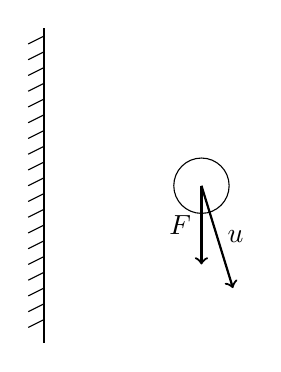
\begin{tikzpicture}
		\draw (-2,2) -- (-2,-2);
		\draw (-2.2, 1.8) -- (-2, 1.9);
		\draw (-2.2, 1.6) -- (-2, 1.7);
		\draw (-2.2, 1.4) -- (-2, 1.5);
		\draw (-2.2, 1.2) -- (-2, 1.3);
		\draw (-2.2, 1) -- (-2, 1.1);
		\draw (-2.2, 0.8) -- (-2, 0.9);
		\draw (-2.2, 0.6) -- (-2, 0.7);
		\draw (-2.2, 0.4) -- (-2, 0.5);
		\draw (-2.2, 0.2) -- (-2, 0.3);
		\draw (-2.2, 0) -- (-2, 0.1);
		\draw (-2.2,-1.8) -- (-2,- 1.7);
		\draw (-2.2,-1.6) -- (-2,- 1.5);
		\draw (-2.2,-1.4) -- (-2,- 1.3);
		\draw (-2.2,-1.2) -- (-2,- 1.1);
		\draw (-2.2,-1.0) -- (-2,- 0.9);
		\draw (-2.2,-0.8) -- (-2,- 0.7);
		\draw (-2.2,-0.6) -- (-2,- 0.5);
		\draw (-2.2,-0.4) -- (-2,- 0.3);
		\draw (-2.2,-0.2) -- (-2,- 0.1);
		\draw (0,0) circle (10pt);
		\draw [->,thick] (0,0) -- (0.4,-1.3) node[right, midway] {$\symbf{u}$};
		\draw [->, thick] (0,0) -- (0,-1) node[left, midway] {$\symbf{F}$};
	\end{tikzpicture}

	Applying reversibility, change $\symbf{F} \to -\symbf{F}$ so $\symbf{u} \to
	-\symbf{u}$:\\
	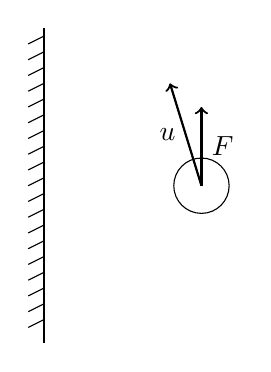
\begin{tikzpicture}
		\draw (-2,2) -- (-2,-2);
		\draw (-2.2, 1.8) -- (-2, 1.9);
		\draw (-2.2, 1.6) -- (-2, 1.7);
		\draw (-2.2, 1.4) -- (-2, 1.5);
		\draw (-2.2, 1.2) -- (-2, 1.3);
		\draw (-2.2, 1) -- (-2, 1.1);
		\draw (-2.2, 0.8) -- (-2, 0.9);
		\draw (-2.2, 0.6) -- (-2, 0.7);
		\draw (-2.2, 0.4) -- (-2, 0.5);
		\draw (-2.2, 0.2) -- (-2, 0.3);
		\draw (-2.2, 0) -- (-2, 0.1);
		\draw (-2.2,-1.8) -- (-2,- 1.7);
		\draw (-2.2,-1.6) -- (-2,- 1.5);
		\draw (-2.2,-1.4) -- (-2,- 1.3);
		\draw (-2.2,-1.2) -- (-2,- 1.1);
		\draw (-2.2,-1.0) -- (-2,- 0.9);
		\draw (-2.2,-0.8) -- (-2,- 0.7);
		\draw (-2.2,-0.6) -- (-2,- 0.5);
		\draw (-2.2,-0.4) -- (-2,- 0.3);
		\draw (-2.2,-0.2) -- (-2,- 0.1);
		\draw (0,0) circle (10pt);
		\draw [->,thick] (0,0) -- (-0.4,1.3) node[left, midway] {$\symbf{u}$};
		\draw [->, thick] (0,0) -- (0,1) node[right, midway] {$\symbf{F}$};
	\end{tikzpicture}\\
	Now apply symmetry: reflect the geometry top to bottom.\\
	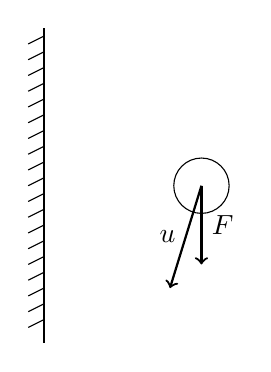
\begin{tikzpicture}
		\draw (-2,2) -- (-2,-2);
		\draw (-2.2, 1.8) -- (-2, 1.9);
		\draw (-2.2, 1.6) -- (-2, 1.7);
		\draw (-2.2, 1.4) -- (-2, 1.5);
		\draw (-2.2, 1.2) -- (-2, 1.3);
		\draw (-2.2, 1) -- (-2, 1.1);
		\draw (-2.2, 0.8) -- (-2, 0.9);
		\draw (-2.2, 0.6) -- (-2, 0.7);
		\draw (-2.2, 0.4) -- (-2, 0.5);
		\draw (-2.2, 0.2) -- (-2, 0.3);
		\draw (-2.2, 0) -- (-2, 0.1);
		\draw (-2.2,-1.8) -- (-2,- 1.7);
		\draw (-2.2,-1.6) -- (-2,- 1.5);
		\draw (-2.2,-1.4) -- (-2,- 1.3);
		\draw (-2.2,-1.2) -- (-2,- 1.1);
		\draw (-2.2,-1.0) -- (-2,- 0.9);
		\draw (-2.2,-0.8) -- (-2,- 0.7);
		\draw (-2.2,-0.6) -- (-2,- 0.5);
		\draw (-2.2,-0.4) -- (-2,- 0.3);
		\draw (-2.2,-0.2) -- (-2,- 0.1);
		\draw (0,0) circle (10pt);
		\draw [->,thick] (0,0) -- (-0.4,-1.3) node[left, midway] {$\symbf{u}$};
		\draw [->, thick] (0,0) -- (0,-1) node[right, midway] {$\symbf{F}$};
	\end{tikzpicture}

	Comparing with the original situation, we see there can be no lateral
	component of $\symbf{u}$.
\end{eg}

\subsubsection{Forces balance}
Since there is no inertia, the forces must balance. From the equations,
\begin{equation}
	\nabla \cdot \sigma = - \symbf{F} \implies \int_{\partial V} \sigma \cdot
	\symbf{n} \,\diffd S + \int_V \symbf{F} \,\diffd V = \symbf{0}
\end{equation}

This is a consistency check on stress boundary conditions. 

Similarly, in the absence of fluid sources,
\begin{equation}
	\nabla \cdot \symbf{u} = 0 \implies \int_{\partial V} \symbf{u} \cdot \symbf{n} \,
	\diffd S = 0
\end{equation}

This is a consistency check on velocity boundary conditions.

Likewise, torques balance, giving another consistency check on stress boundary
conditions.

\subsubsection{Work balances dissipation}
Intuitively, the flow has no kinetic energy (no inertia)  so any work done on
the fluid must be viscously dissipated instantaneously. We have
\begin{equation}
	\begin{aligned}
		\mathcal{D} &= 2\mu \int_V e_{ij} e_{ij} \, \diffd V \\
				&= \int (\sigma_{ij} + p \delta_{ij}) e_{ij} \, \diffd V \\
	&= \int \sigma_{ij} \frac{\partial u_i}{\partial x_j} + p e_{ii} \, \diffd V \\
	&= \int \frac{\partial}{\partial x_j} \sigma_{ij} u_i - u_i \frac{\partial
	\sigma_{ij}}{\partial x_j} \, \diffd V \\
	&= \int_{\partial V} \symbf{u} \cdot \symbfsf{\sigma} \cdot \symbf{n} \, \diffd S + \int
	\symbf{u} \cdot \symbf{F} \, \diffd V
	\end{aligned}
\end{equation}

The first term is the work done by surface forces at the boundary, and the
second term is the work done by body forces.

\subsubsection{Three Theorems Based on Dissipation Integrals}
\begin{lemma}
	\label{l1}
	If $\symbf{u}^I$ is an incompressible flow and $\symbf{u}^S$ is a Stokes flow
	with body force $\symbf{F}^S$ then 
	\begin{equation}
		2\mu \int e^{I} : e^{S} \, \diffd V = \int_{\partial V} \symbf{u}^I \cdot
		\sigma^S \cdot \symbf{n} \, \diffd S + \int_V \symbf{u}^I \cdot \symbf{F}^S \,
		\diffd V
	\end{equation}
\end{lemma}
Proof. Same as `work balances dissipation'.

\begin{theorem}
	Uniqueness theorem. Suppose $\symbf{u}_1, \symbf{u}_2$ are Stokes flows with the
	same boundary conditions and body forces, i.e. $\symbf{F}_1 = \symbf{F}_2$ in
	$V$ and either $\symbf{u}_1 = \symbf{u}_2$ or $\sigma_1 \cdot \symbf{n} = \sigma_2
	\cdot \symbf{n}$ on $\partial V$. Then $\symbf{u}_1 = \symbf{u}_2$.
\end{theorem}

Proof. Let $\symbf{u}^* = \symbf{u}_1 - \symbf{u}_2$. From lemma~\ref{l1}, 
\begin{equation}
	2\mu \int_V e^* : e^* \, \diffd V = 0
\end{equation}

Thus $e^* = 0$ in $V$. Hence we can deduce $\symbf{u}^*$ consists entirely of
rigid body motion: $\symbf{u}^* = \symbf{U} + \symbf{\Omega} \times \symbf{u}$. Using the
boundary conditions, we have $\symbf{U} = \symbf{\Omega} = 0$ thus $\symbf{u}_1 =
\symbf{u}_2$, i.e. Stokes flows are unique.

\lecture{14/10/20}
\begin{theorem}
	Reciprocal theorem. If $\symbf{u}_1$ and $\symbf{u}_2$ are Stokes flows in $V$
	then
	\begin{equation}
		\int_{\partial V} \symbf{u}_1 \cdot \sigma_2 \cdot \symbf{n} \, \diffd S +
		\int_V \symbf{u}_1 \cdot \symbf{F}_2 \, \diffd V = 
		\int_{\partial V} \symbf{u}_2 \cdot \sigma_1 \cdot \symbf{n} \, \diffd S +
		\int_V \symbf{u}_2 \cdot \symbf{F}_1 \, \diffd V
	\end{equation}

	That is, work done by forces of flow 1 against flow 2 = work done by
	forces of flow 2 against flow 1.
\end{theorem}

Proof. Apply the lemma twice.

\begin{theorem}
	Minimum Dissipation theorem. Among all the incompressible flows in $V$
	that satisfy given velocity boundary conditions, the dissipation is
	minimised by the Stokes flow $\symbf{u}^S$ with $\symbf{F}^s = \symbf{0}$
	satisfying the same velocity boundary conditions.
\end{theorem}

Proof. We have
\begin{equation}
	\begin{aligned}
		0 &\le 2\mu \int (e - e^S):(e-e^S) \, \diffd V \\
		  &\le 2\mu \int e:e - e^S:e^S \, \diffd V + 4\mu \int e^S : (e^S
		-e)\,\diffd V
	\end{aligned}
\end{equation}

Applying the lemma with $\symbf{u}^I = \symbf{u}^S - \symbf{u}$, the last term is $0$
since $\symbf{u}^I = 0$ on $\partial V$ and $\symbf{F}^S = 0$ on $V$. Thus
\begin{equation}
	0 \le \mathcal{D} - \mathcal{D}^S
\end{equation}

\begin{eg}
	\begin{enumerate}
		\hspace{2in}
		\item Consider an irregularly shaped body in a Stokes flow with
			inscribing circle $S_1$ with radius $a_1$ and circumscribing
			circle $S_2$ with radius $a_2$. Suppose the body experiences a
			force $\symbf{F}$ and has uniform velocity $\symbf{U}$.
		\begin{center}
			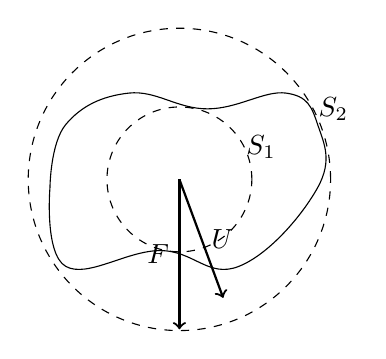
\begin{tikzpicture}[scale=0.4]
				\draw plot[smooth, tension=.7] coordinates {(-3.5, 0.5) (-3,
				2.5) (-1,3.5) (1.5,3) (4,3.5) (5,2.5) (5,0.5) (2.5,-2)
				(0,-1.5) (-3,-2) (-3.5,0.5)};
				\draw[dashed] (0.61,0.76) circle (2.3);
				\draw (5.5, 3) node {$S_2$};
				\draw[dashed] (0.61,0.76) circle (4.8);
				\draw (3.2, 1.8) node {$S_1$};
				\draw[thick, ->] (0.61,0.76) -- (0.61, -4) node [left, midway]
				{$\symbf{F}$};
				\draw[thick, ->] (0.61,0.76) -- (2, -3) node [right, midway]
				{$\symbf{U}$};
			\end{tikzpicture}
		\end{center}
		Applying the theorem by taking $\symbf{U}^S$ to be the Stokes flow past
		$S_1$ and $\symbf{U}^I$ to be the Stokes flow past $S_2$ superposed with
		solid body motion in the gap between $S_1$ and $S_2$, we have
		\begin{equation}
			(6\pi \mu a_1 U)U \le \symbf{F} \cdot \symbf{U} \le (6\pi \mu a_2 U)U
		\end{equation}

	\item Adding \emph{rigid} particles to a Stokes flow with given
		\emph{external} velocity boundary conditions increases dissipation
		and, if the particles are \emph{force-free} and \emph{torque-free},
		the apparent viscosity also increases.

		\begin{center}
			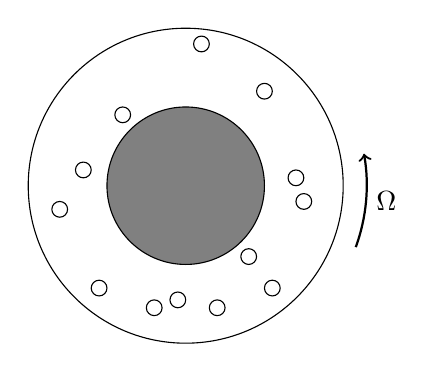
\begin{tikzpicture}
				\draw[fill=gray] (0,0) circle (1);
				\draw (0,0) circle (2);
				\draw (1.0, 1.2) circle (0.1);
				\draw (1.5, -0.2) circle (0.1);
				\draw (0.2, 1.8) circle (0.1);
				\draw (1.4, 0.1) circle (0.1);
				\draw (0.8, -0.9) circle (0.1);
				\draw (1.1, -1.3) circle (0.1);
				\draw (0.4, -1.55) circle (0.1);
				\draw (-0.1, -1.45) circle (0.1);
				\draw (-0.8, 0.9) circle (0.1);
				\draw (-1.1, -1.3) circle (0.1);
				\draw (-0.4, -1.55) circle (0.1);
				\draw (-1.3, 0.2) circle (0.1);
				\draw (-1.6, -0.3) circle (0.1);
				\draw[thick, ->] (2.16,-0.78) arc (-20:10:2.3)
				node[right,midway] {$\Omega$};
			\end{tikzpicture}
		\end{center}
	\item Inertia increases drag: consider $\rho \frac{\diffD \symbf{u}}{\diffD
		t}$ as $\symbf{F}$.
\end{enumerate}
\end{eg}

\subsection{Representation by Potentials}
Assume $\symbf{F}$ = 0, or that $\symbf{F}$ is conservative and absorbed by the
modified pressure. Consider the Stokes equations
\begin{align}
	\mu \nabla^2 \symbf{u} &= \nabla p \label{stokes1} \\
	\nabla \cdot \symbf{u} &= 0 \label{stokes2}
\end{align}

From these equations we have
\begin{equation}
	\begin{aligned}
		\nabla \cdot \eqref{stokes1} \& \eqref{stokes2} &\implies \nabla^2 p = 0 \implies
		p \hspace{.6em} \text{is harmonic} \\
		\nabla \times \eqref{stokes1} &\implies \nabla^2 \symbf{\omega} = 0
		\implies \text{vorticity}\hspace{.6em}\symbf{\omega} = \nabla \times
		\symbf{u} \hspace{.6em} \text{is harmonic} \\
		\nabla^2  \eqref{stokes1} &\implies \nabla^4 \symbf{u} = \symbf{0} \implies
		\symbf{u} \hspace{.6em} \text{is \emph{bi-harmonic}}
	\end{aligned}
\end{equation}

In two dimensions, we can use a stream-function so that $\symbf{u} = \nabla
\times (0,0,\psi)$. Then
\begin{equation}
	\omega_z = -\nabla^2 \psi \implies \nabla^4 \psi = 0
\end{equation}

Similarly, in axisymmetric spherical polars, $\symbf{u} = \nabla \times
(0,0,\frac{\Psi}{r \sin \theta})$. Then $\omega_\phi = -\frac{E^2 \Psi}{r\sin
\theta}$ and $E^4 \Psi = 0$ where
\begin{equation}
	E^2 = \frac{\partial^2}{\partial r^2} + \frac{\sin \theta}{r^2}
	\frac{\partial}{\partial \theta} \left( \sin \theta
	\frac{\partial}{\partial \theta}\right)
\end{equation}

Many exact solutions can be found in coordinate systems where the operators
$\nabla^2, \nabla^4, E^2$, etc are separable.

\subsubsection{Complex Variable Theory in 2D Flow}
Writing $z = x+iy, \bar{z} = x-iy$ gives
\begin{equation}
	\nabla^2 = 4 \frac{\partial^2}{\partial z \partial \bar{z}}
\end{equation}
Thus $f(x,y)$ analytic implies $f = f(z)$ or equivalently $\frac{\partial
f}{\partial \bar{z}} = 0$. Thus $\Re f$ and $\Im f$ are harmonic.

Similarly $\nabla^4 \psi = 0$ implies $\psi$ can be written as $\psi =
\Im(\bar{z}\phi + \chi)$ where $\phi(z), \chi(z)$ are analytic.

We can find clever exact solutions to difficult problems using this theory,
but it is limited to 2D.

\subsubsection{Papkovich-Neuber Solution}
Let $p = \nabla^2 \pi$ where
\begin{equation}
	\pi(\symbf{x}) = -\frac{1}{4\pi} \int \frac{p(\symbf{x'})}{\left|
	\symbf{x}-\symbf{x'}\right|} \, \diffd V
\end{equation}

Then the Stokes equations can be written $\nabla^2 \left( \mu \symbf{u} - \nabla
\pi\right) = 0$. Thus
\begin{equation}
	\mu \symbf{u} = \nabla \pi - \symbf{\Phi}
\end{equation}
where $\nabla^2 \symbf{\Phi} = 0$. Now $\nabla \cdot \symbf{u} = 0$ implies
$\nabla^2 \pi = \nabla \cdot \symbf{\Phi}$. Then
\begin{equation}
	\pi = \frac{1}{2}\left(\symbf{x}\cdot\symbf{\Phi} + \chi\right)
\end{equation}
where $\nabla^2 \chi = 0$. Thus \emph{any} Stokes flow with $\symbf{F} = 0$ can
be written in terms of a harmonic vector $\symbf{\Phi}$ and a harmonic scalar
$\chi$. The Stokes equations are then
\begin{equation}
	\begin{aligned}
		2\mu \symbf{u} &= \nabla \left(\symbf{x} \cdot \symbf{\Phi} + \chi\right) -
	2\symbf{\Phi} \\
	p &= \nabla \cdot \symbf{\Phi}
\end{aligned}
\end{equation}
which may also be re-written with the $2\mu$ factor absorbed by $p$.

Note the following.
\begin{enumerate}
	\item Any irrotational flow $2 \mu \symbf{u} = \nabla \chi$ is also a Stokes
		flow, though $p = 0$ and $\symbfsf{\sigma} = \nabla \nabla \chi$ which
		is different from an inviscid irrotational flow.
	\item It is sometimes possible to find a harmonic scalar $\phi$ with
		$\chi = \symbf{x} \cdot \nabla \phi - 2 \phi$. If so, $\chi$ can be
		eliminated by writing $\symbf{\Phi}' = \symbf{\Phi} + \nabla \phi$. For
		example, if $\chi$ has a spherical harmonic expansion we can eliminate
		all of the terms except the uniform strain $\chi/2\mu = \frac{1}{2}
		\symbf{x} \cdot \symsf{E} \cdot \symbf{x} \iff \symbf{u} = \symsf{E} \cdot
		\symbf{x}$, since $\chi = r^n Y_n^m(\theta,\phi) \iff \phi =
		\frac{r^n}{n-2} Y_n^m(\theta,\phi)$ which fails for $n=2$.
	\item Conversely, if $\symbf{\Phi} = \nabla \phi$ then we can get the same
		$\symbf{u}$ from $\chi = \symbf{x} \cdot \nabla \phi - 2\phi$, which is
		easier to calculate.
\end{enumerate}

\lecture{16/10/20}
\subsection{Solutions for points, spheres, and cylinders}
A point or sphere has no intrinsic direction or orientation, thus solutions on
these geometries should also have no intrinsic direction or orientation.

\subsubsection{Spherical harmonic functions}
Let $r = \abs{\x}$. Recall $\nabla^2 (\frac{1}{r}) = 0$ for $r \ne 0$. All
other spherical harmonic functions $\phi$ with $\phi \to 0$ as $r \to \infty$
are obtained from 
\begin{equation}
	\frac{1}{r}, \hspace{1em}\nabla \frac{1}{r},\hspace{1em} \nabla \nabla
	\frac{1}{r}, \hspace{1em}\text{etc.}
\end{equation}
The harmonic functions which are bounded as $r \to 0$ are
obtained from 
\begin{equation}
	r \cdot \inv{r} = 1,\hspace{1em} r^3 \nabla \inv{r} = -\x,\hspace{1em} r^5 \nabla
\nabla \inv{r},\hspace{1em} \dots,\hspace{1em} r^{2n+1} \nabla^n \inv{r}
\end{equation}

Compare with separable solutions, for example the $2n+1$ solutions in
spherical polars given by
\begin{equation}
\begin{pmatrix} r^n \\ r^{-n-1} \end{pmatrix} P_n^m(\theta) \begin{pmatrix}
\cos m \phi \\ \sin m\phi\end{pmatrix}
\end{equation}
where $P_n^m$ are \emph{associated Legendre functions} and $0 \le m \le n$.


Recall the following results.
\begin{equation}
	\begin{aligned}
		\nabla \x &= \symsf{I} \\
		\nabla r &= \frac{\x}{r} \\
		\nabla f(r) &= f'(r) \nabla r = f'(r) \frac{\x}{r}
	\end{aligned}
\end{equation}

Hence we have
\begin{equation}
	\begin{aligned}
		\nabla \inv{r} &= -\frac{\x}{r^3} \\
		\nabla \nabla \inv{r} &= -\frac{\symsf{I}}{r^3} +
		\frac{3\x\cdot\x}{r^5} \\
		\nabla_i \nabla_j \nabla_k \inv{r} &= \nabla_i \left(
		-\frac{\delta_{jk}}{r^3} + \frac{3x_j\cdot x_k}{r^5}\right)\\
		&= \frac{3(x_i \delta_{jk} + x_j \delta_{ik} + x_k \delta_{ij})}{r^5}
		- \frac{15 x_i x_j x_k}{r^7}
	\end{aligned}
\end{equation}

Note: these depend only on $\x$ and $r$ and thus have no preferred direction,
as hoped. We can use these functions to form Papkovich-Neuber potentials
$\symbf{\Phi}$ and $\chi$ by multiplying the harmonic functions above by constant
scalars, vectors or tensors and taking an appropriate number of dot products,
e.g. the following are all harmonic vectors
\begin{equation}
	\symbf{A} \inv{r}, \hspace{1em} \symsf{B} \cdot \nabla \inv{r},
	\hspace{1em} C \nabla \inv{r}, \hspace{1em} (\symbf{D} \cdot \nabla)\nabla
	\inv{r}, \hspace{1em} (\symsf{E}:\nabla\nabla)\nabla\inv{r}, \hspace{1em}
	\symbf{\Omega} \times \nabla \inv{r}
\end{equation}

It is useful to distinguish between \emph{true} and \emph{pseudo} tensors.
True / pseudo tensors keep / change sign upon reflection, e.g.
\begin{equation}
	T_{ijk}' = \pm R_{il} R_{jm} R_{kn} T_{lmn}
\end{equation}

Examples of true vectors are velocity $\symbf{u}$; force $\symbf{F}$; position $\x$;
 del $\nabla$; identity $\symsf{I}$.
Examples of pseudo vectors are angular velocity $\symbf{\Omega}$; torque
$\symbf{G}$; $\symbf{u} \times \x$; vorticity $\symbf{\omega} = \nabla \times \symbf{u}$.
Products obey the obvious parity rules, e.g. helicity $\symbf{u} \cdot
\symbf{\Omega}$ is a pseudo scalar.

\subsubsection{Solution due to a point force}
The Papkovich-Neuber solution due to a point force is a Green's function for
the Stokes equations. This problem is also known as a `Stokeslet'. Consider
the problem
\begin{equation}
	\begin{aligned}
		\nabla \cdot \symbfsf{\sigma} &= \mu \nabla^2 \symbf{u} - \nabla p = -
		\symbf{F} \delta(\x) \\
		\nabla \cdot \symbf{u} &= 0
	\end{aligned}
\end{equation}
with $\symbf{u} \to 0$ at infinity. The answer must be linear in $\symbf{F}$, but
otherwise has no orientation. The only choice is $\symbf{\Phi} = \alpha
\frac{\symbf{F}}{r}$. We could have tried $\symbf{F} \times \nabla \inv{r}$, but
this is a pseudo vector whilst $\symbf{\Phi}$ and $\chi$ need to be true since
$\symbf{u}$ is true. Similar arguments rule out other harmonic functions.

\lecture{19/10/20}
We have
\begin{equation}
	\begin{aligned}
		2\mu \symbf{u} &= \alpha \left( \nabla \left( \frac{\symbf{F} \cdot
			\x}{r}\right) - 2
		\frac{\symbf{F}}{r}\right) \\
		&= \alpha \left( \frac{\symbf{F} \cdot \symsf{I}}{r} -
	\frac{(\symbf{F}\cdot\x)\x}{r^3} - 2\frac{\symbf{F}}{r}\right) \\
	&= -\alpha \left( \frac{\symbf{F}}{r} + \frac{(\symbf{F}\cdot\x)\x}{r^3}\right)
\end{aligned}
\end{equation}

Thus the stress tensor is
\begin{equation}
	\symbfsf{\sigma} = \mu \left( \nabla \symbf{u} + \nabla \symbf{u}^T\right) -
	\left(\nabla \cdot \symbf{\Phi}\right)\symsf{I} = 3\alpha (\symbf{F} \cdot
	\symbf{x}) \frac{\x \x}{r^5}
\end{equation}

On any sphere $r=R$, $\symbf{n} = \frac{\x}{R}$, and
\begin{equation}
	\begin{aligned}
		2\mu \symbf{u}\cdot\symbf{n} &= -\frac{2\alpha}{R} \symbf{F}\cdot\symbf{n} \\
		\symbfsf{\sigma} \cdot \symbf{n} &= 3 \alpha \frac{(\symbf{F} \cdot
		\symbf{n}) \symbf{n}}{R^2}
	\end{aligned}
\end{equation}

To determine the constant $\alpha$ we can consider the surface volume flux and
the surface stress. The surface volume flux is
\begin{equation}
	\int_{r=R} \symbf{u}\cdot\symbf{n}\,\diffd S = -\frac{\alpha \symbf{F}}{\mu R}
	\cdot \int_{r=R} \symbf{n} \, \diffd S = 0
\end{equation}
which does not provide any information on $\alpha$. The surface forces should
equal $-\symbf{F}$. We have
\begin{equation}
	-\symbf{F} = \int_{r=R} \symbfsf{\sigma} \cdot \symbf{n} \, \diffd S = 3\alpha
	\symbf{F} \cdot \int_{r=R} \symbf{n} \symbf{n} \, \frac{\diffd S}{R^2} = 3 \alpha
	\symbf{F} \cdot \frac{4\pi}{3} \symsf{I} = 4\pi \alpha \symbf{F}
\end{equation}

Hence we choose $\alpha = -1/4\pi$. Thus the final solution is
\begin{equation}
	\symbf{u} = \symbf{F} \cdot \symsf{J}(\x), \hspace{2em} \symbfsf{\sigma} =
	\symbf{F} \cdot \symsf{K}(\x), \hspace{2em} p =
	\frac{\symbf{F}\cdot\x}{4\pi r^3}
\end{equation}
where $\symsf{J}$ is the \emph{Oseen tensor}:
\begin{equation}
	\symsf{J} = \frac{1}{8\pi \mu} \left( \frac{\symsf{I}}{r} +
		\frac{\x\x}{r^3}\right), \hspace{2em} \symsf{K} =
		-\frac{3}{4\pi} \frac{\x\x\x}{r^5}
\end{equation}

Finally, from incompressibility $\nabla \cdot \symbf{u} = 0$ and the Stokes
equations $\nabla \cdot \symbfsf{\sigma} = -\symbf{F}\delta(\x)$, we deduce
\begin{equation}
	\nabla \cdot \symsf{J} = 0, \hspace{2em} \nabla \cdot
	\symsf{K} = - \symsf{I}\delta(\x)
\end{equation}

Note that the velocity scales as $u \propto \inv{r}$: see
figure~\ref{fig:stokeslet}. This is slowly decaying compared to many forces
e.g. gravity which scales as $\inv{r^2}$. Thus particle interactions in Stokes
flow can occur on much larger scales than (for example) charge interactions.

\begin{figure}
\begin{center}
	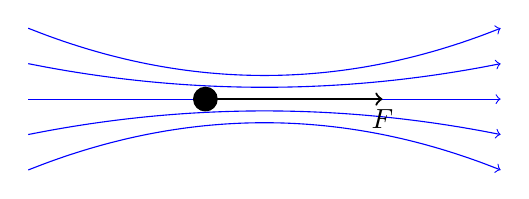
\begin{tikzpicture}[scale=1.5]
	\draw[smooth,domain=-2:2,blue,->] plot({\x},{0.05*\x*\x+0.1});
	\draw[smooth,domain=-2:2,blue,->] plot({\x},{0.1*\x*\x+0.2});
	\draw[smooth,domain=-2:2,blue,->] plot({\x},{-0.1*\x*\x-0.2});
	\draw[smooth,domain=-2:2,blue,->] plot({\x},{-0.05*\x*\x-0.1});
	\draw[smooth,domain=-2:2,blue,->] plot({\x},{0});
	\draw[fill=black] (-0.5,0) circle (0.1);
	\draw[thick,->] (-0.5, 0) -- (1, 0) node[below] {$\symbf{F}$};
\end{tikzpicture}
\end{center}
\caption{Stokeslet solution for a point force.}
\label{fig:stokeslet}
\end{figure}

\subsubsection{Source flow}
Consider a source of strength $Q$ with $\nabla \cdot \symbf{u} = Q \delta(\x)$.
This is referred to as a \emph{point volume source}. One can show the solution
is
\begin{equation}
	\symbf{u} = \frac{Q\x}{4\pi r^3}
\end{equation}
which is obtained using Papkovich-Neuber potentials
\begin{equation}
	\chi = \alpha \frac{Q}{r}, \hspace{2em} \symbf{\Phi} = \beta Q \nabla \inv{r}
\end{equation}

\subsubsection{Force dipole, stresslet, rotlet}
Further solutions for dipoles, quadrupoles, etc. can be found by taking
gradients of the Stokeslet and source solutions. For example, consider a
dipole.

\begin{center}
	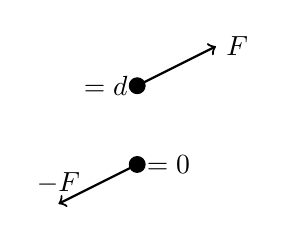
\begin{tikzpicture}
		\draw[fill] (0,0) circle (0.1) node[right] {$\x = \symbf{0}$};
		\draw[fill] (0,1) circle (0.1) node[left] {$\x = \symbf{d}$};
		\draw[thick, ->] (0,0) -- (-1,-0.5) node[above] {$-\symbf{F}$};
		\draw[thick, ->] (0,1) -- (1, 1.5) node[right] {$\symbf{F}$};
	\end{tikzpicture}
\end{center}

The Stokeslet solution is
\begin{equation}
	\symbf{u} = \symbf{F}\cdot\symsf{J} (\x-\symbf{d}) - \symbf{F} \cdot \symsf{J}(\x) =
	\symbf{F} \cdot (-\symbf{d}\cdot\nabla)\symsf{J}(\x) + \text{h.o.t.}
\end{equation}

Take the limit $\symbf{d} \to \symbf{0}$ with $\symbf{F}\symbf{d}$ fixed and split $-F_i
d_j$ into
\begin{enumerate}
	\item An isotropic part $-\frac{1}{3} F_k d_k \delta_{ij}$
	\item A symmetric traceless part
		\begin{equation}
			s_{ij} = -\frac{1}{2} (F_i d_j + F_j d_i) + \frac{1}{3} F_k d_k
			\delta_{ij}
		\end{equation}
	\item An antisymmetric part $-\frac{1}{2}\varepsilon_{ijk} G_k$ where
		$\symbf{G} = \symbf{d} \times \symbf{F}$
\end{enumerate}

The flow contribution from each of these components may then be calculated.
\begin{enumerate}
	\item The isotropic component gives no flow since $\nabla \cdot \symsf{J}
		= 0$
	\item This component is a \emph{stresslet} representing the following
		components of motion
		\begin{center}
			\begin{tikzpicture}[scale=0.7]
				\draw[fill] (0,1) circle (0.1);
				\draw[fill] (0,-1) circle (0.1);
				\draw[thick,->] (0,2) -- (0,1.1) node[right] {$\symbf{F}$};
				\draw[thick,->] (0,-2) -- (0,-1.1) node[right] {$-\symbf{F}$};
				\draw[fill] (-7,0) circle (0.1);
				\draw[fill] (-5,0) circle (0.1);
				\draw[thick,->] (-7,0) -- (-8,0) node[left] {$-\symbf{F}$};
				\draw[thick,->] (-5,0) -- (-4,0) node[right] {$\symbf{F}$};
				\draw[fill] (7,0) circle (0.1);
				\draw[fill] (5,0) circle (0.1);
				\draw[fill] (6, 1) circle (0.1);
				\draw[fill] (6, -1) circle (0.1);
				\draw[thick,->] (7,0) -- (7.8, 0) node[right] {$\symbf{F}/2$};
				\draw[thick,->] (5,0) -- (4.2, 0);
				\draw[thick,->] (6, 1.9) -- (6,1.1);
				\draw[thick,->] (6,-1.9) -- (6,-1.1);
			\end{tikzpicture}
		\end{center}

	\item This component is a \emph{rotlet} due to a point torque $\symbf{G}$.
		\begin{center}
			\begin{tikzpicture}
				\draw[fill] (0,0.5) circle (0.1);
				\draw[fill] (0,-0.5) circle (0.1);
				\draw[thick,->] (0,0.5) -- (-1, 0.5);
				\draw[thick,->] (0,-0.5) -- (1, -0.5);
				\draw[fill] (4, 0) circle (0.1);
				\draw[fill] (5, 0) circle (0.1);
				\draw[thick,->] (4,0) -- (4,1);
				\draw[thick,->] (5,0) -- (5,-1);
			\end{tikzpicture}
		\end{center}
\end{enumerate}

Both the stresslet and rotlet decay as $\inv{r^2}$.

\subsubsection{Rigid sphere with velocity U}
Consider a rigid sphere of radius $a$ moving uniformly  with velocity
$\symbf{U}$ in a Stokes flow. We have $\nabla \cdot \symbf{u} = 0$ and $\mu \nabla^2
\symbf{u} = \nabla p$ in $r > a$. We require $\symbf{u} \to 0$ as $r \to \infty$ and
$\symbf{u} = \symbf{U}$ on the sphere's surface $r=a$. The sphere is isotropic, so
we need harmonic functions of $\x, \symbf{U}$ which are linear in $\symbf{U}$; decay
at $\infty$; and are true tensors. We choose
\begin{equation}
	\frac{1}{2\mu} \symbf{\Phi} = \alpha \symbf{U} \inv{r}, \hspace{2em}
	\frac{1}{2\mu} \chi = \beta \symbf{u} \cdot \nabla \inv{r}
\end{equation}

This gives a solution which is a superposition of a Stokeslet and a source
dipole
\begin{equation}
	\symbf{u} = -\alpha \left( \frac{\symbf{U}}{r} +
		\frac{(\symbf{U}\cdot\x)\x}{r^3}\right) + \beta \left(
	-\frac{\symbf{U}}{r^3} + 3 \frac{(\symbf{U}\cdot\x)\x}{r^5}\right)
\end{equation}

Enforcing the boundary condition $\symbf{u} = \symbf{U}$ on $r=a$ requires
\begin{equation}
	\begin{aligned}
		-\frac{\alpha}{a} - \frac{\beta}{a^3} &= 1, \hspace{2em}
		-\frac{\alpha}{a} + 3 \frac{\beta}{a^3} = 0 \\
		\implies \alpha &= -\frac{3a}{4}, \hspace{1em} \beta = -\frac{a^3}{4}
	\end{aligned}
\end{equation}

Thus the final solution for a sphere in a Stokes flow is
\begin{equation}
	\symbf{u} = \frac{3}{4}\symbf{U}\left(\frac{a}{r} + \frac{a^3}{3r^3} \right) +
	\frac{3}{4} \frac{(\symbf{U}\cdot\x)\x}{r^2} \left( \frac{a}{r} -
	\frac{a^3}{r^3}\right)
\end{equation}

The corresponding pressure and vorticity, both of which are harmonic and due
to the Stokeslet, are
\begin{equation}
	p = \frac{3}{2}\mu a \frac{\symbf{U}\cdot\x}{r^3}, \hspace{2em}\symbf{\omega} =
	-\frac{1}{\mu} \nabla \times \symbf{\Phi} = \frac{3a}{2}\frac{\symbf{U} \times
	\symbf{x}}{r^3}
\end{equation}

\lecture{21/10/20}
\subsubsection{Force and stress on a translating sphere}
The flow at large distances is dominated by the $\inv{r}$ Stokeslet term with
strength $\symbf{F} = 6\pi \mu a \symbf{U}$. Since the force across $r = `\infty'$
must balance the force across $r=a$, we can see without further work that the
force by the fluid on the sphere i.e. drag $=-6\pi \mu a \symbf{U}$. In more
detail:
\begin{align}
	\symbfsf{\sigma} &= -p \symsf{I} + \mu \left( \nabla \symbf{u} + \nabla
	\symbf{u}^T\right) \\
	&= -\frac{3}{2} \mu a \frac{\symbf{U}\cdot\x}{r} + \frac{3}{4}\mu \left[
	\left(-\frac{a}{r^3} - \frac{a^3}{r^5}\right)\left(\x \symbf{U} + \symbf{U}
		\x\right)\right. \\
		&+ \left.\left(\symbf{U}\x + \x \symbf{U} + 2\symbf{U}\cdot\x
		\symsf{I}\right)\left(\frac{a}{r^3} - \frac{a^3}{r^5}\right) +
	\left(\symbf{U}\cdot\x\right)\left(-\frac{3a}{r^5}+\frac{5a^3}{r^7}\right)2\x\x\right]
	\\
	\implies\symbfsf{\sigma}\cdot\symbf{n}\mid_{r=a} &= -\frac{3}{2}\frac{\mu}{a}
	(\symbf{U}\cdot\symbf{n})\symbf{n} + \frac{3\mu}{4a}
	\left[-2(\symbf{n}(\symbf{U}\cdot\symbf{n}) + \symbf{U}) +
	(\symbf{U}\cdot\symbf{n})(-2)2\symbf{n}\right] \\
	&= -\frac{3\mu}{2a}\symbf{U}
\end{align}

Thus the drag on the sphere is
\begin{equation}
	\symbf{F} = \int_{r=a} \symbfsf{\sigma}\cdot \symbf{n}\,\diffd S =
	-\frac{3\mu}{2a} \symbf{U} \cdot 4\pi a^2 = -6\pi \mu a \symbf{U}
\end{equation}
as expected.

\subsubsection{Gravitational settling}
The force balance of weight, buoyancy, and drag gives the settling velocity of
a rigid sphere in a Stokes flow.
\begin{align}
	\frac{4}{3}\pi a^3 \rho_s \symbf{g} - \frac{4}{3}\pi a^3 \rho \symbf{g} - 6\pi
	\mu a \symbf{U} &= 0 \\
	\implies \symbf{U} &= \frac{2a^2}{9\mu}(\rho_s - \rho)\symbf{g} \propto a^2
\end{align}

\subsubsection{2D potentials}
The harmonic functions in two-dimensions which are bounded as $r \to \infty$
are
\begin{equation}
	\ln r, \hspace{1em} \nabla \ln r = \frac{\x}{r^2}, \hspace{1em} \nabla
	\nabla \ln r = \frac{\symsf{I}}{r^2} - \frac{2\x\x}{r^4}, \hspace{1em}\dots
\end{equation}
Similar to the 3D spherical case, the harmonic functions in two-dimensions
which are bounded as $r \to 0$ are
\begin{equation}
	1, \hspace{1em} r^2\nabla \ln r = \x, \hspace{1em}, \dots, \hspace{1em}
	r^{2n} \nabla^n \ln r
\end{equation}

The 2D Stokeslet solution follows from the Papkovich-Neuber potentials
$\symbf{\Phi} = \frac{\symbf{F}}{2\pi} \ln r$ which gives
\begin{align}
	\symbf{u} &= \symbf{F}\cdot\symsf{J}^{2D} \\
	p &= \frac{\symbf{F}\cdot\x}{2\pi r^2} \\
	\symbfsf{\sigma} &= \symbf{F} \cdot \symsf{K}^{2D} \\
	\symsf{J}^{2D} &= \frac{1}{4\pi \mu} \left( -\ln r \symsf{I} +
	\frac{\x\x}{r^2}\right) \\
	\symsf{K}^{2D} &= -\frac{1}{\pi} \frac{\x\x\x}{r^4}
\end{align}

The 2D Stokeslet solution corresponds to a line force $\symbf{F}$ \emph{per unit
length}. Note that $\symbf{u} \not\to 0$ as $r \to \infty$ for a line force,
though $\symbf{u} \to 0$ for line dipoles, line quadrupoles, etc.

\subsection{Motion of rigid particles}
\subsubsection{The resistance matrix}
A rigid particle moving with velocity $\symbf{U} + \symbf{\Omega} \times \x$ through
fluid otherwise at rest exerts a force $\symbf{F}$ and a couple $\symbf{G}$ on the
fluid. By linearity,
\begin{equation}
\begin{pmatrix} \symbf{F} \\ \symbf{G}\end{pmatrix} = \begin{pmatrix} \symsf{A} & 
\symsf{B} \\ \symsf{C} & \symsf{D} \end{pmatrix} \begin{pmatrix} \symbf{U} \\
\symbf{\Omega} \end{pmatrix}
\end{equation}
where the tensors $\symsf{A} - \symsf{D}$ depend on the size, shape, and
orientation of the body. We refer to this matrix as the \emph{resistance
matrix}. We have 

\begin{equation}
	\int_{\text{body}} \symbf{u}\cdot\symbfsf{\sigma}\cdot\symbf{n}\,\diffd S = \int
	(\symbf{U} + \symbf{\Omega}\times\x)\cdot\symbfsf{\sigma}\cdot\symbf{n}\,\diffd S
	= \symbf{U} \cdot \symbf{F} + \symbf{\Omega} \cdot \symbf{G}
\end{equation}

Similarly, from the reciprocal theorem (with $\symbf{F} = 0$), for all $\symbf{U}_1,
\symbf{\Omega}_1, \symbf{U}_2, \symbf{\Omega}_2$, 
\begin{equation}
	(\symbf{U}_1, \symbf{\Omega}_1)\begin{pmatrix} \symsf{A} & \symsf{B} \\
	\symsf{C} & \symsf{D} \end{pmatrix} \begin{pmatrix} \symbf{U}_2 \\
	\symbf{\Omega}_2\end{pmatrix} = 
	(\symbf{U}_2, \symbf{\Omega}_2)\begin{pmatrix} \symsf{A} & \symsf{B} \\
	\symsf{C} & \symsf{D} \end{pmatrix} \begin{pmatrix} \symbf{U}_1 \\
	\symbf{\Omega}_1\end{pmatrix} = 
	(\symbf{U}_1, \symbf{\Omega}_1)\begin{pmatrix} \symsf{A}^T & \symsf{C}^T \\
	\symsf{B}^T & \symsf{D}^T \end{pmatrix} \begin{pmatrix} \symbf{U}_2 \\
	\symbf{\Omega}_2\end{pmatrix}
\end{equation}

Hence $\symsf{A} = \symsf{A}^T$, $\symsf{D} = \symsf{D}^T$ so $\symsf{A}$
and $\symsf{D}$ are diagonalisable, and $\symsf{B} = \symsf{C}^T$, i.e. the
force from pure rotation is equal to the couple from pure translation. Since
the viscous dissipation is positive, the resistance matrix is positive
definite, so invertible.

\lecture{23/10/20}
\begin{eg}
	\hspace{2in}
	\begin{enumerate}
		\item A body with $3$ independent planes of reflectional symmetry has
			$\symsf{B} = \symsf{C} = 0$.
		\item A cube falls with the same speed (and no rotation) in all
			orientations since $\symsf{A} \propto \symsf{I}$.
		\item $\symsf{A}$ and $\symsf{D}$ are known for ellipsoids, and
			therefore for rods and discs which are limits of ellipsoids.
	\end{enumerate}
\end{eg}

The resistance matrix and its inverse the \emph{mobility matrix} are sometimes
extended to describe a rigid particle placed in a background linear flow
$\symbf{u}^\infty = \symbf{U}^\infty + \symbf{\Omega}^\infty \times \x +
\symsf{E}^\infty \cdot \x$, as 
\begin{equation}
\begin{pmatrix} \symbf{F} \\ \symbf{G} \\ \symsf{S} \end{pmatrix} = \begin{pmatrix}
&&\\&12 \times 12 & \\ &&\end{pmatrix} \begin{pmatrix} \symbf{U}-\symbf{U}^\infty \\
\symbf{\Omega} - \symbf{\Omega}^\infty \\ \symsf{E}^\infty \end{pmatrix}
\end{equation}

where $\symsf{S}$ is the stresslet exerted by the particle.


If $\symsf{E}^\infty = 0$, a force-free, couple-free particle just translates
and rotates with the flow. If $\symsf{E}^\infty \ne 0 $ then the particle
generates a stresslet. In general, the extra dissipation
\begin{equation}
	\symbf{F}\cdot(\symbf{U} - \symbf{U}^\infty) + \symbf{G} \cdot (\symbf{\Omega} -
	\symbf{\Omega}^\infty) + \symsf{S}:\symsf{E}^\infty
\end{equation}
is positive by the minimum dissipation theorem, thus the extended
matrix is positive definite, so invertible.

This is useful because it gives the leading order effects for a small particle
of size $a$ in a flow of larger lengthscale $L$:
\begin{equation}
	\symbf{u}^\infty(\x) = \symbf{u}^\infty(0) + \x \cdot \nabla \symbf{u}^\infty(0) +
	\mathcal{O}(a^2/L^2)
\end{equation}

\subsection{Fax\'{e}n relations}
Consider the behaviour of a rigid particle placed in an arbitrary unbounded
Stokes flow $\symbf{u}^\infty(\x)$. Can we find the particle motion $\symbf{u}^P =
\symbf{U} + \symbf{\Omega} \times \x$? Let $\symbf{u}'$ be the \emph{perturbation flow}
$\symbf{u}' = \symbf{u} - \symbf{u}^\infty$, which has boundary conditions
\begin{align}
	\symbf{u}' &\to 0 \hspace{1em} \text{as} \,\,\, \abs{\x} \to \infty \\
	\symbf{u}' &= \symbf{u}^P - \symbf{u}^\infty(\x) \hspace{1em} \text{on particle}
\end{align}
and $\hat{\symbf{u}}$ a `test' flow due to particle translation with arbitrary
velocity $\hat{\symbf{V}}$. By linearity, 
\begin{equation}
	\hat{\symbfsf{\sigma}} = \hat{\symbfsf{\Sigma}}(\x) \cdot
	\hat{\symbf{V}}
\end{equation}
for some third rank tensor $\hat{\symbfsf{\Sigma}}$. The reciprocal theorem for
$\symbf{u}'$ and $\hat{\symbf{u}}$ gives
\begin{equation}
	\hat{\symbf{V}} \cdot \int_{S_P} \symbfsf{\sigma}' \cdot \symbf{n}\,\diffd S =
	\hat{\symbf{V}} \cdot \int (\symbf{u}^P - \symbf{u}^\infty(\x))\cdot
	\hat{\symbfsf{\Sigma}} \cdot \symbf{n}\,\diffd S
\end{equation}
Now $\hat{\symbf{V}}$ is arbitrary and contribution from $\int \symbf{u}^P \cdot
\hat{\symbfsf{\Sigma}}\cdot\symbf{n}\,\diffd S$ is given by
\begin{equation}
\begin{pmatrix} \symbf{U} & \symbf{\Sigma}\end{pmatrix} \begin{pmatrix} \symsf{A} &
\symsf{B} \\ \symsf{B}^T & \symsf{D} \end{pmatrix} \begin{pmatrix}
\hat{\symbf{V}} \\ \symbf{0} \end{pmatrix}
\end{equation}

Hence we have \emph{Fax\'{e}n's first formula}
\begin{equation}
	\symbf{F} = \symsf{A}\cdot\symbf{U} + \symsf{B} \cdot \symbf{\Omega} - \int
	\symbf{u}^\infty(\x) \cdot
	\hat{\symbfsf{\Sigma}}\cdot\symbf{n}\,\diffd S
\end{equation}

Similar Fax\'{e}n relations can be obtained for the couple $\symbf{G}$ and
stresslet $\symsf{S}$ exerted, by using other test flows.

\begin{eg}
	For a sphere, we have $\hat{\symbfsf{\Sigma}}\cdot\symbf{n} =
	\frac{3\mu}{2a} \symsf{I}$ on $r=a$, where $\symbf{n}$ is \emph{into} the
	particle. We also have
	\begin{equation}
		\symsf{A} = 6\pi \mu a \symsf{I}, \hspace{2em} \symsf{B} = 0
	\end{equation}
	which gives a translation velocity
	\begin{equation}
		\symbf{U} = \frac{\symbf{F}}{6\pi\mu a} + \frac{1}{4\pi a^2} \int
		\symbf{u}^\infty(\x) \, \diffd S
	\end{equation}
	where the last term is an average of $\symbf{u}^\infty$ over the surface.
	Moreover, we can Taylor expand this far field velocity
	\begin{equation}
		\symbf{u}^\infty(\x) = \symbf{u}^\infty(\symbf{0}) + \x \cdot \nabla \symbf{u}^\infty(\symbf{0})
		+ \frac{1}{2}\x\x:\nabla\nabla \symbf{u}^\infty(\symbf{0}) + \dots
	\end{equation}
	Therefore we have
	\begin{equation}
		\frac{1}{4\pi a^2} \int_{r=a} \symbf{u}^\infty(\x) \, \diffd S =
		\symbf{u}^\infty(\symbf{0}) + 0 + \frac{1}{8\pi a^2} \int_{r=a} \x \x \, \diffd
		S : \nabla \nabla \symbf{u}^\infty(\symbf{0}) + \dots
	\end{equation}
	Odd terms, for example $\int_{r=a} \x\x\x\,\diffd S = 0$ by symmetry. Even
	terms are isotropic and give $\nabla^{2n} \symbf{u}^\infty(\symbf{0})$, but by
	Stokes equations $\nabla^4 \symbf{u}^\infty = \symbf{0}$. Hence
	\begin{equation}
		\symbf{U} = \frac{\symbf{F}}{6\pi\mu a} + \symbf{u}^\infty(\symbf{0}) + \frac{a^2}{6}
		\nabla^2 \symbf{u}^\infty(\symbf{0})
	\end{equation}
\end{eg}

\paragraph{Application to two sedimenting spheres.}
Consider two rigid spheres of radius $a$ sedimenting under a given force
$\symbf{F}$. We wish to calculate the flal speed $\symbf{U}$ to
$\mathcal{O}(a^3/R^3)$. One sphere moves in the far-field flow of the other
sphere, which itself depends on the force, couple, and stresslet exerted at
leading order. $\symbf{F}$ and $\symbf{G} = 0$ are the same for each sphere, hence
this far field is the same as for an isolated sphere up to
$\mathcal{O}(a^4/R^4)$. Fax\'{e}n gives an $\mathcal{O}(a^3/R^3)$ correction
to $\symbf{U}$ from the $\frac{a^2}{6}\nabla^2$ term.

\lecture{26/10/20}
\subsection{Integral representations of Stokes flow}
\label{ss:integralrep}
\subsubsection{Basic integral identity}
Consider a Stokes flow $\symbf{u}$ and a Stokeslet flow $\symbf{u}^S$ due to a point force
$\symbf{F}$ at $\y$. We have $\nabla \cdot \symbf{u} = \nabla \cdot \symbf{u}^S = 0$ and
\begin{equation}
	\nabla \cdot \symbfsf{\sigma} = -\symbf{f}, \hspace{2em} \nabla \cdot
	\symbfsf{\sigma}^S = -\symbf{F} \delta(\x-\y)
\end{equation}

Apply the reciprocal theorem with $\symbf{u}_1 = \symbf{u}, \symbf{u}_2 = \symbf{u}^S$. We have
\begin{equation}
	\int_V \symbf{u} \cdot \symbf{F} \delta(\x-\y) \, \diffd V + \int_{\partial V} \symbf{u}
	\cdot \left( \symbf{F} \cdot
		\symsf{K}(\x-\y)\right)\cdot\symbf{n}\,\diffd S = \int_v
		\left( \symbf{F} \cdot \symsf{J}(\x-\y)\right) \cdot \symbf{f} \, \diffd V
		+ \int_{\partial V} \left( \symbf{F} \cdot
		\symsf{J}(\x-\y)\right)\cdot\symbfsf{\sigma}\cdot\symbf{n}\,\diffd S
\end{equation}

Note by definition $J$ is even and $K$ is odd, so $\symsf{J}(\x-\y) =
\symsf{J}(\y-\x)$ and $\symsf{K}(\x-\y) =
-\symsf{K}(\y-\x)$. Also, $\symbf{F}$ is arbitrary so may be
factored out by the quotient theorem. We also have from the sampling property
of the delta function
\begin{equation}
	\int_V \phi(\x) \delta(\x-\y)\,\diffd V = \begin{cases} \phi(\y) & \y \in
		V \\ 0 & \y \not\in V \\ \frac{1}{2}\phi(\y) & \y \in \partial V
	\end{cases}
\end{equation}
Note we require $\y\in\partial V$ to be a smooth point of $\partial V$ for
this to hold. Hence
\begin{equation}
	\int_V \symsf{J}(\y-\x)\cdot\symbf{f}(\x)\,\diffd V + \int_{\partial V}
	\symsf{J}(\y-\x)\cdot\symbfsf{\sigma}\cdot\symbf{n}\,\diffd S +
	\int_{\partial V}
	\symbf{u}(\x)\cdot\symsf{K}(\y-\x)\cdot\symbf{n}\,\diffd S =
	\begin{cases}
		\symbf{u}(\y) & \y \in V \\ 0 & \y\not\in V \\ \frac{1}{2} \symbf{u}(\y) & \y
	\not\in \partial V \end{cases}
\end{equation}

\begin{enumerate}
	\item The above follows the sign conventions: $\symbf{n}$ is out of $v$, and
		we have $\y - \x$ as  the argument.
	\item $\symbf{f}$ is often not included, i.e. there is no body force or
		$\symbf{f}$ is absorbed into modified pressure
	\item The jump in the RHS comes from the $\symsf{K}$ integral
		which depends on $\inv{r}$ which jumps when $\y$ crosses $\partial
		V$.
	\item Usually we only know $\symbfsf{\sigma}\cdot\symbf{n}$ or $\symbf{u}$ on
		$\partial V$. In general, we solve as an integral equation for
		whichever is not specified with $\y \in \partial V$ and then
		substitute to find $\symbf{u}$ elsewhere.
\end{enumerate}

\subsubsection{Far-field approximations/multipole expansion for a moving body}
For a body of size $a$ and for $\abs{\y} \gg a$ we have by Taylor expanding
\begin{align}
	\symsf{J}(\y-\x) &\approx \symsf{J}(\y) - \x \cdot \nabla \symsf{J}(\y)
	+ \mathcal{O}(\frac{a^2}{y^3}) \\
	\symsf{K}(\y-\x) &\approx \symsf{K}(\y) +
	\mathcal{O}(\frac{a^2}{y^3})
\end{align}
Assuming $\symbf{f} = 0$, substitute this into the basic integral representation
to obtain after some messy algebra
\begin{equation}
	\symbf{u}(\y) \approx \symbf{F} \cdot \symsf{J}(\y) + \frac{\symbf{G} \times
		\y}{8\pi\mu \abs{\y}^3} + \frac{Q\y}{4\pi\abs{\y}^3} - \frac{3 (\y
		\cdot \symsf{S} \cdot \y)\y}{8\pi\mu \abs{\y}^5} +
		\mathcal{O}(\frac{a^2}{y^3})
\end{equation}
where the first term is $\mathcal{O}(\inv{y})$, the three following terms are
$\mathcal{O}(\frac{a}{y^2})$ and (using $\symbf{n}$ out of body)
\begin{align}
	\symbf{F} &= -\int \symbfsf{\sigma}\cdot\symbf{n}\,\diffd S = \text{force exerted
	by body}\\
	\symbf{G} &= -\int \x \times \symbfsf{\sigma} \cdot \symbf{n}\,\diffd S =
	\text{couple exerted by body} \\
	Q &= \int \symbf{u} \cdot \symbf{n} \,\diffd S = \text{source strength (vanishes for
	rigid body)} \\
	\symsf{S} &= \int \left[ \frac{1}{2} \left( \x
			(\symbfsf{\sigma}\cdot\symbf{n}) - 2 \mu \symbf{u} \symbf{n}\right) +
			\frac{1}{2}\left( \x
				(\symbfsf{\sigma}\cdot\symbf{n}) - 2 \mu \symbf{u} \symbf{n}\right)^T -
				\frac{1}{3}\symsf{I} \text{tr}\left( \x
			(\symbfsf{\sigma}\cdot\symbf{n}) - 2 \mu \symbf{u} \symbf{n}\right)\right] \,
			\diffd S = \text{stresslet exerted}
\end{align}

Note the terms involving $\symbf{u}$ in the integrand for $\symsf{S}$ vanish for a
rigid body.

\begin{enumerate}
	\item The far-field of a moving body is related to the force exerted by
		the body, not its velocity.
	\item The far-field of a force-free, couple-free, incompressible body is a
		stresslet.
\end{enumerate}

\lecture{28/10/20}
\subsubsection{Representation for droplets}
Consider a droplet occupying a volume $V_1$ with viscosity $\lambda \mu$ in a
surrounding fluid volume $V_2$ with viscosity $\mu$. Let $\symbf{n}$ be
\emph{out} of the droplet. Use viscosity $\mu$ in the Stokeslet tensor
$\symsf{J}$. We assume for simplicity that there is no body force, $\symbf{f} =
0$, and the far field is at rest, $\symbf{u} \to 0$ as $r \to \infty$. Applying
the basic integral identity to each of $V_1$ and $V_2$ we have
\begin{align}
	\int_{\partial V} \frac{1}{\lambda} \symsf{J} \cdot \symbfsf{\sigma_1}
	\cdot \symbf{n} + \symbf{u}_1 \cdot \symsf{K} \cdot \symbf{n} \, \diffd S
	&= \begin{cases} \symbf{u}_1 & \y \in V_1 \\ 0 & \y \in V_2 \\ \frac{1}{2}\symbf{u}_1 &
	\y \in \partial V \end{cases} \label{eq:drop1} \\
	-\int_{\partial V} \frac{1}{\lambda} \symsf{J} \cdot \symbfsf{\sigma_2}
	\cdot \symbf{n} + \symbf{u}_2 \cdot \symsf{K} \cdot \symbf{n} \, \diffd S
	&= \begin{cases} \symbf{u}_2 & 0 \in V_1 \\ \symbf{u}_2 & \y \in V_2 \\ \frac{1}{2}\symbf{u}_2 &
	\y \in \partial V \end{cases} \label{eq:drop2} \\
\end{align}
Note the $-$ sign in \eqref{eq:drop2} is because $\symbf{n}$ points into $V_2$.
Now $\symbf{u}_1 = \symbf{u}_2 = \symbf{u}$ (say) on $\partial V$. So $\lambda$\eqref{eq:drop2} +
\eqref{eq:drop1} implies
\begin{equation}
	\int_{\partial V} \symsf{J}(\y-\x) \cdot (\symbfsf{\sigma_1} \cdot \symbf{n}
	- \symbfsf{\sigma_2} \cdot \symbf{n})\,\diffd S_x + (\lambda-1) \int_{\partial
		V} \symbf{u} \cdot \symsf{K}(\y-\x)\cdot\symbf{n}\,\diffd S_x =
		\begin{cases} \lambda \symbf{u}_1 & \y \in V_1 \\ \symbf{u}_2 & \y \in V_2 \\
		\frac{1}{2}(\lambda+1)\symbf{u} & \y \in \partial V \end{cases}
\end{equation}

This integral equation is the basis for powerful numerical methods to
determine droplet shapes and evolution. 

\begin{eg}
	Relaxation of a drop under constant surface tension. The flow is driven by
	$\symbfsf{\sigma_2} \cdot \symbf{n} - \symbfsf{\sigma_1} \cdot \symbf{n} = \gamma
	(\nabla \cdot \symbf{n})\symbf{n}$. We consider $\y \in \partial V$ to find the
	interfacial motion:
	\begin{enumerate}
		\item $\lambda = 1$: we have 
			\begin{equation}
				\symbf{u}(\y) = -\gamma \int_{\partial V} (\nabla \cdot
				\symbf{n})\symbf{n}\cdot\symsf{J}(\y-\x)\,\diffd S_x
			\end{equation}
			hence the interfacial velocity is determined directly by the
			current shape of the droplet. It requires only an integral of the
			forcing over the boundary (a `membrane' of Stokeslets) to
			determine $\symbf{u}$.
		\item $\lambda \ne 1$: to solve the integral equation
			\begin{equation}
				\frac{\lambda + 1}{2} \symbf{u}(\y) = -\gamma \int_{\partial V}
				(\nabla \cdot \symbf{n})\symbf{n}\cdot\symsf{J}\,\diffd S_x +
				(\lambda -1) \int_{\partial V} \symbf{u}(\x) \cdot
				\symsf{K} \cdot \symbf{n} \, \diffd S_x
			\end{equation}
			for $\symbf{u}$, we discretize the integrals and invert the resulting
			matrix equation. The integral equation is singular (so the matrix
			equation is singular) if $\lambda = 0$ or $\lambda = \infty$. The
			null eigenmodes are the $6$ rigid body motions ($\lambda =
			\infty$) and bubble enlargement ($\lambda = 0$); the corresponding
			solubility conditions are the consistency conditions on boundary
			conditions.
	\end{enumerate}
\end{eg}
\subsubsection{Representation by Stokeslets alone}
Consider the flow outside a moving body, e.g. swimming micro-organisms. Though
we are interested in the flow $\symbf{u}$ in $V$, we imagine a flow $\symbf{u}^*$ in $V^*$
with $\mu^* = \mu$ and $\symbf{u}^* = \symbf{u}$ on $\partial V$. Such a flow exists if
$\int_{\partial V} \symbf{u} \cdot \symbf{n} \, \diffd S = 0$.
\begin{center}
	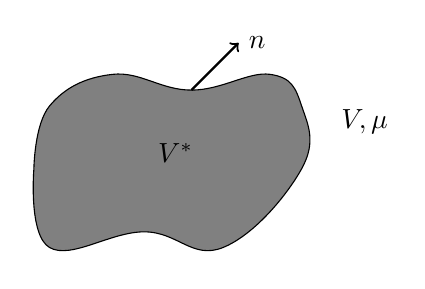
\begin{tikzpicture}[scale=0.4]
		\draw[fill=gray] plot[smooth, tension=.7] coordinates {(-3.5, 0.5) (-3,
		2.5) (-1,3.5) (1.5,3) (4,3.5) (5,2.5) (5,0.5) (2.5,-2)
		(0,-1.5) (-3,-2) (-3.5,0.5)};
		\draw[thick,->] (1.5,3) -- (3, 4.5) node[right] {$\symbf{n}$};
		\draw (1,1) node {$V^*$};
		\draw (7,2) node {$V, \mu$};
	\end{tikzpicture}
\end{center}

The previous result for drops gives
\begin{equation}
	\symbf{u}(\y) = \int_{\partial V} \symsf{J}(\y-\x) \cdot \symbf{f}_S(\x) \, \diffd
	S
\end{equation}
where $\symbf{f}_S = (\symbfsf{\sigma}^* - \symbfsf{\sigma})\cdot\symbf{n}$ is the
Stokeslet density. Note:
\begin{enumerate}
	\item $\symbfsf{\sigma}^*$ may not be the real stress in $V^*$ unless the
		body really is fluid with $\mu = \mu^*$.
	\item If the body is rigid then $\symbf{u}^*$ is rigid-body motion and
		$\symbfsf{\sigma}^* = \symbf{0}$. In this case $\symbf{f}_S$ is the stress
		$-\symbfsf{\sigma}\cdot\symbf{n}$ exerted by the body on the fluid. The
		external flow depends \emph{only} on $\symbfsf{\sigma}\cdot\symbf{n}$ and
		\emph{not} on $\symbf{u}$.
\end{enumerate}


\section{Approximations and applications}
\subsection{Slender-body theory}
\label{ss:slenderbody}
Consider the case of a solid, perhaps flexible, body e.g. flagellum, or fibre
in a flow. Our aim is to calculate resistance to prescribed motion
$\symbf{V}(s) = \dot{\symbf{X}}$ in background flow $\symbf{u}^\infty(\x)$. 

\begin{center}
	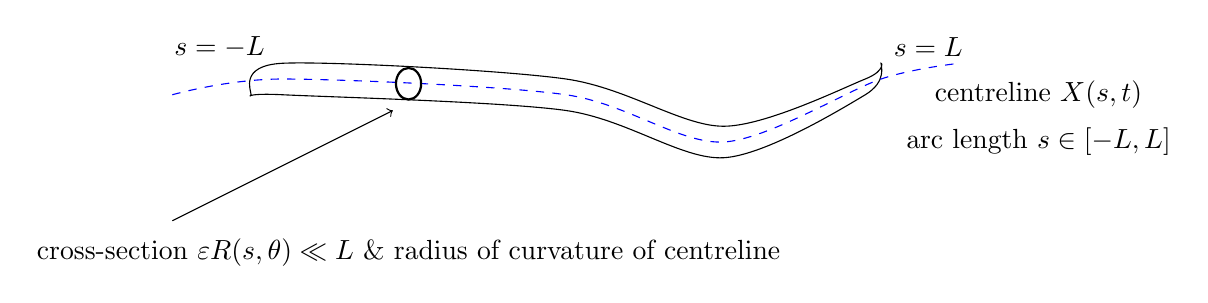
\begin{tikzpicture}[scale=2]
		\draw plot [smooth cycle] coordinates {(-2,0) (-1.8, 0.2) (0, 0.1) (1,
		-0.2) (1.9, 0.1) (2, 0.2) (1.9, 0) (1, -0.4) (0, -0.1) (-1.8, 0)};
		\draw[blue,dashed] plot [smooth] coordinates {(-2.5, 0) (-1.8, 0.1) (0,
		0) (1, -0.3) (2, 0.1) (2.5, 0.2)};
		\draw[thick] (-1, 0.07) ellipse (0.08 and 0.1);
		\draw (-1, -1) node {cross-section $\varepsilon R(s, \theta) \ll L$ \&
		radius of curvature of centreline};
		\draw[->] (-2.5, -0.8) -- (-1.1, -0.1);
		\draw (3, 0) node {centreline $\symbf{X}(s,t)$};
		\draw (3, -0.3) node {arc length $s \in \left[-L,L\right]$};
		\draw (2.3, 0.3) node {$s=L$};
		\draw (-2.2, 0.3) node {$s=-L$};
	\end{tikzpicture}
\end{center}

Since the body is slender, we can approximate the surface distribution of
Stokeslets by a distribution along the centreline, i.e.
\begin{equation}
	\symbf{u}(\y) = \symbf{u}^\infty(\y) + \int_{-L}^L \symsf{J}(\y - \symbf{X}(s)) \cdot
	\symbf{f}(s) \, \diffd s
\end{equation}

\lecture{30/10/20}
Note the integral is the first term in a far-field expansion for a ring of
Stokeslets. Consider a point $\y = \X(s_0) + \varepsilon \symbf{R}(s_0,\theta)$
on the surface of the body. 
\begin{center}
	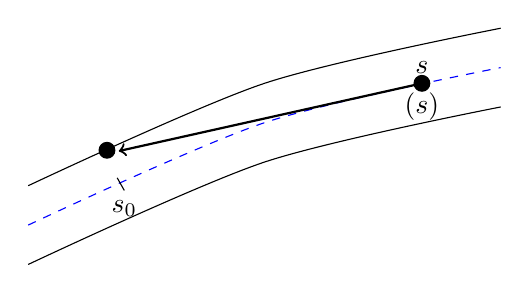
\begin{tikzpicture}
		\draw plot[smooth] coordinates {(-3,0) (0, 1.3) (3,2)};
		\draw plot[smooth] coordinates {(-3,-1) (0, 0.3) (3,1)};
		\draw[dashed,blue] plot[smooth] coordinates {(-3,-0.5) (0, 0.8) (3,1.5)};
		\draw[fill] (2, 1.3) circle (0.1);
		\draw[fill] (-2, 0.45) circle (0.1);
		\draw (-2,0.45) node[above] {$\y$};
		\draw (2, 1.3) node[below] {$\X(s)$};
		\draw (2, 1.3) node[above] {$s$};
		\draw (-1.87, 0.1) -- (-1.78, -0.06) node[below] {$s_0$};
		\draw[thick,->] (2, 1.3) -- (-1.85, 0.44);
	\end{tikzpicture}
\end{center}

The integrand is proportional to $\frac{1}{\abs{\y-\X(s)}}$ and behaves like
so:
\begin{center}
	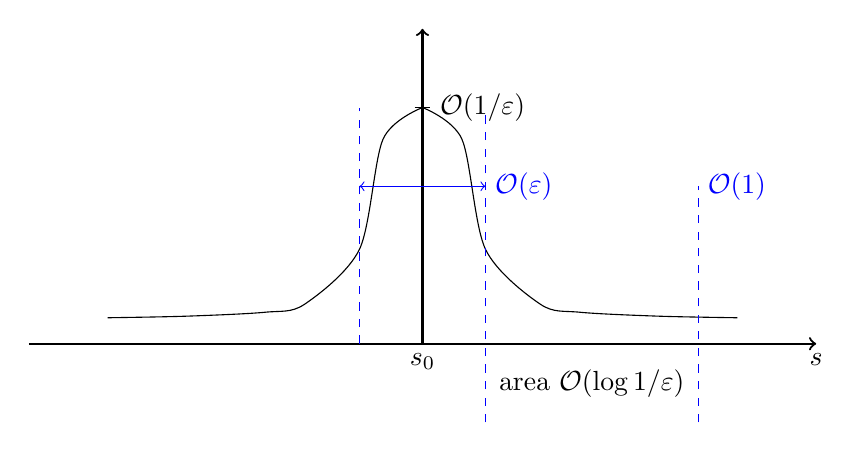
\begin{tikzpicture}
		\draw[thick,->] (-5, 0) -- (5,0) node[below] {$s$};
		\draw[thick,->] (0,0) -- (0, 4); 
		\draw (0,0) node[below] {$s_0$};
		\draw plot[smooth] coordinates { (0,3) (0.5,2.6) (0.8,1.2) (1.5,0.5)
		(2, 0.4) (3, 0.35) (4, 0.33)};
		\draw plot[smooth] coordinates { (0,3) (-0.5,2.6) (-0.8,1.2) (-1.5,0.5)
		(-2, 0.4) (-3, 0.35) (-4, 0.33)};
		\draw[blue,dashed] (0.8,-1) -- (0.8, 3);
		\draw[blue,dashed] (-0.8,0) -- (-0.8, 3);
		\draw[<->,blue] (-0.8, 2) -- (0.8, 2) node[right]
		{$\mathcal{O}(\varepsilon)$};
		\draw (-0.1,3) -- (0.1,3) node[right] {$\mathcal{O}(1/\varepsilon)$};
		\draw[blue,dashed] (3.5, -1) -- (3.5, 2) node[right]
		{$\mathcal{O}(1)$};
		\draw (2.15, -0.5) node {area $\mathcal{O}(\log 1/\varepsilon)$};
	\end{tikzpicture}
\end{center}

We see the integral is dominated by the contribution from $\varepsilon R \ll
\abs{s-s_0} \ll L$, where
\begin{align}
	\symbf{f}(s) &\approx \symbf{f}(s_0) \\
	\y - \X(s) &\approx \X'(s_0) (s_0-s)
\end{align}
Hence we have
\begin{equation}
	\symbf{V}(s_0) = \symbf{u}^\infty(\X(s_0)) + \frac{1}{8\pi \mu} \left( \symsf{I} +
		\X'(s_0) \X'(s_0)\right) \cdot \symbf{f}(s_0) \left[ \int_L^{s_0 -
		\mathcal{O}(\varepsilon)} + \int_{s_0+\mathcal{O}(\varepsilon)}^L
	\frac{\diffd s}{\abs{s-s_0}}\right]
\end{equation}

The integral $\left[ \cdot \right] \sim 2 \log \frac{1}{\varepsilon} +
\mathcal{O}(1)$ and since $\abs{\X'} = 1$,
\begin{equation}
	\left[\symsf{I} + \X' \X'\right]^{-1} = \symsf{I} - \frac{1}{2}\X'\X'
\end{equation}
Thus we have the \emph{leading-order slender-body approximation}
\begin{equation}
	\symbf{f}(s_0) \approx \frac{4\pi \mu}{\log \frac{1}{\varepsilon}} \left(
		\symsf{I} - \frac{1}{2} \X'\X' \right)\cdot\left(\symbf{V}(s_0) -
	\symbf{u}^\infty(\X(s_0))\right)
\end{equation}

Note the following:
\begin{enumerate}
	\item At this order, there is no dependence on the detailed cross-section,
		and resistance is local.
	\item $\mathcal{O}\left((\log \frac{1}{3})^{-2}\right)$ corrections are not
		much smaller
	\item  There exists an ad hoc generalisation, called \emph{resistive force
		theory}, of the form
		\begin{equation}
			\symbf{f} = \left[ k_{\perp} \symsf{I} + (k_{\parallel} - k_{\perp})
			\X' \X'\right] \cdot \left[ \symbf{u} - \symbf{u}^\infty\right]
		\end{equation}
		where
		\begin{equation}
			k_{\perp} = \frac{4\pi\mu}{\log \frac{1}{\varepsilon} + c_1},
			\hspace{2em} k_{\parallel} = \frac{2\pi \mu}{\log
			\frac{1}{\varepsilon} + c_2}
		\end{equation}
		This generalisation is still local.
	\item A real improvement of accuracy, to $\mathcal{O}(\varepsilon^2 \log
		\frac{1}{\varepsilon})$, comes from numerical solution of the 1D
		integral equation, which includes non-local effects.
\end{enumerate}

\begin{eg}
	Translation of a rigid straight rod with velocity $\symbf{V}(s)$, centre-line
	tangent vector $\X'(s) = \symbf{p}$ both constant, and no background flow
	$\symbf{u}^\infty = \symbf{0}$.
	\begin{center}
		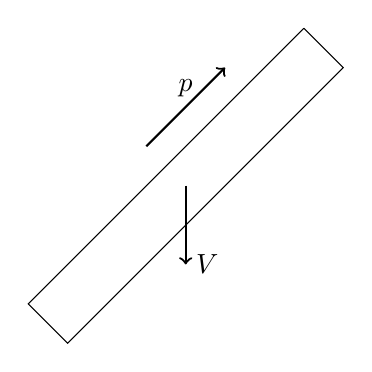
\begin{tikzpicture}
			\draw (1.5,2) -- (2, 1.5) -- (-1.5,-2) -- (-2,-1.5) -- (1.5, 2);
			\draw[thick,->] (0,0) -- (0,-1) node[right] {$\symbf{V}$};
			\draw[thick,->] (-0.5,0.5) -- (0.5,1.5) node[midway,above]
			{$\symbf{p}$};
		\end{tikzpicture}
	\end{center}

	If the rod falls perpendicular to its velocity (broadside) then $\symbf{p} \cdot
	\symbf{V} = 0$ so
	\begin{equation}
		\symbf{f} = \frac{4\pi\mu}{\log \frac{1}{\varepsilon}} \symbf{V},
		\hspace{2em} \symbf{F} = \frac{8\pi\mu L}{\log
		\frac{1}{\varepsilon}}\symbf{V}
	\end{equation}

	If the rod falls parallel to its velocity (lengthwise), we have
	$(\symbf{p}\cdot\symbf{V})\symbf{p} = \symbf{V}$ so
	\begin{equation}
		\symbf{f} = \frac{2\pi\mu}{\log \frac{1}{\varepsilon}} \symbf{V},
		\hspace{2em} \symbf{F} = \frac{4\pi\mu L}{\log
		\frac{1}{\varepsilon}}\symbf{V}
	\end{equation}

	\begin{enumerate}
		\item The rod falls lengthwise only twice as fast as broadside.
		\item The drag $\symbf{F}$ scales with $L$, not $\varepsilon R$, apart
			from $\log \frac{1}{\varepsilon}$, c.f. $\symbf{F} = 6\pi\mu a
			\symbf{U}$ for a sphere.
		\item Finite length more important than inertia if $\varepsilon =
			\frac{a}{L} \gg \text{Re}$.
		\end{enumerate}
\end{eg}

\begin{eg}
	Swimming flagellum. 
	
	\begin{center}
		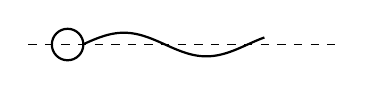
\begin{tikzpicture}
			\draw[dashed] (-2,0) -- (2,0);
			\draw[thick] (-1.5,0) circle (0.2);
			\draw[thick] plot[smooth,domain=-1.3:1,samples=100,variable=\x]
			({\x},{0.15*sin(3*(deg(\x)-45))});
		\end{tikzpicture}
	\end{center}
			
	Suppose the centreline is
	\begin{equation}
		\symbf{X}(s) = (-Ut+s, a\cos(ks-\omega t))
	\end{equation}
	i.e. a linearised wave with $a k \ll 1$. Then
	\begin{align}
		\symbf{V}(s) &= (-U, a\omega\sin(ks-\omega t)) \\
		\X'(s) &= (1, -ak\sin(ks-\omega t))
	\end{align}
	Write $S = \sin(ks-\omega t)$. Slender-body theory gives
	\begin{align}
		\symbf{f} &= \frac{4\pi\mu}{\log \frac{1}{\varepsilon}} \begin{pmatrix} 1-
			\frac{1}{2} & \frac{1}{2}akS \\ \frac{1}{2} akS & 1-
		\frac{1}{2}(akS)^2 \end{pmatrix} \begin{pmatrix} -U \\ a\omega S
		\end{pmatrix} \\
		&= \frac{4\pi \mu}{\log \frac{1}{\varepsilon}}\begin{pmatrix}
		-\frac{1}{2}U + \frac{1}{2}a^2k\omega S^2 \\ -\frac{1}{2}akUS + a\omega S
	\end{pmatrix}
	\end{align}
	Time averaging $\symbf{f}$ gives
	\begin{equation}
		\langle \symbf{f}\rangle = \frac{2\pi\mu}{\log \frac{1}{\varepsilon}}
	\begin{pmatrix} -U + \frac{1}{2}a^2k\omega \\ \end{pmatrix}
	\end{equation}
	There is no net force on the body, therefore $\langle \symbf{f}\rangle = 0$
	which implies $U = \frac{1}{2}a^2k\omega$.
\end{eg}

\lecture{2/11/20}
\subsection{Marangoni Flows}
The surface tension $\gamma$ between two immiscible fluids depends on the
fluids properties;
\begin{itemize}
	\item temperature - $\gamma$ decreases as $T$ increases. For water,
		$\inv{\gamma}\frac{\diffd \gamma}{\diffd T} \sim -\frac{1}{50 K}$. For
		example, \emph{Marangoni convection}. Heat applied to a fluid with
		surface tension generates circulation:
		\begin{center}
			\begin{tikzpicture}
				\draw (-3, 2) -- (-3, 0) -- (3, 0) -- (3, 2);
				\draw[red] (0, -1) node {heat};
				\draw[red,->] (0, -0.8) -- (0, -0.2);
				\draw[red,->] (0.5, -0.8) -- (0.5, -0.2);
				\draw[red,->] (-0.5, -0.8) -- (-0.5, -0.2);
				\draw plot [smooth] coordinates {(-3,1.4) (-2, 1.3) (-1,
				1) (0, 0.9) (1, 1) (2, 1.3) (3, 1.4)};
				\draw[blue] (0, 1.75) node{high $T$};
				\draw[blue] (0, 1.4) node{low $\gamma$};
				\draw[blue,->] (2, 0.7) [partial ellipse = 180:-90:0.7 and 0.35];
				\draw[blue,->] (-2, 0.7) [partial ellipse = 0:270:0.7 and 0.35];
				\draw[blue] (2.35, 2.05) node{low $T$};
				\draw[blue] (2.35, 1.7) node{high $\gamma$};
				\draw[red,thick,->] (0.7, 0.95) -- (2, 1.35)
				node[midway,above] {stress};
				\draw[red,thick,->] (-0.7, 0.95) -- (-2, 1.35)
				node[midway,above] {stress};
			\end{tikzpicture}
		\end{center}
	\item concentration of surfactants (surface active agents) - usually
		$\gamma$ decreases as the concentration $C$ increases. For example,
		detergent molecules spread over a surface. Detergent molecules have
		hydrophobic tails and hydrophilic heads.
		\begin{center}
			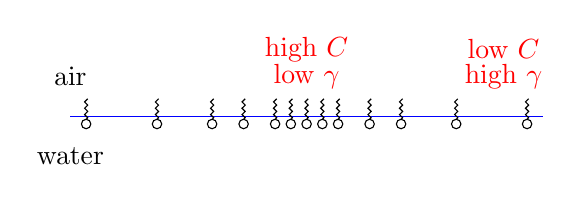
\begin{tikzpicture}
				\draw[blue] (-3, 0) -- (3, 0);
				\draw (-3, 0.5) node {air};
				\draw (-3, -0.5) node {water};
				\draw (0, -0.1) circle (0.06);
				\draw plot[smooth,tension=.5] coordinates {(0, -0.04) (0.02,
				-0.02) (0, 0) (-0.02, 0.02) (0, 0.04) (0.02, 0.06) (0, 0.08)
				(-0.02, 0.1) (0, 0.12) (0.02, 0.14) (0, 0.16) (-0.02, 0.18) (0,
				0.2) (0.02, 0.22)};
				\begin{scope}[shift={(0.2,0)}]
				\draw (0, -0.1) circle (0.06);
				\draw plot[smooth,tension=.5] coordinates {(0, -0.04) (0.02,
				-0.02) (0, 0) (-0.02, 0.02) (0, 0.04) (0.02, 0.06) (0, 0.08)
			(-0.02, 0.1) (0, 0.12) (0.02, 0.14) (0, 0.16) (-0.02, 0.18) (0,
		0.2) (0.02, 0.22)};
				\end{scope}
				\begin{scope}[shift={(0.4,0)}]
				\draw (0, -0.1) circle (0.06);
				\draw plot[smooth,tension=.5] coordinates {(0, -0.04) (0.02,
				-0.02) (0, 0) (-0.02, 0.02) (0, 0.04) (0.02, 0.06) (0, 0.08)
			(-0.02, 0.1) (0, 0.12) (0.02, 0.14) (0, 0.16) (-0.02, 0.18) (0,
		0.2) (0.02, 0.22)};
				\end{scope}
				\begin{scope}[shift={(0.8,0)}]
				\draw (0, -0.1) circle (0.06);
				\draw plot[smooth,tension=.5] coordinates {(0, -0.04) (0.02,
				-0.02) (0, 0) (-0.02, 0.02) (0, 0.04) (0.02, 0.06) (0, 0.08)
			(-0.02, 0.1) (0, 0.12) (0.02, 0.14) (0, 0.16) (-0.02, 0.18) (0,
		0.2) (0.02, 0.22)};
				\end{scope}
				\begin{scope}[shift={(1.2,0)}]
				\draw (0, -0.1) circle (0.06);
				\draw plot[smooth,tension=.5] coordinates {(0, -0.04) (0.02,
				-0.02) (0, 0) (-0.02, 0.02) (0, 0.04) (0.02, 0.06) (0, 0.08)
			(-0.02, 0.1) (0, 0.12) (0.02, 0.14) (0, 0.16) (-0.02, 0.18) (0,
		0.2) (0.02, 0.22)};
				\end{scope}
				\begin{scope}[shift={(1.9,0)}]
				\draw (0, -0.1) circle (0.06);
				\draw plot[smooth,tension=.5] coordinates {(0, -0.04) (0.02,
				-0.02) (0, 0) (-0.02, 0.02) (0, 0.04) (0.02, 0.06) (0, 0.08)
			(-0.02, 0.1) (0, 0.12) (0.02, 0.14) (0, 0.16) (-0.02, 0.18) (0,
		0.2) (0.02, 0.22)};
				\end{scope}
				\begin{scope}[shift={(2.8,0)}]
				\draw (0, -0.1) circle (0.06);
				\draw plot[smooth,tension=.5] coordinates {(0, -0.04) (0.02,
				-0.02) (0, 0) (-0.02, 0.02) (0, 0.04) (0.02, 0.06) (0, 0.08)
			(-0.02, 0.1) (0, 0.12) (0.02, 0.14) (0, 0.16) (-0.02, 0.18) (0,
		0.2) (0.02, 0.22)};
				\end{scope}
				\begin{scope}[shift={(-0.2,0)}]
				\draw (0, -0.1) circle (0.06);
				\draw plot[smooth,tension=.5] coordinates {(0, -0.04) (0.02,
				-0.02) (0, 0) (-0.02, 0.02) (0, 0.04) (0.02, 0.06) (0, 0.08)
			(-0.02, 0.1) (0, 0.12) (0.02, 0.14) (0, 0.16) (-0.02, 0.18) (0,
		0.2) (0.02, 0.22)};
				\end{scope}
				\begin{scope}[shift={(-0.4,0)}]
				\draw (0, -0.1) circle (0.06);
				\draw plot[smooth,tension=.5] coordinates {(0, -0.04) (0.02,
				-0.02) (0, 0) (-0.02, 0.02) (0, 0.04) (0.02, 0.06) (0, 0.08)
			(-0.02, 0.1) (0, 0.12) (0.02, 0.14) (0, 0.16) (-0.02, 0.18) (0,
		0.2) (0.02, 0.22)};
				\end{scope}
				\begin{scope}[shift={(-0.8,0)}]
				\draw (0, -0.1) circle (0.06);
				\draw plot[smooth,tension=.5] coordinates {(0, -0.04) (0.02,
				-0.02) (0, 0) (-0.02, 0.02) (0, 0.04) (0.02, 0.06) (0, 0.08)
			(-0.02, 0.1) (0, 0.12) (0.02, 0.14) (0, 0.16) (-0.02, 0.18) (0,
		0.2) (0.02, 0.22)};
				\end{scope}
				\begin{scope}[shift={(-1.2,0)}]
				\draw (0, -0.1) circle (0.06);
				\draw plot[smooth,tension=.5] coordinates {(0, -0.04) (0.02,
				-0.02) (0, 0) (-0.02, 0.02) (0, 0.04) (0.02, 0.06) (0, 0.08)
			(-0.02, 0.1) (0, 0.12) (0.02, 0.14) (0, 0.16) (-0.02, 0.18) (0,
		0.2) (0.02, 0.22)};
				\end{scope}
				\begin{scope}[shift={(-1.9,0)}]
				\draw (0, -0.1) circle (0.06);
				\draw plot[smooth,tension=.5] coordinates {(0, -0.04) (0.02,
				-0.02) (0, 0) (-0.02, 0.02) (0, 0.04) (0.02, 0.06) (0, 0.08)
			(-0.02, 0.1) (0, 0.12) (0.02, 0.14) (0, 0.16) (-0.02, 0.18) (0,
		0.2) (0.02, 0.22)};
				\end{scope}
				\begin{scope}[shift={(-2.8,0)}]
				\draw (0, -0.1) circle (0.06);
				\draw plot[smooth,tension=.5] coordinates {(0, -0.04) (0.02,
				-0.02) (0, 0) (-0.02, 0.02) (0, 0.04) (0.02, 0.06) (0, 0.08)
			(-0.02, 0.1) (0, 0.12) (0.02, 0.14) (0, 0.16) (-0.02, 0.18) (0,
		0.2) (0.02, 0.22)};
				\end{scope}
				\draw[red] (0, 0.85) node{high $C$};
				\draw[red] (0, 0.5) node{low $\gamma$};
				\draw[red] (2.5, 0.85) node{low $C$};
				\draw[red] (2.5, 0.5) node{high $\gamma$};
			\end{tikzpicture}
			\qquad
			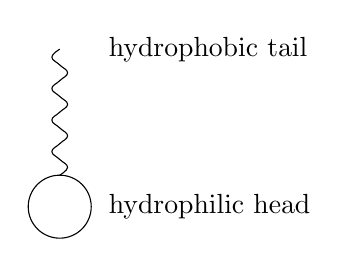
\begin{tikzpicture}
				\draw (0,0) circle (0.4);
				\draw plot[smooth,tension=.75] coordinates {(0,0.4) (0.1, 0.5)
				(0, 0.6) (-0.1, 0.7) (0, 0.8) (0.1, 0.9) (0, 1) (-0.1, 1.1)
			(0, 1.2) (0.1, 1.3) (0, 1.4) (-0.1, 1.5) (0, 1.6) (0.1, 1.7) (0,
		1.8) (-0.1, 1.9) (0, 2)};
		\draw (0.5, 2) node[right] {hydrophobic tail};
		\draw (0.5, 0) node[right] {hydrophilic head};
			\end{tikzpicture}
		\end{center}
		Another example is alcohol in water; `wine tears' creep up the side to
		form a rim on the meniscus due to high surface tension due to
		evaporating alcohol decreasing concentration.
		\begin{center}
			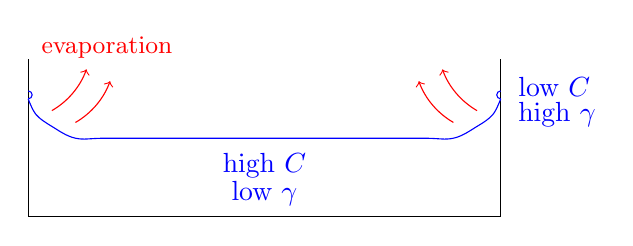
\begin{tikzpicture}
				\draw (-3, 2) -- (-3, 0) -- (3, 0) -- (3, 2);
				\draw[blue] plot[smooth,tension=.6] coordinates {(-3, 1.5) (-2.9,
				1.3) (-2.7, 1.15) (-2.4, 1) (-2, 1) (-1, 1) (0,1) (1,1) (2,1)
				(2.4, 1) (2.7, 1.15) (2.9, 1.3) (3, 1.5)};
				\draw[blue] (-3, 1.5) arc (-90:90:0.05);
				\draw[blue] (3, 1.5) arc (270:90:0.05);
				\draw[red,->] (-2.4, 1.2) arc (-60:-20:1);
				\draw[red,->] (-2.7, 1.35) arc (-60:-20:1);
				\draw[red] (-2, 2.15) node {\small evaporation};
				\draw[red,->] (2.4, 1.2) arc (240:200:1);
				\draw[red,->] (2.7, 1.35) arc (240:200:1);
				\draw[blue] (3.1, 1.65) node[right] {low $C$};
				\draw[blue] (3.1, 1.3) node[right] {high $\gamma$};
				\draw[blue] (0,0.65) node {high $C$};
				\draw[blue] (0,0.3) node {low $\gamma$};
			\end{tikzpicture}
		\end{center}
\end{itemize}

\subsubsection{Boundary conditions}
Surface tension can be represented by a surface stress (in $N \cdot m^{-1}$,
derived from a surface energy in $J \cdot m^{-2}$) acting isotropically across
lines in the surface with stress tensor
\begin{equation}
	\symbfsf{\sigma}^s = \gamma \left( \symsf{I} - \symbf{n}\symbf{n}\right)
\end{equation}
The force balance on an arbitrary small area of the interface gives
\begin{equation}
	\nabla_s \cdot \symbfsf{\sigma}^s + \left[ \symbfsf{\sigma} \cdot
	\symbf{n}\right]^+_- = 0
\end{equation}
where $\symbf{n}$ points out of the fluid and $\nabla_S = \left(\symsf{I} -
\symbf{n}\symbf{n}\right) \cdot \nabla$ is the gradient operator in the surface.
Hence the jump in fluid stress is
\begin{align}
	\left[ \symbfsf{\sigma} \cdot \symbf{n}\right]^+_- &= -\nabla_s \cdot
	\gamma \left( \symsf{I} - \symbf{n}\symbf{n}\right)\\
		&= -\left( \symsf{I} - \symbf{n}\symbf{n}\right) \cdot \nabla_s \gamma + \gamma
	\left( \nabla_s \cdot \symbf{n}\right)\symbf{n} + \gamma \cancel{(\symbf{n}\cdot
	\nabla_S)} \symbf{n}\\
	&= -\nabla_s \gamma + \gamma \kappa \symbf{n}
\end{align}
The first term is the surface gradient of $\gamma$ and the second is tension
$\times$ curvature, where curvature is denoted by $\kappa \equiv \nabla_s
\cdot \symbf{n}$.

Equivalently, in perpendicular and parallel components we have
\begin{align}
	\left[ \symbf{n} \cdot \symbfsf{\sigma} \cdot \symbf{n}\right]^+_- &= \gamma
	\kappa \\
	\left[ \symbf{n} \times \symbfsf{\sigma} \cdot \symbf{n}\right]^+_- &= -\symbf{n}
	\times \nabla_s \gamma
\end{align}

\subsubsection{Thermophoresis}
An immiscible drop in a temperature gradient migrates from cold regions to
hot.

\begin{center}
	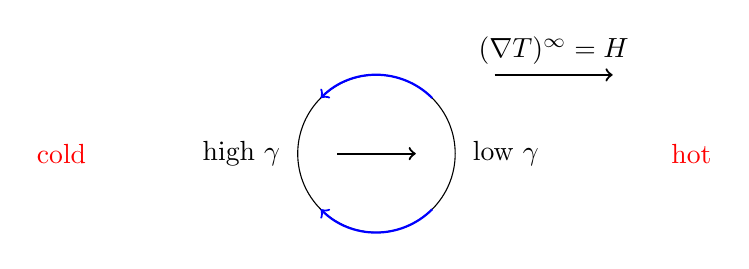
\begin{tikzpicture}
		\draw (0,0) circle (1);
		\draw[red] (-4, 0) node {cold};
		\draw[red] (4, 0) node {hot};
		\draw (1.1, 0) node[right] {low $\gamma$};
		\draw (-1.1, 0) node[left] {high $\gamma$};
		\draw[thick,blue,->] (0.7071,-0.7071) arc (-45:-135:1);
		\draw[thick,blue,->] (0.7071,0.7071) arc (45:135:1);
		\draw[thick,->] (-0.5, 0) -- (0.5, 0);
		\draw[thick,->] (1.5, 1) -- (3, 1) node[midway,above] {$(\nabla
		T)^\infty = H$};
	\end{tikzpicture}
\end{center}

Consider a scaling argument.  We have $\nabla T \sim H a \implies \nabla
\gamma \sim H a \gamma'$ where $\gamma' = \frac{\diffd \gamma}{\diffd T} < 0$.
The driving force $F$ from $\nabla \gamma$ acting across the equator length
$\sim a$ implies $F \sim H a^2 \gamma'$. Now $\sigma \sim \frac{\mu U}{a}$
acts over an area $\sim a^2$ to give viscous resistive force $\sim \mu U a$ (c.f.
drag on a sphere). Hence
\begin{equation}
	U \sim \frac{\gamma' H a}{\mu}
\end{equation}

Typical values are $H \sim 1^{\circ} C/cm, \gamma' \sim 1
\text{dyn}/cm/^{\circ} C, a \sim 10^{-2} cm, \rho \sim 1 g \cdot cm^{-3}, \nu
\sim 10^{-2} cm$. Therefore $U \sim 1 cm\cdot s^{-1}$.

\paragraph{Thermal problem.}
Consider the problem
\begin{equation}
	\frac{\partial T}{\partial t} + \symbf{u} \cdot \nabla T = \kappa \nabla^2 T
\end{equation}
with boundary conditions $\nabla T \to \symbf{H}$ as $\abs{\x} \to \infty$ and
\begin{equation}
	\left[ T\,\right]^+_- = \left[ k \symbf{n} \cdot \nabla T\,\right]^+_- = 0
	\hspace{2em} \text{on} \,\, \abs{\x} = a
\end{equation}
where $k$ is the conductivity ($\symbf{q} = -k \nabla T$) and $\kappa =
\frac{k}{\rho C_p}$ is the thermal diffusivity. Assume the \emph{Peclet}
number satisfies
\begin{equation}
	\text{Pe} = \frac{U a}{\kappa} = \frac{\text{advection}}{\text{diffusion}}
	\ll 1
\end{equation}

\lecture{4/11/20}
For $\text{Pe} \ll 1$, the problem reduces to solving $\nabla^2 T = 0$. Then,
for example, with an insulating drop ($k_1 \ll k_2$)
\begin{equation}
	T = T_0 + \symbf{H}\cdot\x \left(1+\frac{a^3}{2r^3}\right)
\end{equation}
and on $r =a$, $T = T_0 + \frac{3}{2}\symbf{H}\cdot\x$. Hence
\begin{equation}
	\gamma(T) = \gamma_0 + \gamma' (T-T_0) = \gamma_0 + \frac{3}{2}\gamma'
	\symbf{H}\cdot\x
\end{equation}

\paragraph{Fluid problem.}
The flow is driven by an interfacial force density 
\begin{align}
	\symbf{f}_s &= \symbfsf{\sigma}_1 \cdot \symbf{n} - \symbfsf{\sigma}_2 \cdot
	\symbf{n} \\
	&= \nabla_s \gamma - \gamma \symbf{n}\nabla_s \cdot \symbf{n} \\
	&= \left( \symsf{I}-\symbf{n}\symbf{n}\right) \cdot \frac{3}{2}\gamma'
	\symbf{H} - \frac{2}{a} \left( \gamma_0 + \frac{3}{2}\gamma'
	\symbf{H}\cdot\x\right)\symbf{n} \\
	&= -\frac{2}{a}\gamma_0 \symbf{n} + \frac{3}{2}\gamma'
	\symbf{H}\left(\symsf{I}-3\symbf{n}\symbf{n}\right)
\end{align}
where the second term drives the motion. For the simple case of equal
viscosities, $\lambda = 1$,
\begin{align}
	\symbf{u}(\y) &= \int_{r=a} \symsf{J}(\y-\x) \cdot \symbf{f}_s(\x) \cdot
	\diffd S \\
	&= \frac{3\gamma'}{16 \pi \mu} \symbf{H} \cdot \int \left(\symsf{I} - 3
	\symbf{n}\symbf{n}\right) \cdot \left( \frac{\symsf{I}}{R} +
	\frac{\symbf{R}\symbf{R}}{R^3}\right) \, \diffd S \hspace{1em}
	\text{where} \, \, \, \symbf{R} = \y - \x \\
	&= \frac{3 \gamma' a}{16 \pi \mu} \symbf{H} \cdot \symsf{G}(\y/a)
\end{align}
where, by symmetry of the integral and dimensions,
\begin{equation}
	\symsf{G} = \alpha(r/a) \symsf{I} + \beta(r/a)
	\hat{\symbf{y}} \hat{\symbf{y}}
\end{equation}
and $\hat{\symbf{y}} = \symbf{y}/a$. To determine the functions $\alpha,
\beta$ one can evaluate $G_{ii} = 3\alpha + \beta$ and $\hat{y}_i G_{ij}
\hat{y}_j = \alpha + \beta$. 

Now $\symbf{u} \cdot \hat{\symbf{y}} = \frac{3\gamma' a}{16 \pi \mu} (\alpha+\beta)
\symbf{H}\cdot\hat{\symbf{y}}$ which shows the spherical drop remains
spherical and translates with velocity
\begin{equation}
	\symbf{U} = \frac{3 \gamma' a}{16 \pi \mu} \left( \alpha(1) +
	\beta(1)\right) = -\frac{1}{5} \frac{a}{\mu} \gamma \symbf{H}
\end{equation}

\subsubsection{Surfactant effects}
The concentration $C$ in a small material area of interface $\delta $ changes
due to
\begin{enumerate}
	\item surface diffusion with flux $- D_s \nabla_s C$, where $D_s \sim
		10^{-9} m^2 s^{-1}$ typically
	\item absorbtion from the bulk fluid, if soluble, with rate $-k(C-C_0)$
		from chemical equilibrium and (linearised) kinetics $k \sim 10^3
		s^{-1}$
	\item change of area $\Delta (\delta A\, C) = 0 \implies \Delta C =
		-\frac{C}{\delta A} \Delta \delta A$. To get material
		$\frac{\diffd}{\diffd t} \delta A$, consider a material volume
		\begin{center}
			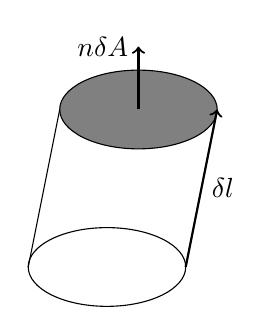
\begin{tikzpicture}
				\draw (0,0) ellipse (1 and 0.5);
				\draw[fill=gray] (.4,2) ellipse (1 and 0.5);
				\draw[thick,->] (1,0) -- (1.4, 2) node[midway,right]
				{$\symbf{\delta l}$};
				\draw (-1,0) -- (-0.6, 2);
				\draw[thick,->] (.4, 2) -- (.4, 2.8) node[left] {$\symbf{n}\delta A$};
			\end{tikzpicture}
		\end{center}
		Now $\delta V = \symbf{\delta l} \cdot \symbf{n} \delta A$. Hence
		\begin{equation}
			\frac{\diffd}{\diffd t} \delta V = \frac{\diffd}{\diffd t}
			\left[\symbf{\delta l}\right] \cdot \symbf{n} \delta A + \symbf{\delta l} \cdot
			\frac{\diffd}{\diffd t}\left[ \symbf{n} \delta A\right]
		\end{equation}
		We have $\frac{\diffd}{\diffd t} \delta V = \delta V \nabla \cdot
		\symbf{u}$ and $\frac{\diffd}{\diffd t} \symbf{\delta l} =
		(\symbf{\delta l} \cdot \nabla) \symbf{u}$ which, since $\symbf{\delta
		l}$ is arbitrary, gives
		\begin{equation}
			\frac{\diffd}{\diffd t} \left[ \symbf{n} \delta A \right] = \left(
			\symsf{I} \nabla \cdot \symbf{u} - \nabla \symbf{u} \right) \cdot
			\symbf{n} \delta A
		\end{equation}
		Taking the dot product with $\symbf{n}$ and noting $\symbf{n} \cdot
		\dot{\symbf{n}} = 0$ we have
		\begin{align}
			\frac{\diffd}{\diffd t} \delta A &= \left( \nabla \cdot \symbf{u}
			- \symbf{n} \symbf{n} : \nabla \symbf{u}\right) \delta A \\
			&= \nabla_s \cdot \symbf{u} \delta A \\
			&= \delta A \nabla_s \cdot \left[ \symbf{u}_s + (\symbf{u}\cdot
			\symbf{n})\symbf{n}\right] \\
			&= \delta A \left[ \nabla_s \cdot \symbf{u}_s +
			(\symbf{u}\cdot\symbf{n})\nabla_s \cdot \symbf{n} +
		\cancel{(\symbf{n}\cdot \nabla_s)(\symbf{u}\cdot\symbf{n})}\right]
		\end{align}
		Hence we have the \emph{transport equation}
		\begin{equation}
			\frac{\diffD C}{\diffD t} = -C \left[ \nabla_s \cdot \symbf{u}_s +
			(\symbf{u}\cdot\symbf{n})\symbf{n}\right] + D_s \nabla_s^2 C -
			k(C-C_0)
		\end{equation}
\end{enumerate}

\begin{eg}
	\hspace{1in}
	\begin{enumerate}
		\item \emph{Chemophoresis} -- migration in a background concentration
			gradient $\nabla C^\infty$
		\item \emph{Rigidifcation of interfaces} -- for example flow past a
			bubble.
			\begin{center}
				\begin{tikzpicture}
					\draw[thick] (0,0) circle (1);
					\draw[blue,<-] plot[smooth,domain=-3:3,variable=\y]
					({0.6+exp(-0.5*\y*\y)},{\y});
					\draw[blue,<-] plot[smooth,domain=-3:3,variable=\y]
					({-0.6-exp(-0.5*\y*\y)},{\y});
					\draw[thick,->] (2.5, 0.3) -- (2.5, -0.3) node[right]
					{$\symbf{g}$};
					\draw[blue,<-] (0.5, 0) [partial ellipse = 0:360:0.3 and 0.6];
					\draw[blue,<-] (-0.5, 0) [partial ellipse = 180:-180:0.3 and 0.6];
					\draw[red,->] (-0.5, 0) [partial ellipse = -110:-180:0.4
					and 0.7];
					\draw[red,->] (0.5, 0) [partial ellipse = -70:0:0.4 and 0.7];
					\draw (-.8, -0.4) node[red,left] {\tiny $\gamma$ gradient};
					\draw (0, 0.8) node[red] {\tiny high $\gamma$};
					\draw (0, -0.8) node[red] {\tiny low $\gamma$};
					
					\begin{scope}[shift={(0,-1.3)}]
						\draw[fill] (0, 0.28) circle (0.06);
						\draw plot[smooth,tension=.5] coordinates {(0, -0.04) (0.02,
						-0.02) (0, 0) (-0.02, 0.02) (0, 0.04) (0.02, 0.06) (0, 0.08)
					(-0.02, 0.1) (0, 0.12) (0.02, 0.14) (0, 0.16) (-0.02, 0.18) (0,
				0.2) (0.02, 0.22)};
					\end{scope}
					\begin{scope}[shift={(0.2,-1.27)},rotate=10]
						\draw[fill] (0, 0.28) circle (0.06);
						\draw plot[smooth,tension=.5] coordinates {(0, -0.04) (0.02,
						-0.02) (0, 0) (-0.02, 0.02) (0, 0.04) (0.02, 0.06) (0, 0.08)
					(-0.02, 0.1) (0, 0.12) (0.02, 0.14) (0, 0.16) (-0.02, 0.18) (0,
				0.2) (0.02, 0.22)};
					\end{scope}
					\begin{scope}[shift={(-0.2,-1.27)},rotate=-10]
						\draw[fill] (0, 0.28) circle (0.06);
						\draw plot[smooth,tension=.5] coordinates {(0, -0.04) (0.02,
						-0.02) (0, 0) (-0.02, 0.02) (0, 0.04) (0.02, 0.06) (0, 0.08)
					(-0.02, 0.1) (0, 0.12) (0.02, 0.14) (0, 0.16) (-0.02, 0.18) (0,
				0.2) (0.02, 0.22)};
					\end{scope}
					\begin{scope}[shift={(0.4,-1.21)},rotate=20]
						\draw[fill] (0, 0.28) circle (0.06);
						\draw plot[smooth,tension=.5] coordinates {(0, -0.04) (0.02,
						-0.02) (0, 0) (-0.02, 0.02) (0, 0.04) (0.02, 0.06) (0, 0.08)
					(-0.02, 0.1) (0, 0.12) (0.02, 0.14) (0, 0.16) (-0.02, 0.18) (0,
				0.2) (0.02, 0.22)};
					\end{scope}
					\begin{scope}[shift={(-0.4,-1.21)},rotate=-20]
						\draw[fill] (0, 0.28) circle (0.06);
						\draw plot[smooth,tension=.5] coordinates {(0, -0.04) (0.02,
						-0.02) (0, 0) (-0.02, 0.02) (0, 0.04) (0.02, 0.06) (0, 0.08)
					(-0.02, 0.1) (0, 0.12) (0.02, 0.14) (0, 0.16) (-0.02, 0.18) (0,
				0.2) (0.02, 0.22)};
					\end{scope}
					\begin{scope}[shift={(-0.8,-1)},rotate=-40]
						\draw[fill] (0, 0.28) circle (0.06);
						\draw plot[smooth,tension=.5] coordinates {(0, -0.04) (0.02,
						-0.02) (0, 0) (-0.02, 0.02) (0, 0.04) (0.02, 0.06) (0, 0.08)
					(-0.02, 0.1) (0, 0.12) (0.02, 0.14) (0, 0.16) (-0.02, 0.18) (0,
				0.2) (0.02, 0.22)};
					\end{scope}
					\begin{scope}[shift={(0.8,-1)},rotate=40]
						\draw[fill] (0, 0.28) circle (0.06);
						\draw plot[smooth,tension=.5] coordinates {(0, -0.04) (0.02,
						-0.02) (0, 0) (-0.02, 0.02) (0, 0.04) (0.02, 0.06) (0, 0.08)
					(-0.02, 0.1) (0, 0.12) (0.02, 0.14) (0, 0.16) (-0.02, 0.18) (0,
				0.2) (0.02, 0.22)};
					\end{scope}
				\end{tikzpicture}
			\end{center}
			Flow produces a concentration gradient $\nabla C$, which produces
			a surface tension gradient $\nabla \gamma$, which produces an
			opposing flow. In practice, a small contamination has a big effect.
	\end{enumerate}
\end{eg}

\lecture{6/11/20}
A steady flow in the frame of the bubble has $\frac{\partial C}{\partial t} =
0$ and $\symbf{u} \cdot \symbf{n} = 0$. Consider a linearised calculation with
$C = C_0 + C'(x)$ where $C' \ll C_0$. Then the transport equation reduces to
\begin{equation}
	D_s \nabla^2 C' - kC' = C_0 \nabla_s \cdot \symbf{u}_s
\end{equation}
where the non-linear terms $C' \nabla_s \cdot \symbf{u}_s$ and $\symbf{u}_s
\cdot \nabla_s C'$ have been neglected. Note $k$ vanishes if the fluid is
insoluble. This is a linear problem in the rise
velocity $\symbf{U}$ and from spherical symmetry we deduce
\begin{equation}
	\symbf{u}_s = A \left( \symsf{I} - \symbf{n}\symbf{n}\right)\cdot\symbf{U}
\end{equation}
for some constant $A$ to be determined. To calculate $\nabla_s \cdot \symbf{u}_s$, note
\begin{align}
	\nabla_s \symbf{n} &= \left( \symsf{I} - \symbf{n}\symbf{n}\right)\cdot
	\nabla \frac{\x}{a} = \frac{1}{a} \left( \symsf{I} -
	\symbf{n}\symbf{n}\right) \\
	\nabla_s \cdot \symbf{n} &= \frac{2}{a} \\
	\implies \nabla_s \cdot \symbf{u}_s &= -A \left[ (\nabla_s \cdot
		\symbf{n})\symbf{n} +
		\cancel{(\symbf{n}\cdot\nabla_s)}\symbf{n}\right]\cdot\symbf{U} =
		-\frac{2}{a} A\symbf{U}\cdot\symbf{n}
\end{align}
using the curvature $\kappa = \frac{2}{a}$ for a sphere of radius $a$.
Guessing $C' \propto \symbf{U}\cdot\symbf{n}$, and since 
\begin{equation}
	\nabla_s^2(\symbf{U}\cdot\symbf{n}) = \nabla_s \cdot \left[
	\frac{1}{a}\left(\symsf{I}-\symbf{n}\symbf{n}\right)\cdot\symbf{U}\right]
	= -\frac{2}{a^2}\symbf{U}\cdot\symbf{n}
\end{equation}
we find 
\begin{equation}
	C' = \frac{2C_0 A \frac{\symbf{U}\cdot\symbf{n}}{a}}{k + 2\frac{D_s}{a^2}}
\end{equation}
Therefore the linearisation $C' \ll C_0$ is valid if $\frac{UA}{D_s} \ll 1$
(fast diffusion) or $\frac{U}{ka} \ll 1$ (fast adsorption). The problem is
completed by using a Papkovich-Neuber representation inside and outside the
droplet with boundary conditions
\begin{align}
	\symbf{u} \to -\symbf{U} \,\,\, \text{as}\,\,\, &r \to \infty \\
	\symbf{u} \,\,\,\text{finite at} \,\,\, &r = 0 \\
	\symbf{u}= \symbf{u}_s \,\,\, \text{at} \,\,\, &r = a^+_-\\
	\left[\symbf{n} \times \symbfsf{\sigma}\cdot\symbf{n}\right]^+_- =
	-\symbf{n} \times \nabla C' \frac{\diffd \gamma}{\diffd C} \,\,\,
	\text{at} \,\,\, &r = a
\end{align}

These are 5 conditions for 4 potentials and $A$. We find the drag on the
bubble is
\begin{equation}
	\symbf{F} = -4\pi \mu a \symbf{U} \left(
	\frac{\frac{3}{2}(\lambda^*+\lambda)+1}{\lambda^*+\lambda+1}\right)
\end{equation}
where
\begin{equation}
	\lambda^* = -\frac{\frac{1}{3}a C_0 \frac{\diffd \gamma}{\diffd C}}{(a^2 k
	+ 2D_s)\mu}
\end{equation}
Note as $\lambda^* \to \infty$ we get a `rigid' sphere.

\subsection{Deformation of droplets.}
To leading order, a small force-free droplet moves with the flow
$\symbf{u}^\infty$ and is deformed by the local gradient
$(\symbf{x}\cdot\nabla)\symbf{u}^\infty$ against the restoring action of
surface tension. We assume the background flow is composed of a straining
component with symmetric traceless $\symsf{E}$ and a rotational component with
angular velocity $\symbf{\Omega}$. Hence $\symbf{u} \to \symbf{\Omega} \times
\x + \symsf{E}\cdot\x$ as $\abs{\x} \to \infty$.

\begin{center}
	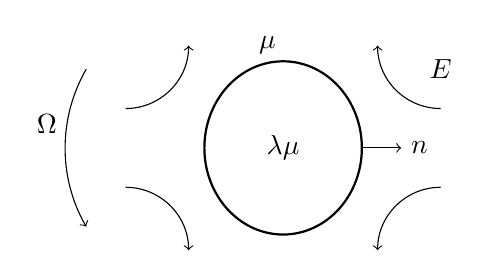
\begin{tikzpicture}
		\draw[thick] (0,0) ellipse (1 and 1.1);
		\draw[->] (-2, 0.5) arc (-90:0:0.8);
		\draw[->] (-2, -0.5) arc (90:0:0.8);
		\draw[->] (2, 0.5) arc (-90:-180:0.8);
		\draw[->] (2, -0.5) arc (90:180:0.8);
		\draw (2, 1) node {$\symsf{E}$};
		\draw (0,0) node {$\lambda \mu$};
		\draw (-0.2, 1.3) node {$\mu$};
		\draw[->] (1,0) -- (1.5, 0) node[right] {$\symbf{n}$};
		\draw[->] (-2.5,1) arc (150:210:2);
		\draw (-3, 0.3) node {$\symbf{\Omega}$};
	\end{tikzpicture}
\end{center}

The importance of viscous stress vs. surface tension is characterised by the
\emph{capillary number} $\text{Ca}$ where 
\begin{equation}
	\frac{\text{viscous stresses}}{\text{surface tension}} \sim \frac{\mu
	E}{\gamma/a} = \text{Ca} = \frac{\mu U}{\gamma}
\end{equation}

\subsubsection{Small deformations}
Here we consider $\text{Ca} \ll 1$ and a droplet with small deformation in a
pure strain flow $\symbf{u}^\infty = \symsf{E}\cdot\x$. Deformation is due to
symmetric traceless $\symsf{E}$. Hence for small (linearised) deformations we
expect (to first order in $\symsf{D}$)
\begin{equation}
	r= a\left[ 1 + \frac{\x \cdot \symsf{D}\cdot\x}{r^2}\right]
\end{equation}
where $\symsf{D}$ is symmetric, traceless (from volume conservation), and
$\mathcal{O}(\text{Ca})$. The surface normal is then
\begin{align}
	\symbf{n} &= \nabla \left( r - a\left[1 + \frac{\x \cdot
\symsf{D}\cdot\x}{r^2}\right]\right) \\
&= \frac{\x}{r} - 2a \left( \frac{\symsf{D}\cdot\x}{r^2} -
\frac{(\x\cdot\symsf{D}\cdot\x)\x}{r^4}\right) + \mathcal{O}(\symsf{D}^2)
\end{align}

Note $\abs{\symbf{n}} =1$ to $\mathcal{O}(\symsf{D}^2)$ as required. Also,
$\abs{\symbf{n}} = 1$ implies $\symbf{n}\cdot(\symbf{n}\cdot\nabla)\symbf{n} =
0$. Hence 
\begin{align}
	\nabla_s \cdot \symbf{n} &= \nabla \cdot \symbf{n} \\
		&= \frac{2}{r} + 6a \left.\frac{\x \cdot \symsf{D}\cdot\x}{r^4}\right|_s \\ 
	 &= \frac{2}{a} + 4\frac{\x \cdot \symsf{D}\cdot\x}{a^3} +
	\mathcal{O}(\symsf{D}^2)
\end{align}

\lecture{9/11/20}
To solve the problem, use a Papkovich-Neuber solution with
\begin{align}
	&\chi = \frac{1}{2} \x \cdot \symsf{E}\cdot\x + \frac{a^5}{3}
	\symsf{Q}:\nabla\nabla\inv{r}, &&\symbf{\Phi} = \frac{a^2}{3}
	\symsf{P}\cdot \nabla \inv{r} && r > a \\
	&\chi = \frac{1}{2}\x\cdot\symsf{e}\cdot\x, && \symbf{\Phi} =
	\frac{r^7}{6a^2} \symsf{p}:\nabla\nabla\nabla\inv{r} && r < a
\end{align}
where
\begin{itemize}
	\item the second rank tensors $\symsf{P},\symsf{Q},\symsf{p},\symsf{e}$
		are linearly dependent on $\symsf{D}, \symsf{E}$, and hence are all
		symmetric and traceless;
	\item the use of $\chi$ is forced by strain; the contribution of
		$\symsf{Q}$ to $\chi$ is equivalent to $\symbf{\Phi} = \frac{a^5}{r^5}
		\symsf{Q}:\nabla\nabla\nabla\inv{r}$;
	\item the coefficients are used to get the dimensions correction and to
		reduce numerical factors.
\end{itemize}

The fluid velocity is then
\begin{equation}
	\symbf{u} = \begin{cases}
		\symsf{e}\cdot\x + \left(\frac{5r^2}{a^2}\symsf{p}\cdot\x -
		\frac{2}{a^2} (\x\cdot\symsf{p}\cdot\x)\x\right) & \text{inside} \\
		\symsf{E}\cdot\x + \frac{a^3}{r^5}(\x\cdot\symsf{P}\cdot\x)\x + \left(
			\frac{2a^5}{r^5}\symsf{Q}\cdot\x -
			\frac{5a^5}{r^7}(\x\cdot\symsf{Q}\cdot\x)\x\right) &
			\text{outside}
	\end{cases}
\end{equation}
and similar expressions for $\symbfsf{\sigma}\cdot\symbf{n}$ on $r=a$ for
linearised BCs. Our boundary conditions are continuity of normal velocity;
continuity of tangential velocity; continuity of tangential stress; and jump
in normal stress equal to $\frac{2\gamma}{\mu a} \symsf{D}$. The kinematic
boundary condition $\symbf{u}\cdot\symbf{n} = \dot{r} = a \symbf{n} \cdot
\dot{\symsf{D}}(t)\cdot\symbf{n}$ gives
\begin{equation}
	\frac{\diffd \symsf{D}}{\diffd t} = \frac{5}{2\lambda+3}\symsf{E} -
	\frac{\gamma}{\mu a}
	\frac{40(\lambda+1)}{(2\lambda+3)(19\lambda+16)}\symsf{D}
\end{equation}
which tends monotonically to a linearised state
\begin{equation}
	\symsf{D} = \frac{19\lambda+16}{8(\lambda+1)} \frac{\mu a}{\gamma}
	\symsf{E}
\end{equation}

\subsubsection{Larger deformations}
Experiments and numerics show that the deformation increases monotonically in
the capillary number $\text{Ca}$ up to a critical value
$\text{Ca}_{\text{crit}}$ where the drop breaks. This critical value of
$\text{Ca}$ depends on the flow type and viscosity ratio $\lambda$. Taylor
(1934) showed that large $\lambda$ drops do not break in a simple shear. Since
a simple shear flow is composed of rotation and strain, we find the drop
rotates nearly rigidly with angular velocity $\symbf{\Omega}$ and sees an
oscillating strain tensor $\symsf{E}$, with steady deformation $\sim
\frac{\text{Ca}}{\lambda}$. In pure strain, we find $\text{Ca}_{\text{crit}}
\sim \lambda^{-1/6}$ for small $\lambda$ and $\text{Ca}_{\text{crit}}$ tends
to $\sim 0.1$ as $\lambda \to \infty$. Large $\lambda$ drops just take longer
to extend and break. Small $\lambda$ drops (bubbles) are hard to break.

\paragraph{Large deformations at $\lambda \ll 1$.}
In experiment, we see drops extending axisymmetrically and forming pointed
ends. We assume the drop is defined by $r=R(z)$ with $-L \le z \le L$ and $L
\gg R_0$, the maximum width of the droplet.
\begin{center}
	\begin{tikzpicture}[scale=2]
	\draw[thick,smooth] plot [domain=-2.582:2.582] ({\x},{0.03*\x*\x-0.2});
	\draw[thick,smooth] plot [domain=-2.582:2.582] ({\x},{-0.03*\x*\x+0.2});
	\draw (0, 0.3) node {$r=R_0$};
	\draw[->] (0,0) -- (0, 0.2);
	\draw[dashed] (-3, 0) -- (3, 0);
	\draw (-2.8, -0.1) node {$z=-L$};
	\draw (2.8, -0.1) node {$z=L$};
	\draw (1.6, 0.25) node {$r=R(z)$};
	\draw[->] (1.3, 0) -- (1.3, 0.15);
	\draw[blue,<-] (2, 0.8) [partial ellipse = -90:-160:1 and 0.35];
	\draw[blue,<-] (-2, 0.8) [partial ellipse = -90:-20:1 and 0.35];
	\draw[blue,<-] (-2, -0.8) [partial ellipse = 90:20:1 and 0.35];
	\draw[blue,<-] (2, -0.8) [partial ellipse = 90:160:1 and 0.35];
\end{tikzpicture}
\end{center}

Since $\lambda \ll 1$, we neglect the shear stress exerted by the internal
flow, so that $u_z^{\text{ext}} = Ez \sim EL$. We start by neglecting pressure
gradients in the bubble: moving along the bubble with a material slice of the
external fluid, we see a circular hole of radius $R(z)$ collapsing with
velocity $E z \frac{\diffd R}{\diffd z}$ with strain rate $\sim
\frac{\text{velocity}}{r}$, due to a stress difference $\frac{\gamma}{R}$
between inside and out. Hence 
\begin{equation}
	\mu E \sim \frac{\gamma}{R_0} \implies \frac{a}{R_0} \sim \text{Ca}
\end{equation}
The volume constraint gives $R_0^2 L \sim a^3$ so that $\frac{L}{R_0} \sim
\text{Ca}^3$. The flow inside the drop is (nearly) Poiseuille, but with wall
velocity $Ez$ and no net flux. 
\begin{center}
	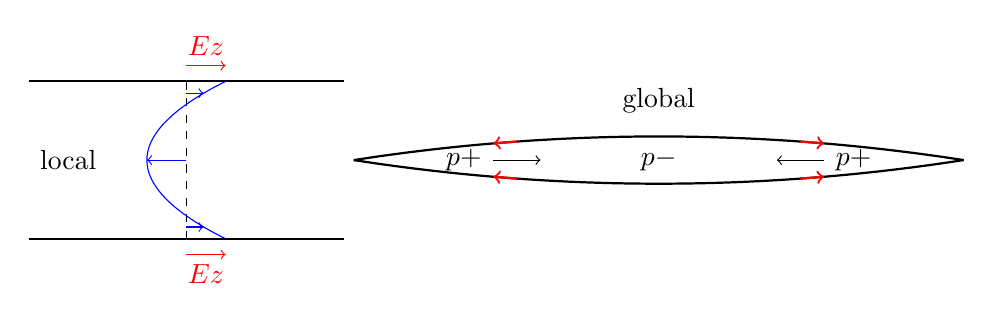
\begin{tikzpicture}
		\begin{scope}[shift={(-3,0)}]
		\draw[thick] (-2, 1) -- (2, 1);
		\draw[thick] (-2, -1) -- (2, -1);
		\draw[dashed] (0,1) -- (0,-1);
		\draw[smooth,blue] plot[domain=-1:1,variable=\y] ({\y*\y-0.5},{\y});
		\draw[blue,->] (0,0) -- (-0.5,0);
		\draw[blue,->] (0,0.85) -- (0.22, 0.85);
		\draw[blue,->] (0,-0.85) -- (0.22, -0.85);
		\draw[red,->] (0, 1.2) -- (0.5, 1.2) node[midway,above] {$Ez$};
		\draw[red,->] (0, -1.2) -- (0.5, -1.2) node[midway,below] {$Ez$};
		\draw (-1.5, 0) node {local};
		\end{scope}
		\begin{scope}[shift={(3,0)},scale=1.5]
		\draw (0,0.5) node {global};
		\draw[thick,smooth] plot [domain=-2.582:2.582] ({\x},{0.03*\x*\x-0.2});
		\draw[thick,smooth] plot [domain=-2.582:2.582] ({\x},{-0.03*\x*\x+0.2});
		\draw[->] (-1.4, 0) -- (-1, 0);
		\draw[->] (1.4,0) -- (1, 0);
		\draw (-1.65, 0) node {$p+$};
		\draw (1.65, 0) node {$p+$};
		\draw (0,0) node {$p-$};
		\draw[thick,red,<-] (-1.4, 0.1412) -- (-1.2, 0.1568);
		\draw[thick,red,<-] (-1.4, -0.1412) -- (-1.2, -0.1568);
		\draw[thick,red,<-] (1.4, 0.1412) -- (1.2, 0.1568);
		\draw[thick,red,<-] (1.4, -0.1412) -- (1.2, -0.1568);
		\end{scope}
	\end{tikzpicture}
\end{center}

To balance the pressure gradient we require 
\begin{equation}
	\frac{\Delta p}{L} \sim \frac{\lambda \mu E L}{R_0^2}
\end{equation}
This is possible provided $\Delta p \le \frac{\gamma}{R_0}$, i.e. $\lambda \ll
\frac{\gamma}{R_0 \mu E} \frac{R_0^2}{L^2}$. Note the factor $\gamma/R_0 \mu
E \sim 1$ so
\begin{equation}
	\lambda \ll \frac{R_0^2}{L^2} \sim \text{Ca}^{-6}
\end{equation}

\subsection{Rayleigh-Plateau Instability}
Consider small axisymmetric perturbations to the shape of a cylinder of one
fluid surrounded by another.
\begin{center}
	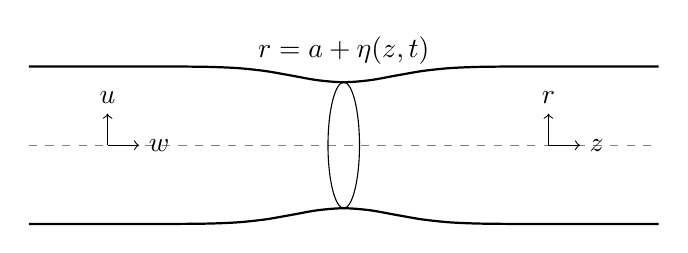
\begin{tikzpicture}[scale=2]
		\draw[thick,smooth] plot[domain=-2:2] ({\x},{0.5-0.1*exp(-5*\x*\x)});
		\draw[thick,smooth] plot[domain=-2:2] ({\x},{-0.5+0.1*exp(-5*\x*\x)});
		\draw[dashed,opacity=0.5] (-2,0) -- (2,0);
		\draw[->] (-1.5, 0) -- (-1.3, 0) node[below,right] {$w$};
		\draw[->] (-1.5, 0) -- (-1.5, 0.2) node[left,above] {$u$};
		\draw[->] (1.3, 0) -- (1.5, 0) node[below,right] {$z$};
		\draw[->] (1.3, 0) -- (1.3, 0.2) node[left,above] {$r$};
		\draw (0,0) ellipse (0.1 and 0.4);
		\draw (0,0.6) node {$r=a+\eta(z,t)$};
	\end{tikzpicture}
\end{center}

The cylinder has radius $r=a+\eta(z,t)$ with $\eta \ll a$ and $\eta_z \ll 1$.
The surface normal is
\begin{equation}
	\symbf{n} = (1,0,-\eta_z) + \mathcal{O}(\eta^2)
\end{equation}
Hence
\begin{equation}
	\nabla \cdot \symbf{n} = \frac{1}{r} - \eta_{zz} \approx
	\frac{1}{a}-\frac{\eta}{a^2} - \eta_{zz} + \mathcal{O}(\eta^2)
\end{equation}
\lecture{11/11/20}
The $\eta/a^2$ term accounts of azimuthal curvature and the $\eta_{zz}$ term
accounts for axial curvature. Consider disturbances of the form $\eta =
\hat{\eta} e^{st} \cos kz$. Then
\begin{equation}
	\nabla \cdot \symbf{n} = \frac{1}{a} - \frac{1-k^2 a^2}{a^2} \eta
\end{equation}
The disturbance is stabilised by axial curvature which acts to reduce the
disturbance, and is destabilised by azimuthal curvature which acts to
constrict the cylinder further.

\begin{center}
	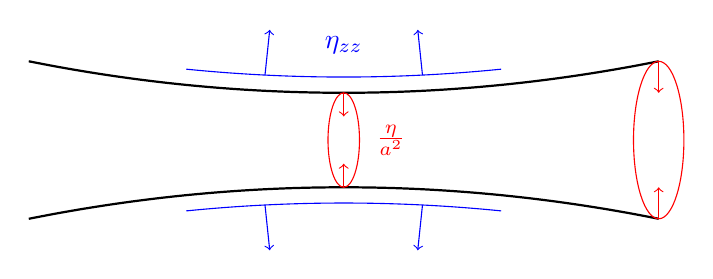
\begin{tikzpicture}[scale=2]
		\draw[thick,smooth] plot[domain=-2:2] ({\x},{0.3+0.05*\x*\x});
		\draw[thick,smooth] plot[domain=-2:2] ({\x},{-0.3-0.05*\x*\x});
		\draw[smooth,blue] plot [domain=-1:1] ({\x},{0.4+0.05*\x*\x});
		\draw[smooth,blue] plot [domain=-1:1] ({\x},{-0.4-0.05*\x*\x});
		\draw[red] (0,0) ellipse (0.1 and 0.3);
		\draw[red] (2, 0) ellipse (0.16 and 0.5);
		\draw[red,->] (0,0.3) -- (0, 0.15);
		\draw[red,->] (0,-0.3) -- (0, -0.15);
		\draw[red,->] (2,0.5) -- (2, 0.3);
		\draw[red,->] (2,-0.5) -- (2, -0.3);
		\draw[blue,->] (0.5, 0.4125) -- (0.47, 0.7);
		\draw[blue,->] (-0.5, 0.4125) -- (-0.47, 0.7);
		\draw[blue,->] (0.5, -0.4125) -- (0.47, -0.7);
		\draw[blue,->] (-0.5, -0.4125) -- (-0.47, -0.7);
		\draw[red] (0.3, 0) node {$\frac{\eta}{a^2}$};
		\draw[blue] (0, 0.6) node {$\eta_{zz}$};
	\end{tikzpicture}
\end{center}

The disturbance is unstable to long wavelengths with $k^2 a^2 < 1$. The growth
rate $s$ depends on the dynamics. The full case including inertia, internal
and external pressure, and internal and external viscosity is given by
Tomotika (1935). We will sketch the simple case of no inertia and no external
viscosity. The linearised boundary conditions are
\begin{align}
	\text{kinematic} \hspace{3em}\eta_t &= \left.u\right|_{r=a} \hspace{2em}
	\text{neglecting} \,\, w \eta_z \\
	 \implies \eta &= \frac{u}{s} \,\,\,\text{on}\,r=a \\ 
	 \text{dynamic}\hspace{1em}
	 \left[ \symbfsf{\sigma}\cdot\symbf{n}\right]_-^+ &= \gamma (\nabla \cdot
	 \symbf{n})\symbf{n} \\
	\symbfsf{\sigma}_{\text{out}} &= 0 
\end{align}
Hence the stress components are, on $r=a$,
\begin{align}
	\frac{\partial u}{\partial z} + \frac{\partial w}{\partial r} &= 0
																																				&&\text{tangential}\\
	\cancel{-p_0}-p + 2\mu \frac{\partial u}{\partial r} &= \gamma \left(
	\frac{1-k^2a^2}{a^2}\right) \frac{u}{s} - \cancel{\frac{\gamma}{a}}
	&&\text{normal}
\end{align}
where in the normal component the balanced terms $-p_0 = -\frac{\gamma}{a}$
are excluded since they play no role in the dynamics. To find the Stokes flow
inside the cylinder, we need the axisymmetric harmonic functions which are
proportional to $\cos kz$, derived by separation of variables. We have
\begin{align}
	\chi &= A I_0(kr) \cos kz \\
	\symbf{\Phi} &= (BI_1(kr) \cos  kz, 0,0)
\end{align}
where $I_0$ and $I_1$ are modified Bessel functions which are well behaved at
the origin. Note that the $\hat{\symbf{z}}$ component of $\symbf{\Phi}$
vanishes to avoid $w \propto z$ as we only want oscillatory motion in the $z$
direction. Note also that $I_0'(x) = I_1(x)$ and $xI_0 = (x I_x(x))'$. We find
\begin{align}
	u &= (AkI_1 + Bkr I_0 - 2BI_1) \cos kz \\
	w &= (-AkI_0 - Bkr I_1) \sin kz \\
	p &= 2 \mu B k I_0 \cos kz
\end{align}
Applying the boundary conditions yields the growth rate as
\begin{equation}
	s = \frac{\gamma}{2\mu a} (1-k^2 a^2) \frac{I_1(ka)^2}{k^2 a^2 I_0(ka)^2
	- (1+k^2 a^2) I_1(ka)^2}
\end{equation}
as derived by Lord Rayleigh (1892).

\begin{center}
	\begin{tikzpicture}
		\draw[thick,->] (-0.1,0) -- (5, 0) node[right] {$ka$};
		\draw[thick,->] (0, -1) -- (0,1.4) node[left] {$s$};
		\draw[blue,smooth] plot[domain=0:3.6] ({\x},{1.2+1/(\x-4)});
		\draw (0.1, 0.95) -- (-0.1, 0.95) node[left] {$\frac{\gamma}{6\mu a}$};
		\draw (3.16,0.1) -- (3.16, -0.1) node[below] {$1$};
	\end{tikzpicture}
\end{center}

\begin{enumerate}
	\item The most unstable disturbance has infinite wavelength since this
		minimises the internal deformation and we have ignored external drag.
		A cylindrical bubble in viscous fluid is also most unstable at
		infinite wavelengths, since it minimises external $\frac{\partial
		u}{\partial z}$ and ignores internal Poiseuille flow.
	\item If $0 < \lambda < \infty$ then the maximum $s$ is at finite $k$.
	\begin{center}
		\begin{tikzpicture}
				\draw[thick,->] (-0.1,0) -- (5, 0) node[right] {$ka$};
				\draw[thick,->] (0, -1) -- (0,1.4) node[left] {$s$};
				\draw (3.16,0.1) -- (3.16, -0.1) node[below] {$1$};
				\draw[blue,smooth] plot[tension=0.8] coordinates {(0,0) (0.5, 0.2) (1, 0.5)
				(1.5, 1) (2, 1.15) (2.5, 0.9) (3, 0.3)  (3.7, -1.2)};
			\end{tikzpicture}
		\end{center}
	\item Consider the scaling requierd to be able to neglect inertia. Suppose
		$ak = \mathcal{O}(1)$, then we have from the boundary conditions
		\begin{equation}
			\frac{\mu u}{a^2} \sim \frac{p}{a} \sim \frac{\gamma}{a^2},
			\hspace{2em} u \sim as 
		\end{equation}
		Thus we find the growth rate scales as $s \sim \frac{\gamma}{\mu a}$
		as we expected from the solution. If inertia is much smaller than
		viscous terms then we have
		\begin{equation}
			\rho u s \ll \frac{\mu u}{a^2} \implies \frac{\mu ^2}{\gamma \rho
			a} \gg 1
		\end{equation}
	\item There are interesting self-similar dynamics in the non-linear regime
		as the point of breakup is reached.
\end{enumerate}

\subsection{Long Thin Flows I: Lubrication Theory}
\label{ss:lube}
Here we consider thin flow with (at least one) effectively no-slip boundary.
Denote the fluid depth as $h$ and the horizontal lengthscale $L$. We assume $h
\ll L$.

\begin{center}
	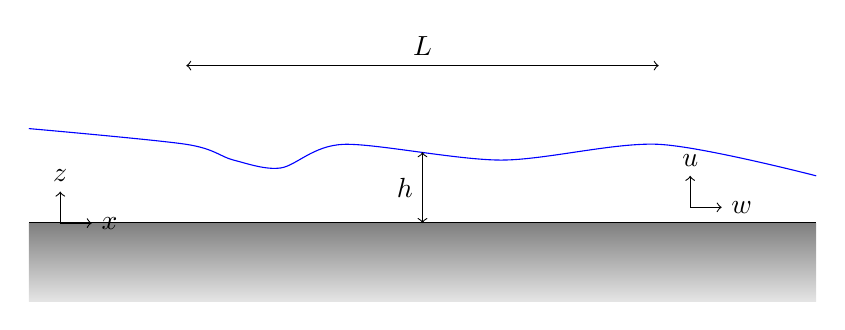
\begin{tikzpicture}[scale=2]
		\draw[thick] (0,0) -- (5, 0);
		\fill[middle color = gray, bottom color = gray!20] (0,0) -- (5,0) -- (5, -0.5) -- (0, -0.5);
		\draw[->] (4.2, 0.1) -- (4.4, 0.1) node[below,right] {$w$};
		\draw[->] (4.2, 0.1) -- (4.2, 0.3) node[left,above] {$u$};
		\draw[->] (0.2, 0) -- (0.4, 0) node[below,right] {$x$};
		\draw[->] (0.2, 0) -- (0.2, 0.2) node[left,above] {$z$};
		\draw[smooth,blue] plot coordinates {(0,0.6) (1, 0.5) (1.3, 0.4) (1.6,
		0.35) (2, 0.5) (3, 0.4) (4, 0.5) (5, 0.3)};
		\draw[<->] (2.5,0) -- (2.5, 0.45) node[midway, left] {$h$};
		\draw[<->] (1, 1) -- (4, 1) node[midway,above] {$L$};
	\end{tikzpicture}
\end{center}

Assume the velocity gradients satisfy $\partial_x \sim \frac{1}{L} \ll
\frac{1}{h} \sim \partial_z$. Consider the scalings for the governing
equations. From incompressibility we have
\begin{equation}
	\nabla \cdot \symbf{u} = 0 \implies \frac{u}{L} \sim \frac{w}{h} \implies
	w \ll u
\end{equation}
From Navier-Stokes we have
\begin{align}
	&\text{NS (steady)} && \rho (\symbf{u}\cdot\nabla)\symbf{u}\hspace{2em} =
	&&-\nabla p
	\hspace{2em}+ &&\mu \nabla^2 \symbf{u} &&\\
	  &\parallel \text{to boundary} &&\rho \frac{u^2}{L} &&\,\,\, \frac{p}{L} && \mu
	\left(\frac{u}{L^2}\right. + &&\left.\frac{u}{h^2}\right)\\
	&\implies &&\frac{u h}{\nu} \frac{h}{L} && \frac{p}{\left(\frac{\mu uL}{h^2}\right)}
	&&\frac{h^2}{L^2} && 1
\end{align}
Hence we can neglect inertia provided the \emph{modified Reynolds number}
$\frac{u h}{\nu} \frac{h}{L} \ll 1$. Note we can also approximate $\nabla^2$
by $\frac{\partial^2}{\partial z^2}$, and we expect $p \sim \frac{\mu u
L}{h^2}$ (cf. pipe flow). The component perpendicular to the boundary scales
as
\begin{align}
	&\text{NS (steady)} && \rho (\symbf{u}\cdot\nabla)\symbf{u}\hspace{2em} =
	&&-\nabla p
	\hspace{2em}+ &&\mu \nabla^2 \symbf{u} &&\\
		&\perp \text{to boundary} && \frac{\rho u w}{L} && \frac{p}{h} && \mu\left( \frac{w}{L^2}\right. +
								&&\left.  \frac{w}{h^2}\right)\\
					   &\implies && \left( \frac{u h}{\nu}\right)
	\frac{h^2}{L^2} && 1 && \frac{h^4}{L^4} +&&\frac{h^2}{L^2}
\end{align}
so at leading order we have $\frac{\partial p}{\partial z} = 0$, i.e. $p =
p(x,y,t)$ only. The flow in the thin layer is quasi-parallel to the boundary.
\lecture{13/11/20}
Let $\symbf{u} \equiv (u,v)$ and $\nabla \equiv (\partial_x, \partial_y)$
denote the parallel components of velocity and gradient. Our governing
equation is now
\begin{equation}
	\mu \frac{\partial^2 \symbf{u}}{\partial z^2} = \nabla p
\end{equation}
Define the \emph{depth-integrated parallel volume flux}
\begin{equation}
	\symbf{q} = \int_0^h \symbf{u} \, \diffd z
\end{equation}
Depth-integrated conservation of mass can then be written as
\begin{equation}
	\frac{\partial h}{\partial t} + \nabla \cdot \symbf{q} = 0
\end{equation}

Note on a curve surface $\nabla$ should be replaced by $\nabla_s$. These three
equations can be solved with various boundary conditions at $z=0,h$, or
equivalently $z=h_1, h_2$.

\subsubsection{Squeeze films}
Here we have prescribed velocity boundary conditions
\begin{align}
	\symbf{u} = \begin{cases} \symbf{U}_1 & z=0 \\ \symbf{U}_2 & z=h
	\end{cases}
\end{align}
Subject to these boundary conditions we find
\begin{align}
	\symbf{u} &= -\frac{\nabla p}{2\mu} z(h-z) + \symbf{U}_1 +
	(\symbf{U}_2-\symbf{U}_1) \frac{z}{h}\\
	\symbf{q} &= -\frac{h^3}{12\mu}\nabla p +
	\frac{h}{2}(\symbf{U}_1+\symbf{U}_2)
\end{align}

Applying mass conservation yields \emph{Reynold's (lubrication) equation}
\begin{equation}
	\frac{\partial h}{\partial t} = \frac{1}{12\mu} \nabla \cdot (h^3 \nabla
	p) - \frac{1}{2} \nabla \cdot h(\symbf{U}_1+\symbf{U}_2)
\end{equation}
Usually given the velocities, we first calculate the pressure field $p$ and
then the force as an integral of pressure over the surface.

\begin{eg}
	Rigid sphere settling towards a plane wall.
	\begin{center}
		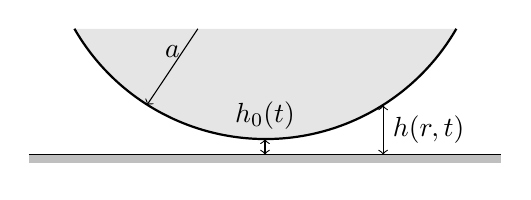
\begin{tikzpicture}
			\draw[thick,] (-3,0) -- (3, 0);
			\draw[thick,fill=gray!20] (-2.42, 1.6) arc (-150:-30:2.8);
			\draw[<->] (0,0) -- (0, 0.2) node [above] {$h_0(t)$};
			\draw[<->] (1.5,0) -- (1.5, 0.63) node[midway,right] {$h(r,t)$};
			\fill[gray!50] (-3,0) rectangle (3, -0.1);
			\draw[<-] (-1.5, 0.63) -- (-0.853,1.6) node[midway,above] {$a$};
		\end{tikzpicture}
	\end{center}
	The gap thickness is given by
	\begin{equation}
		h(r,t) = h_0(t) + \frac{r^2}{2a} + \mathcal{O}(\frac{r^4}{a^3})
	\end{equation}
	with $\partial_t h = \dot{h}_0 < 0$. By mass conservation (i.e. either
	integrate the mass conservation equation or consider flux across $r =\,
	$constant) we have
	\begin{equation}
		-\pi r^2 \dot{h}_0 \hat{\symbf{r}} = 2\pi r \symbf{q}(r)
	\end{equation}
	and for these rigid-rigid boundary conditions we solve to find
	\begin{align}
		\symbf{u} &= -\frac{1}{2\mu}\frac{\partial p}{\partial r} y(h-y)
		\hat{\symbf{r}} \\
		\symbf{q} &= -\frac{h^3}{12\mu} \frac{\partial p}{\partial r}
		\hat{\symbf{r}}
	\end{align}
	We can use the expression for $\symbf{q}$ and mass conservation to find
	$\frac{\partial p}{\partial r}$ and integrate to get
	\begin{equation}
		p(r,t) = \int^r \frac{6\mu \dot{h}_0 r}{h^3} \, \diffd r = -\frac{6
		\mu \dot{h}_0}{h_0^3} \int_r^\infty \frac{r}{(1+r^2/2ah_0)^3} \,
		\diffd r = p_\infty - \frac{3\mu \dot{h}_0 a}{h_0^2 (1+r^2/2ah_0)^2}
	\end{equation}
	Hence the force on the sedimenting sphere is
	\begin{equation}
		F = 2\pi \int_0^\infty (p-p_\infty) r \, \diffd r = -\frac{6\pi \mu
		a^2 \dot{h}_0}{h_0}
	\end{equation}
\end{eg}
\begin{eg}
	Hele-Shaw flow. A simple case of the above is $\symbf{U}_i = 0$ with $h$
	uniform and constant. Then
	\begin{align}
		\nabla^2 p &= 0 \\
		\symbf{q} &= -\frac{h^3}{12\mu} \nabla p
	\end{align}
	Boundary conditions on $p$ or $\symbf{q}\cdot\symbf{n}$ are needed. This
	set-up is often used to visualise flow past an object.
\end{eg}

\subsubsection{Free-surface flows}
Consider the boundary conditions
\begin{align}
	\symbf{u} &= 0 \hspace{1em} \text{on} \,\,\, z=0 \\
	\mu \frac{\partial \symbf{u}}{\partial z} &= 0 \hspace{1em} \text{on}
	\,\,\, z=h
\end{align}
Subject to these conditions, the solution is
\begin{align}
	\symbf{u} &= - \frac{\nabla p}{2\mu} z(2h-z) \\
	\symbf{q} &= -\frac{h^3}{3\mu} \nabla p	 \\
	\frac{\partial h}{\partial t} &= \frac{1}{3\mu} \nabla \cdot (h^3 \nabla
	p)
\end{align}
Usually, $p$ is specified, for example from gravity and surfacae tension $p =
\rho g (h-z) - \gamma \nabla^2 h$, from which $\frac{\partial h}{\partial t}$
is calculated.
\subsubsection{Marangoni flows}
Consider replacing the top rigid or free surface boundary condition with a
surface tension condition 
\begin{equation}
	\mu \frac{\partial \symbf{u}}{\partial z} = \nabla \gamma
\end{equation}
\begin{eg}
	Viscous drop approaching a plane wall.
	\begin{center}
		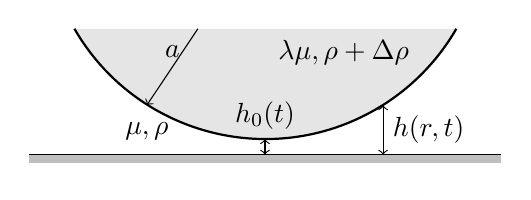
\begin{tikzpicture}
			\draw[thick,] (-3,0) -- (3, 0);
			\draw[thick,fill=gray!20] (-2.42, 1.6) arc (-150:-30:2.8);
			\draw[<->] (0,0) -- (0, 0.2) node [above] {$h_0(t)$};
			\draw[<->] (1.5,0) -- (1.5, 0.63) node[midway,right] {$h(r,t)$};
			\fill[gray!50] (-3,0) rectangle (3, -0.1);
			\draw[<-] (-1.5, 0.63) -- (-0.853,1.6) node[midway,above] {$a$};
			\draw (-1.5, 0.3) node{$\mu, \rho$};
			\draw (1, 1.3) node{$\lambda\mu, \rho+\Delta \rho$};
		\end{tikzpicture}
	\end{center}
	Assume to start with that
	\begin{enumerate}
		\item surface tension is present and keeps the drop spherical;
		\item $\lambda \gg 1$ so the drop is effectively rigid.
	\end{enumerate}
	Consider the following scalings. 
	\begin{align}
		L &\sim \sqrt{ah_0} &&\text{from geometry}\\
		\mu &\sim \frac{L}{h_0} \dot{h}_0 &&\text{from mass conservation}\\
		p &\sim \frac{\mu u L}{h_0^2} \sim \frac{\mu a}{h_0^2} \dot{h}_0
		  &&\text{from pipe flow}\\
		F &\sim p L^2 \sim \frac{\mu a^2}{h_0} \dot{h}_0 &&(\sim \Delta \rho g
		a^3 \,\,\, \text{if balancing weight})
	\end{align}
	From these we can check our assumptions.
	\begin{enumerate}
		\item High pressure in the middle of the gap deforms the drop by
			$\Delta h$ over lengthscale $L$. Then $p \sim \gamma \Delta
			\kappa$ and $\Delta \kappa \sim \frac{\Delta h}{L^2}$. Hence
			\begin{equation}
				\frac{\Delta h}{h_0} \sim \frac{p}{\gamma/a} \sim \frac{\mu
				\dot{h}_0}{\gamma} \frac{a^2}{h_0^2}
			\end{equation}
			Thus deformation is negligible if the capillary number $\text{Ca}
			\equiv \frac{\mu \dot{h}_0}{\gamma} \ll \frac{h_0^2}{a^2}$, or the
			\emph{Bond number} $\text{Bo} \equiv \frac{\Delta \rho g
			a^2}{\gamma} \ll \frac{h_0}{a}$. Note the Bond number indicates
			the importance of weight over capillary pressure. This requirement
			is eventually invalid as $h_0$ decreases.
		\item The shear stress $\sim \frac{\mu u}{h_0}$ in the gap drives flow
			$u_D$ in the drop over a lengthscale $L$.
			\begin{center}
				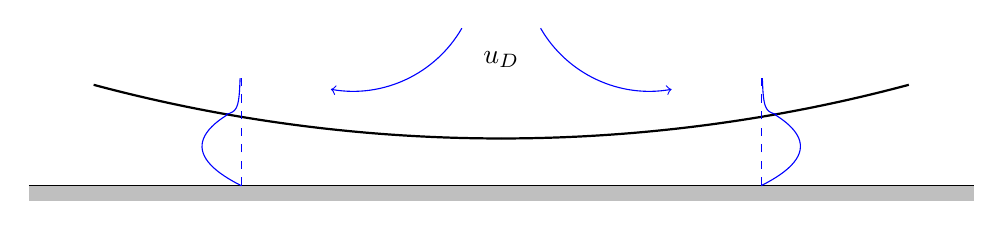
\begin{tikzpicture}[scale=2]
					\draw[thick] (-3,0) -- (3,0);
					\fill[gray!50] (-3,0) rectangle (3, -0.1);
					\draw[thick] (0,0.3) arc(-90:-75:10);
					\draw[thick] (0,0.3) arc(-90:-105:10);
					\draw[blue]  plot[smooth,domain=0:0.45,variable=\y]
					({1.9-4*(\y-0.25)*(\y-0.25)},{\y});
					\draw[dashed,blue] (1.65,0) -- (1.65, 0.7);
					\draw[blue]  plot[smooth,domain=0:0.45,variable=\y]
					({-1.9+4*(\y-0.25)*(\y-0.25)},{\y});
					\draw[blue,dashed] (-1.65,0) -- (-1.65, 0.7);
					\draw[blue] plot[smooth,domain=-1.658:-1.75]
					({\x},{-1/(500*(\x+1.65)) + 0.433});
					\draw[blue] plot[smooth,domain=1.658:1.75]
					({\x},{1/(500*(\x-1.65)) + 0.433});
					\draw[->,blue] (0.25,1) arc(-150:-80:0.8);
					\draw[->,blue] (-0.25,1) arc(-30:-100:0.8);
					\draw (0,0.8) node {$u_D$};
				\end{tikzpicture}
			\end{center}
			Stress balance at interface
			\begin{align}
				\frac{\mu u}{h_0} &\sim \frac{\lambda \mu u_D}{L} \\
				\implies \frac{u_D}{u} &\sim \sqrt{\frac{a}{h_0}}
				\frac{1}{\lambda}
			\end{align}
			Rigid boundary condition $u(h) = 0$ is valid provided $\lambda \gg
			\sqrt{\frac{a}{h_0}}$, which is eventually invalid.
	\end{enumerate}

	This problem can be extended in a number of ways.
	\begin{enumerate}
		\item If $\lambda \ll \sqrt{\frac{a}{h_0}}$, e.g. bubble, can neglect
			shear stress exerted by the drop and apply $\mu \frac{\partial
			u}{\partial z} = 0$ at $z=h$. Hence $\dot{h}_0/F$ increases by a
			factor of $(\frac{1}{3})/(\frac{1}{12}) = 4$. 
		\item If $\lambda \sim \sqrt{\frac{a}{h_0}}$ then we need to couple
			$u(h)$ and $\mu \frac{\partial u}{\partial z}$ at $z=h$ by
			integral representation for the flow in the drop.
		\item If $\text{Bo} \gg \frac{h_0}{a}$, we get a dimple in the middle
			of the gap where the pressure is greatest.
	\end{enumerate}
\end{eg}

\lecture{16/11/20}
\subsubsection{Dimple drainage between bubble and wall}
Here we will sketch the solution for dimple drainage of a bubble close to a
wall. A full treatment can be found in Jones \& Wilson, JFM 1978, and Yiantso
\& Davis, JFM 1990. For simplicity we neglect the viscosity of the bubble,
$\lambda = 0$. Further we assume $\frac{h_0}{a} \ll \text{Bo} = \frac{\Delta \rho g
a^2}{\gamma} \ll 1$, so that the majority of the fluid in the dimple has
drained. Finally, we assume and must check that $h_m \ll h_0 \ll R \ll a$ as
$t \to \infty$, where $R$ is the horizontal extent of the dimple.

\begin{center}
	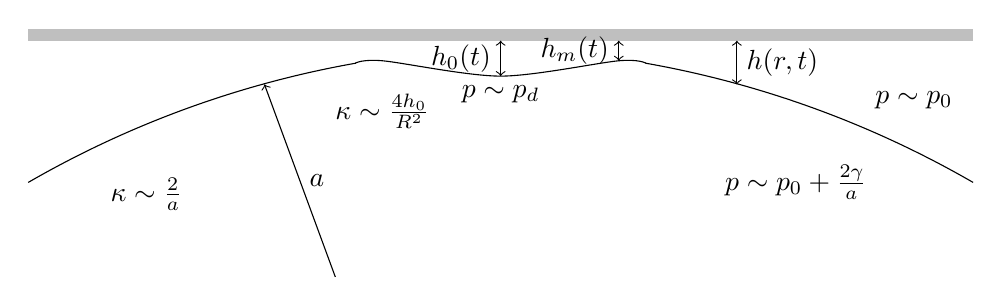
\begin{tikzpicture}[scale=1.5]
		\draw (-4,3) -- (4, 3);
		\fill[gray!50] (-4,3) rectangle (4,3.1);
		\draw (-4,1.8) arc (120:100:8.5);
		\draw (4,1.8) arc (60:80:8.5);
		\draw plot[smooth] coordinates {(-1.23,2.81) (-1, 2.83)
			(0,2.7) (1, 2.83) (1.23, 2.81)};
		\draw[<->] (1, 3) -- (1, 2.83) node[midway,left] {$h_m(t)$};
		\draw[<->] (2, 3) -- (2, 2.63) node[midway, right] {$h(r,t)$};
		\draw (3.5, 2.5) node {$p \sim p_0$};
		\draw (2.5, 1.8) node {$p \sim p_0 + \frac{2\gamma}{a}$};
		\draw[<-] (-2, 2.63) -- (-1.4, 1) node[midway,right] {$a$};
		\draw (-1, 2.4) node {$\kappa \sim \frac{4h_0}{R^2}$};
		\draw[<->] (0,3) -- (0, 2.7) node[midway,left] {$h_0(t)$};
		\draw (-3, 1.7) node {$\kappa \sim \frac{2}{a}$};
		\draw (0, 2.55) node {$p \sim p_d$};
	\end{tikzpicture}
\end{center}

The key idea is the small gap $h_m$ controls a slow leakage flux from the
dimple, which is thus roughly stagnant with uniform pressure
\begin{equation}
	p_d = p_0 + \gamma \left( \frac{2}{a} - \nabla^2 h\right)
\end{equation}

We now sketch the solution. From vertical force balance we have
\begin{equation}
	(p_d - p_0) \pi R \approx \frac{4}{3} \pi a^3 \Delta \rho g
\end{equation}
Hence we find in $r < R$
\begin{align}
	R &\sim a \text{Bo}^{1/2} \\
	\nabla^2 h &\ll \frac{2}{a}
\end{align}

\paragraph{Dimple:} in $r < R$, since $p_d$ is uniform, we have
\begin{equation}
	\nabla^2 h = \frac{1}{r} \frac{\partial}{\partial r} \left( r \frac{\partial
	h}{\partial r}\right) \approx \text{const.}
\end{equation}
Solving for $h$ we find
\begin{equation}
	h \approx h_0 \left( 1- \frac{r^2}{R^2}\right)
\end{equation}
and the trapped volume $V \sim h_0 R^2$.

\paragraph{Small gap:} free surface lubrication theory gives leakage flux 
\begin{equation}
	q = \frac{h^3}{3\mu} (\gamma h_{xx})_x
\end{equation}
where $x = r-R$ is a local coordinate near $h_m$. Clearly $\dot{V} \approx
-2\pi R q $ from which we can deduce an equation for $\dot{h_0}$.

\begin{center}
	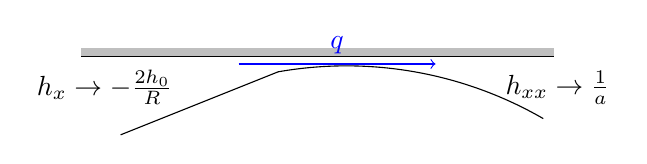
\begin{tikzpicture}
		\draw (-2.5,3) -- (3.5, 3);
		\fill[gray!50] (-2.5,3) rectangle (3.5,3.1);
		\draw (0,2.8) -- (-2, 2);
		\draw (0,2.8) arc (100:60:5); 
		\draw (-2.2, 2.6) node {$h_x \to -\frac{2h_0}{R}$};
		\draw (3.55, 2.6) node {$h_{xx} \to \frac{1}{a}$};
		\draw[blue,->] (-0.5, 2.9) -- (2, 2.9) node[midway,above] {$q$};
	\end{tikzpicture}
\end{center}

We now look for a similarity solution. The scalings are
\begin{equation}
	\frac{h}{x} \sim \frac{h_0}{r}, \hspace{2em} \frac{h^4}{x^3} \sim q \sim
	\frac{h_0}{t}, \hspace{2em} \frac{h}{x^2} \sim 1
\end{equation}
Hence we have $h, h_m \propto t^{-1/2}, \hspace{1em} h_0 \sim t^{-1/4},
\hspace{1em} x \sim t^{-1/4}, \hspace{1em} q \sim t^{-5/4}$, with $\xi =
\frac{x}{Bt^{-1/4}}$, $h = At^{-1/2}H(\xi)$ and suitable constants $A, B$,
chosen so that the unknown flux $\sim 1$ rather than $H'' \to 1$ as $\xi \to
\infty$. From this we deduce an equation for $H$:
\begin{equation}
	H^3 H''' = 1
\end{equation}
with boundary conditions $H' \to -1$ as $\xi \to -\infty$, which is infact 2
conditions that the coefficient of $\xi^2$ goes to 0 and the coefficient of
$\xi$ goes to -1. Hence we find a unique solution to within translation, with
$H_{\text{min}} = 1.2571$ and $H \sim \frac{1}{2}C \xi^2$ as $\xi \to \infty$
with $C = 1.2098$. The unscaled matching condition $h \sim \frac{1}{2a} x^2$
fixes the remaining constants.

\subsubsection{Gravity current on an inclined plane}
Consider a viscous fluid placed on a plane inclined at angle $\theta$ to the
horizontal. We use $x$ as the coordinate parallel and down the plane, $y$
parallel and across the plane, and $z$ perpendicular to the plane. We will
neglect surface tension.
\begin{center}
	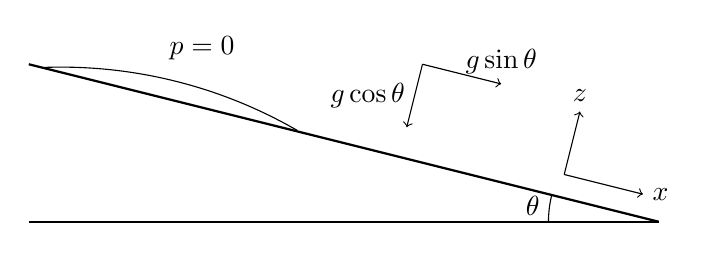
\begin{tikzpicture}[scale=2]
		\draw[thick] (-2, 0) -- (2, 0);
		\draw[thick] (-2, 1) -- (2, 0);
		\draw (1.3,0) arc (180:166:0.7);
		\draw (1.2, 0.1) node {$\theta$};
		\draw (-1.9, 0.98) arc (92:60:3);
		\draw (-0.9, 1.1) node {$p=0$};
		\draw[->] (1.4, 0.3) -- (1.9, 0.175) node [right] {$x$};
		\draw[->] (1.4, 0.3) -- (1.5, 0.7) node[above] {$z$};
		\draw[->] (0.5, 1) -- (1, 1-0.125) node [above] {$g\sin \theta$};
		\draw[->] (0.5, 1) -- (0.4, 0.6) node [midway, left] {$g\cos \theta$};
	\end{tikzpicture}
\end{center}

In our original derivation of the lubrication equations, we neglected body
forces. Hence we must modify the equations to include gravitational force. The
modified $z$-balance is
\begin{align}
	\frac{\partial p}{\partial z} &= -\rho g \cos \theta \\
	\implies p &= \rho g (h(x,y,t) - z)\cos \theta
\end{align}

The modified $x$-balance is similarly
\begin{equation}
	\mu \frac{\partial^2 u}{\partial z^2} = \frac{\partial p}{\partial x} -
	\rho g \sin \theta
\end{equation}

We solve for $\symbf{u}$ to get $\symbf{q}$, then using mass conservation we
find the evolution equation
\begin{equation}
	\frac{\partial h}{\partial t} + \frac{g \sin \theta}{3\nu} \frac{\partial
	h^3}{\partial x} = \frac{g \cos \theta}{3\nu} \nabla \cdot (h^3 \nabla h)
\end{equation}
We can find various similarity solutions to this equation. See Lister, JFM
1992.

\subsubsection{Similarity solutions}
Note we often find similarity solutions of the form $At^\alpha f(\xi \equiv
\frac{x}{Bt^\beta})$. Then
\begin{align}
	\frac{\partial}{\partial x} \left[ At^\alpha f(\frac{x}{Bt^\beta})\right]
	&= \frac{At^\alpha}{Bt^\beta} f'(\xi) \\
	\int \, \diffd x &= Bt^\beta \int \, \diffd \xi \\
	\frac{\partial}{\partial t}\left[ At^\alpha f(\frac{x}{Bt^\beta})\right]
	&= \frac{A t^\alpha}{t} (\alpha f - \beta \xi f'(\xi))
\end{align}
Hence operations work in the same way, but with extra factors, in the same way
the scalings are derived. For this reason, the factors often cancel in the
governing equations.

\begin{eg}
	Thermal diffusion of a heat pulse in 3D.  The  governing equation is
	\begin{equation}
		\frac{\partial T}{\partial t} = \kappa \frac{1}{r^2}
		\frac{\partial}{\partial r} r^2 \frac{\partial T}{\partial r}
	\end{equation}
	with volume constraint
	\begin{equation}
		4\pi \int Tr^2 \, \diffd r = Q
	\end{equation}
	Consider the scalings of these two equations.
	\begin{equation}
		\frac{T}{t} \sim \frac{\kappa T}{r^2}, \hspace{2em} Tr^3 \sim Q
	\end{equation}
	Hence $r \sim \sqrt{\kappa t}, \hspace{1em} T \sim \frac{Q}{(\kappa
	t)^{3/2}}$. Motivated by these scalings, try similarity solution $T =
	\frac{Q}{(\kappa t)^{3/2}} f(\xi \equiv \frac{r}{\sqrt{\kappa t}})$. Then
	\begin{equation}
		-\frac{3}{2}f -\frac{1}{2}\xi f' = \frac{1}{\xi^2}
		\frac{\partial}{\partial \xi} \xi^2 \frac{\partial f}{\partial \xi}
	\end{equation}
	and volume constraint
	\begin{equation}
		4\pi \int_0^\infty f\xi^2 \, \diffd \xi = 1
	\end{equation}
	Hence we find $f = A e^{-\xi^2/4}$ with $A = \frac{1}{(2\pi)^{3/2}}$ by
	the integral constraint.
\end{eg}

\lecture{18/11/20}
\subsubsection{Axisymmetric viscous gravity current}
\label{ss:viscousgravitycurrent}
Consider a fixed volume $V$ of viscous fluid spreading axisymmetrically on a
horizontal plane under air (i.e. a free-surface condition). The equations of
motion and global conservation of mass are
\begin{align}
	\frac{\partial h}{\partial t} &= \frac{g}{3\nu} \frac{1}{r}
	\frac{\partial}{\partial r} \left[ rh^3 \frac{\partial h}{\partial
	r}\right] \\
	V &= 2\pi \int_0^{R(t)} h r \, \diffd r
\end{align}

\begin{center}
	\begin{tikzpicture}[scale=2]
		\draw[thick] (-3,0) -- (3,0);
		\fill[gray!50] (-3,0) rectangle (3,-0.1);
		\draw[dashed] (0,0) -- (0, 1) node[above] {$r=0$};
		\draw (0,0) [partial ellipse = 180:0:2.7 and 0.7];
		\draw (2, 0.65) node {$p=0$};
		\draw (2.7, -0.2) node {$R(t)$};
		\draw[<->] (-2, 0) -- (-2, 0.47) node[midway,right] {$h(r,t)$};
	\end{tikzpicture}
\end{center}

Scaling gives $h/t \sim gh^4 / \nu R^2$ and $hR^2 \sim V$, from which we
deduce
\begin{align}
	h &\sim \left( \frac{\nu V}{gt}\right)^{1/4} \\
	r &\sim \left( \frac{gV^3 t}{\nu} \right)^{1/8}
\end{align}

Hence try similarity solution
\begin{equation}
	h(r,t) = \left( \frac{\nu V}{g t}\right)^{1/4} H(\eta), \hspace{2em} \eta
	\equiv \frac{r}{\left(\frac{gV^3t}{\nu}\right)^{1/8}}
\end{equation}

Substituting into the equation of motion and mass conservation, as expected
the constants cancel and we find
\begin{align}
	2\pi \int_0^\eta H\eta \, \diffd \eta &= 1 \\
	\frac{1}{3\eta}\frac{\diffd}{\diffd \eta} \left[ \eta H^3
	\frac{\diffd H}{\diffd \eta}\right] &= -\frac{1}{4} H - \frac{1}{8} \eta
	H'
\end{align}
subject to $H(\eta_N) = 0$ where the `nose' of the current is at $\eta_N =
R/(gV^3t/\nu)^{1/8}$.  The solution is
\begin{equation}
	H(\eta) = \left( \frac{9}{16}(\eta_N^2 - \eta^2)\right)^{1/3}
\end{equation}
where $\eta_N = (1024/243\pi^3)^{1/8}$.

\subsection{Long Thin Flows II: Extensional flows}
\label{ss:extensional}
We now consider thin flows with effectively stress-free boundaries.
\subsubsection{Axisymmetric case}
\begin{wrapfigure}{R}{0.4\textwidth}
	\begin{tikzpicture}[scale=1.5]
		\draw[smooth,thick,rotate=3] plot[domain=0.2:0.8] ({\x}, {2-1/\x});
		\draw[smooth,thick,rotate=-3] plot[domain=-0.2:-0.8] ({\x}, {2+1/\x});
		\draw (0,0) ellipse (0.5 and 0.1);
		\draw[<->] (2, 1) -- (2, -3) node[midway,right] {$L$};
		\draw (-1.5, 0) node {$A(z) = \pi a^2(z)$};
		\draw[->] (0, -2) -- (0, -2.5) node[below] {$z$};
		\draw[->] (0, -2) -- (0.5, -2) node[right] {$r$};
		\draw[->] (0, 1) -- (0, 0.5) node[below] {$w$};
		\draw[->] (0, 1) -- (0.5, 1) node[right] {$u$};
		\draw[blue,dashed] (-0.43, -0.5) -- (0.43, -0.5);
		\draw[blue,dashed] (-0.4, -1) -- (0.4, -1);
		\draw[blue,->] (-0.25, -0.5) -- (-0.25, -1);
		\draw[blue,->] (0.25, -0.5) -- (0.25, -1);
		\draw[blue,->] (0, -0.5) -- (0, -1);
	\end{tikzpicture}
\end{wrapfigure}

Assume that $\partial_z, \partial_r \sim \frac{1}{L} \ll \frac{1}{a}$.
Assuming no tangential stress, we have $\frac{\partial w}{\partial r} = 0$
hence $w = w(z,t)$ is plug flow. Mass conservation on a slice gives
\begin{align}
	\frac{\partial A}{\partial t} + \frac{\partial}{\partial z} (Aw) &= 0\\
	\implies \frac{\diffD A}{\diffD t} &= -A\frac{\partial w}{\partial z}
\end{align}
i.e. there is thinning of the flow by stretching in the $z$ direction. Local
mass conservation $\nabla \cdot \symbf{u} = 0$ gives
\begin{align}
	\frac{1}{r} \frac{\partial}{\partial r} (ru) + \frac{\partial w}{\partial
	z} &= 0 \\
	\implies u &= -\frac{1}{2} r \frac{\partial w}{\partial z} \label{eq:ext2}
\end{align}
This makes physical sense: there are 3 directions of straining which must sum
to $0$. Horizontally, there is strain in $2$ directions each equal to $u_r$,
and the vertical strain is $w_z$. The radial stress balance is
\begin{align}
	-p + 2\mu \frac{\partial u}{\partial r} &= -p_{\text{ext}} \\
	\implies -p &= -p_{\text{ext}} + \mu \frac{\partial w}{\partial z}
\end{align}

The axial stress is 
\begin{align}
	\sigma_{zz} &= -p + 2\mu \frac{\partial w}{\partial z} \\
			&= -p_{\text{ext}} + 3\mu \frac{\partial w}{\partial z}
\end{align}

Axial force balance on a slice includes the differential stress across the
slice, the external pressure acting normal to the sides, and the axial body
force.
\begin{center}
	\begin{tikzpicture}
		\draw[thick] (-3, 0) -- (3,0) -- (2.5, 2) -- (-2.5, 2) -- (-3,0);
		\draw[->] (0,0) -- (0,-1) node[below] {$A \sigma_{zz}\mid_{z+\delta z}$};
		\draw[->] (0,2) -- (0,3) node[above] {$A\sigma_{zz}\mid_{z}$};
		\draw[<-] (2.75, 1)--(4,1.3)  node[right]{$p_{\text{ext}}\cdot 2\pi a \cdot
		\delta z$};
		\draw[<-](-2.75, 1)--(-4,1.3) node[left] {$p_{\text{ext}}\cdot 2\pi a \cdot
		\delta z$};
		\draw[->] (-1.5, 1) -- (-1.5, -1.5) node[below] {$A\delta z f$};
		\draw[fill=black] (-1.5,1) circle (0.1);
		\draw (3,0) node[right] {$z+\delta z$};
		\draw (2.5, 2) node[right] {$z$};
	\end{tikzpicture}
\end{center}

\begin{equation}
	\frac{\partial}{\partial z}(A\sigma_{zz}) + p_{\text{ext}} \frac{\partial
	A}{\partial z} + A f = 0
\end{equation}
Hence using above results
\begin{equation}
	\frac{3\mu}{A} \frac{\partial}{\partial z} (A\frac{\partial w}{\partial
		z}) - \frac{\partial p_{\text{ext}}}{\partial z} + f =
		0\label{eq:ext1}
\end{equation}

Equations \eqref{eq:ext1} and \eqref{eq:ext2} can be used to solve the problem. 

\paragraph{Variations.}
\begin{enumerate}
	\item Add surface tension: add $\frac{\gamma}{a}$ to $p_{\text{int}}$ and
		add $\gamma\left[ 2\pi a(z+\delta z) - 2\pi a(z)\right]$ to the axial
		force balance. Equivalently (and more simply) add $\frac{\gamma}{a}$
		to $p_{\text{ext}}$ in \eqref{eq:ext1}.
	\item Unidirectional extension of a sheet simply has $u_x = -w_z$ and $A$
		is replaced with $h$, and an extensional viscosity $4\mu$ instead of
		$3\mu$. General extension of a sheet has coupling terms between $u$
		and $w$. For example;
	\item Radial extension of a sheet. \vspace{0.5in}
		
		\begin{center}
			\begin{tikzpicture}
				\draw[thick] (0,0) ellipse (3 and 0.2);
				\draw[thick] (0,-4.37) [partial ellipse=127:53:5 and 5.5];
				\draw[<->] (1, -0.18) -- (1, 0.18) node[midway,right] {$h(r,t)$};
				\draw[->,blue] (0.8, 0.22) -- (1.5, 0.65);
				\draw[->,blue] (-0.8, 0.22) -- (-1.5, 0.65);
				\draw[->,blue] (0,0.24) -- (0, 0.9);
				\draw[thick] (7,0) circle (2);
				\draw[dashed] (7-1.6,1.2) -- (7+1.6, 1.2);
				\draw[->] (5, 1.5) arc (70:120:3);
				\draw (3.75, 2) node {slice};
				\draw[blue,->] (7,0) -- (8.5,0);
				\draw[blue,->] (7,0) -- (5.5,0);
				\draw[blue,->] (7,0) -- (7,1.5);
				\draw[blue,->] (7,0) -- (7,-1.5);
				\draw[blue,->] (7,0) -- (7+1.061,1.061);
				\draw[blue,->] (7,0) -- (7-1.061,1.061);
				\draw[blue,->] (7,0) -- (7+1.061,-1.061);
				\draw[blue,->] (7,0) -- (7-1.061,-1.061);
				\pgfresetboundingbox
			\end{tikzpicture}
		\end{center}
		
		The velocity has only radial and
		vertical components, $\symbf{u} = (u, 0, w)$. \\ We have $u=u(r,t)$ and
		from incompressibility 
		\begin{equation}
			\frac{\partial w}{\partial z} =
			-\frac{1}{r}\frac{\partial}{\partial r} (ru)
		\end{equation}
		Following a similar derivation as before we also find
		\begin{align}
			-p + 2\mu \frac{\partial w}{\partial z} &= -p_{\text{ext}} \\
			e_{rr} &= \frac{\partial u}{\partial r} \\
			e_{\theta\theta} &= \frac{u}{r} \\
			e_{\theta\theta} + e_{rr} + e_{zz} &= 0
		\end{align}
		From these results we can find $\sigma_{rr}$ and
		Consider a force balance on a `pineapple slice' of small angle $\delta
		\theta$ and radial length $\delta r$.
		\begin{center}
			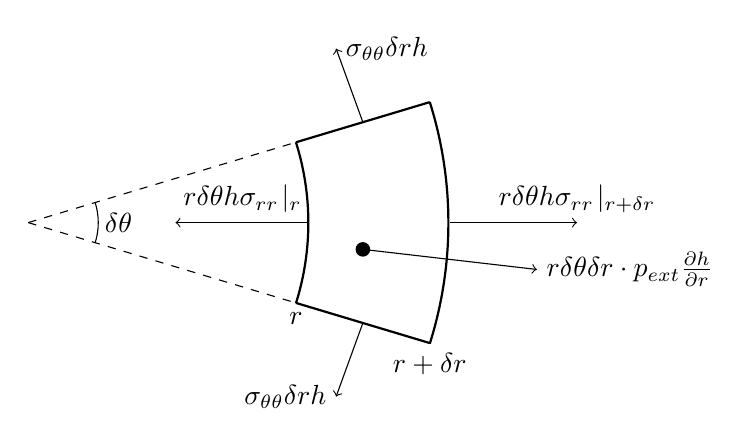
\begin{tikzpicture}[scale=1.7]
				\draw[thick] (3,0.9) arc (17.5:-17.5:3);
				\draw[thick] (2,0.6) arc (17.5:-17.5:2);
				\draw[dashed] (0,0) -- (2,0.6);
				\draw[dashed] (0,0) -- (2,-0.6);
				\draw[thick] (2,0.6) -- (3, 0.9);
				\draw[thick] (2,-0.6) -- (3, -0.9);
				\draw[->] (2.1, 0) -- (1.1, 0) node[midway,above] {$r \delta
				\theta h \sigma_{rr}\!\mid_r$};
				\draw[->] (3.15, 0) -- (4.1, 0) node[above] {$r \delta
				\theta h \sigma_{rr}\!\mid_{r+\delta r}$};
				\draw[->] (2.5, 0.75) -- (2.3, 1.3) node[right]
				{$\sigma_{\theta\theta} \delta r h$};
				\draw[->] (2.5, -0.75) -- (2.3, -1.3)node[left]
				{$\sigma_{\theta\theta} \delta r h$};
				\draw (0.5, 0.15) arc (17.5:-17.5:0.5);
				\draw (0.5, 0) node[right] {$\delta\theta$};
				\draw (2,-0.6) node[below] {$r$};
				\draw (3,-0.9) node[below] {$r+\delta r$};
				\draw[fill] (2.5, -0.2) circle (0.05);
				\draw[->] (2.5, -0.2) -- (3.8, -0.35) node[right] {$r \delta
					\theta \delta r \cdot p_{\text{ext}} \frac{\partial
				h}{\partial r}$};
			\end{tikzpicture}
		\end{center}
		\begin{equation}
			\implies \frac{\partial}{\partial r} (r h \sigma_{rr}) -
			h\sigma_{\theta\theta} + r p_{\text{ext}} \frac{\partial
			h}{\partial r} = 0
		\end{equation}
		For further details, see SVF exam 2019 question 2.
	\item Can include inertia $\rho \frac{\diffD w}{\diffD t}$ on RHS of
		\eqref{eq:ext1} when $\frac{w L}{\nu} \sim 1$.
	\item Adding a lateral force gives a rapid response by bending (low
		resistance compared to stretching).
\end{enumerate}

\lecture{20/11/20}
\subsubsection{Viscous thread falling under gravity}
Consider a thread of viscous fluid injected through a gap with volume flux
$Q$. The cross-sectional area of the thread is $A(z)$ with velocity $\symbf{u}
= w\hat{\symbf{z}}$ only. We will consider both the steady behaviour and the
transient case when the thread has length $L(t)$ and a stress free bottom.
The internal pressure is assumed hydrostatic.

\begin{center}
	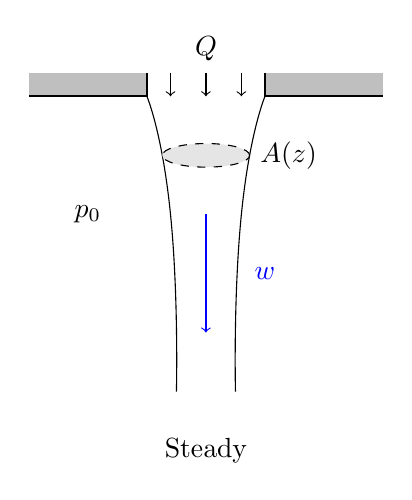
\begin{tikzpicture}[scale=1.5]
		\fill[gray!50] (-1.5,3) rectangle (-0.5,3.2);
		\fill[gray!50] (0.5,3) rectangle (1.5, 3.2);
		\draw[thick] (-1.5, 3) -- (-0.5,3) -- (-0.5,3.2);
		\draw[thick] (0.5,3.2) -- (0.5, 3) -- (1.5, 3);
		\draw[blue,->] (0, 2) -- (0,1);
		\draw[blue] (0.5, 1.5) node {$w$};
		\draw[smooth] plot[tension=1] coordinates {(0.5, 3) (0.3, 2) (0.25,
		0.5)};
		\draw[smooth] plot[tension=1] coordinates {(-0.5, 3) (-0.3, 2) (-0.25,
		0.5)};
		\draw[dashed,fill=gray!20] (0,2.5) ellipse (0.37 and 0.1);
		\draw (0.7, 2.5) node {$A(z)$};
		\draw (-1, 2) node {$p_0$};
		\draw[->] (-0.3, 3.2) -- (-0.3, 3);
		\draw[->] (0.3, 3.2) -- (0.3, 3);
		\draw[->] (0, 3.2) -- (0, 3);
		\draw (0, 3.4) node {$Q$};
		\draw (0, 0) node {Steady};
	\end{tikzpicture}
	\qquad
	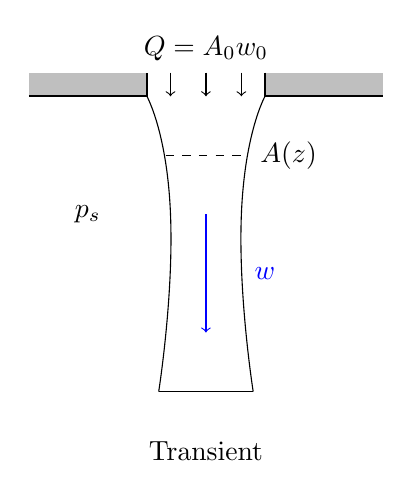
\begin{tikzpicture}[scale=1.5]
		\fill[gray!50] (-1.5,3) rectangle (-0.5,3.2);
		\fill[gray!50] (0.5,3) rectangle (1.5, 3.2);
		\draw[thick] (-1.5, 3) -- (-0.5,3) -- (-0.5,3.2);
		\draw[thick] (0.5,3.2) -- (0.5, 3) -- (1.5, 3);
		\draw[blue,->] (0, 2) -- (0,1);
		\draw[blue] (0.5, 1.5) node {$w$};
		\draw[smooth] plot[tension=1] coordinates {(0.5, 3) (0.3, 2) (0.4,
		0.5)};
		\draw[smooth] plot[tension=1] coordinates {(-0.5, 3) (-0.3, 2) (-0.4,
		0.5)};
		\draw (0.4, 0.5) -- (-0.4, 0.5);
		\draw[dashed] (-0.34, 2.5) -- (0.34, 2.5);
		\draw (0.7, 2.5) node {$A(z)$};
		\draw (-1, 2) node {$p_s$};
		\draw[->] (-0.3, 3.2) -- (-0.3, 3);
		\draw[->] (0.3, 3.2) -- (0.3, 3);
		\draw[->] (0, 3.2) -- (0, 3);
		\draw (0, 3.4) node {$Q = A_0 w_0$};
		\draw (0, 0) node {Transient};
	\end{tikzpicture}
\end{center}

The governing equations in both cases are
\begin{align}
	3\mu \frac{\partial}{\partial z} \left[ A \frac{\partial w}{\partial z}
	\right] &= -\rho g A \\
	\frac{\partial A}{\partial t} + \frac{\partial}{\partial z} \left[ A w
		\right] &= 0 \\
		\text{or}\hspace{1em}
	\frac{\diffD A}{\diffD t} &= -A \frac{\partial w}{\partial z}
\end{align}

\paragraph{Steady case.}
From mass conservation, we have $Aw = Q$. Hence
\begin{equation}
	\frac{w}{Q} \frac{\diffd}{\diffd z} \left[ \frac{Q}{w} \frac{\diffd
	w}{\diffd z} \right] = -\frac{\rho g}{3\mu}
\end{equation}

This can be solved exactly in the general case. The solution with $A
\frac{\diffd w}{\diffd z} \to 0$ as $z \to \infty$ is 
\begin{align}
	w &= \frac{g}{6\nu} (z-z_0)^2 \\
	A &= \frac{6Q \nu}{g} \frac{1}{(z-z_0)^2}
\end{align}
where the constant $z_0$ is an origin chosen so that $A = A_0$ at $z=0$. We
now check the validity of our assumptions.

\begin{itemize}
	\item Slenderness is valid if $\frac{a}{L} \ll 1$. Hence $A^{1/2}/(z-z_0)
		\ll 1$
		\begin{equation}
			\implies z - z_0 \gg \left(\frac{6Q\nu}{g}\right)^{1/4} \sim a_0
		\end{equation}
	\item Inertia is negligible if $\frac{wL}{\nu} \sim
		\frac{g(z-z_0)^3}{6\nu^2} \ll 1$
		\begin{equation}
			\implies z - z_0 \ll \left( \frac{6\nu^2}{g}\right)^{1/3}
		\end{equation}
		For syrup with $\nu \sim 300 \,cm^2 s^{-1}$, this distance is
		approximately $9\,cm$.
\end{itemize}

Note that for large $z$, the dominant balance is
\begin{equation}
	\rho w \frac{\partial w}{\partial z} \sim \rho g \implies w \sim
	\sqrt{2gz}
\end{equation}
hence the parts of the thread far from $z=0$ are in free fall.

\paragraph{Transient evolution.}
Integrating the governing equation for $w$ we have
\begin{equation}
	3 \mu A \frac{\partial w}{\partial z} = \rho g \int_z^{L(t)} A \, \diffd z 
\end{equation}
This says that viscous stress balances the weight of the fluid. Re-arranging
this equation allows use of the governing equation for $A$:
\begin{equation}
	A \frac{\partial w}{\partial z} = \frac{6}{3\nu} \int_z^{L(t)} A \, \diffd
	z = -\frac{\diffD A}{\diffD t}
\end{equation}
Hence a material slice thins due to the weight below it. To proceed we label
material slices by their `release time' $t_0$. Hence we replace
$\frac{\diffD}{\diffD t}$ with $\left.\frac{\diffd}{\diffd t}\right|_{t_0}$
and note $\int_z^L A \, \diffd z = Q t_0$.
\begin{center}
	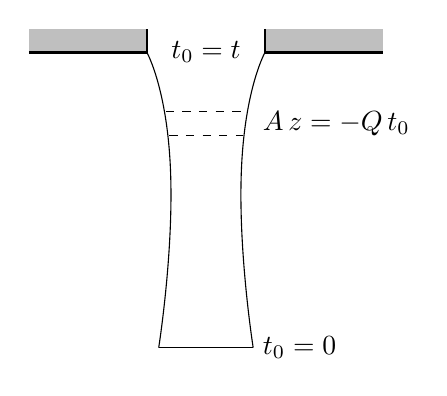
\begin{tikzpicture}[scale=1.5]
		\fill[gray!50] (-1.5,3) rectangle (-0.5,3.2);
		\fill[gray!50] (0.5,3) rectangle (1.5, 3.2);
		\draw[thick] (-1.5, 3) -- (-0.5,3) -- (-0.5,3.2);
		\draw[thick] (0.5,3.2) -- (0.5, 3) -- (1.5, 3);
		\draw[smooth,name path=C] plot[tension=1] coordinates {(0.5, 3) (0.3, 2) (0.4,
		0.5)};
		\draw[smooth,name path=D] plot[tension=1] coordinates {(-0.5, 3) (-0.3, 2) (-0.4,
		0.5)};
		\draw (0.4, 0.5) -- (-0.4, 0.5);
		\draw[dashed,name path=B] (-0.34, 2.5) -- (0.34, 2.5);
		\draw[dashed,name path=A] (-0.31, 2.3) -- (0.31, 2.3);
		\draw (0.4, 2.4) node[right] {$A\,\diffd z = - Q\, \diffd t_0$};
		\draw (0.4,0.5) node[right] {$t_0=0$};
		\draw (0, 3) node {$t_0=t$};
	\end{tikzpicture}
\end{center}

Hence 
\begin{align}
	\frac{\diffd A}{\diffd t} &= -\frac{gQt_0}{3\nu} \\
	\implies A &= A_0 - \frac{gQt_0}{3\nu}(t-t_0)
\end{align}

Hence $A \to 0$ as $t \to t_0 + \frac{3\nu A_0}{gQ t_0}$ which is minimised at
\begin{equation}
	t^* = 2\left( \frac{3\nu A_0}{g Q}\right)^{1/2}
\end{equation}
and $t_0 = t^*/2$. Hence half the mass breaks off and the evolution continues
with a new weight. We know $A(t;t_0)$, and want to find the shape of the flow,
i.e. $A(z,t)$. Now
\begin{align}
	A \, \diffd z &= -Q \, \diffd t_0 \\
	\implies z(t;t_0) &= \int_{t_0}^t \frac{Q \, \diffd t_0'}{A(t;t_0')}
\end{align}

Let $T = t/(\frac{gQ}{3\nu A_0})^{1/2}$ and $Z = z/(\frac{gQ^3}{3\nu
A_0^3})^{1/2}$. Then
\begin{align}
	A &= 1 - T_0 (T-T_0) \\
	Z &= \frac{2}{\sqrt{4-T^2}} \left[
		\text{arctan}\left(\frac{T}{\sqrt{4-T^2}}\right) - \text{arctan}\left(
	\frac{2T_0-T}{\sqrt{4-T^2}}\right)\right]
\end{align}

As $T \to 2$ we get break-up, with the slice $T_0 = 1$ breaking.

\subsection{Long Thin Flows III: Two-fluid case}
When are boundary conditions effectively rigid or stress free?
\subsubsection{Gravity current along interface between two fluids.}
For simplicity, we assume that the two semi-infinite fluids have the same
viscosity $\mu$, and the fluid pool between the two interfaces has viscosity
$\lambda \mu$.

\begin{center}
	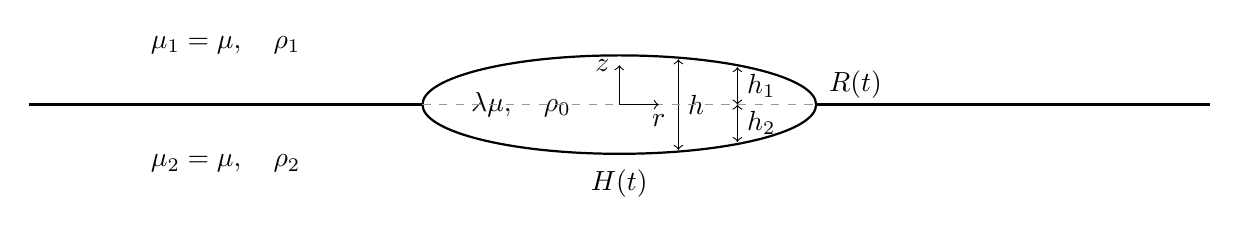
\begin{tikzpicture}[scale=2.5]
		\draw[thick] (-3, 0) -- (-1, 0);
		\draw[thick] (1, 0) -- (3,0);
		\draw[thick] (0,0) ellipse (1 and 0.25);
		\draw (-0.5,0) node {$\lambda \mu, \hspace{1em} \rho_0$};
		\draw (-2, 0.3) node {$\mu_1 = \mu, \hspace{1em} \rho_1$};
		\draw (-2, -0.3) node {$\mu_2 = \mu, \hspace{1em} \rho_2$};
		\draw[<->] (0.3, -0.23) -- (0.3, 0.23) node[midway,right] {$h$};
		\draw[<->] (0.6, -0.19) -- (0.6,0) node[midway,right] {$h_2$};
		\draw[<->] (0.6, 0) -- (0.6, 0.19) node[midway,right] {$h_1$};
		\draw[dashed,thin,gray!80] (-1,0) -- (1,0);
		\draw[->] (0,0) -- (0.2, 0) node[below] {$r$};
		\draw[->] (0,0) -- (0, 0.2) node[left] {$z$};
		\draw (0, -0.4) node {$H(t)$};
		\draw (1.2, 0.1) node {$R(t)$};
	\end{tikzpicture}
\end{center}

\lecture{23/11/20}
At large times, we expect $R \gg H$. Hence the vertical balance is
hydrostatic. We can deduce the form of pressure in two ways, either by
traversing through the upper fluid or the lower fluid. We have
\begin{align}
	p &= p_0 - \rho_1 g h_1 + \rho_0 g (h_1-z) \hspace{1em} \text{upper path}\\
	  &= p_0 + \rho_2 g h_2 - \rho_0 g(h_2 + z) \hspace{1em} \text{lower path} \\
\end{align}
Given these two forms must coincide, we deduce $(\rho_0 - \rho_1) h_1 =
(\rho_2 - \rho_0) h_2$, i.e. the gravity current floats iceberg-like due to
differences in density. We also find from the above
\begin{align}
	\frac{\partial p}{\partial r} &= \Delta \rho g \frac{\partial h}{\partial
	r} \\
	\text{where} \,\,\, \Delta \rho &= \frac{(\rho_2 -
	\rho_0)(\rho_0-\rho_1)}{\rho_2 - \rho_1}
\end{align}
drives the radial spreading. The rate of spreading is determined by the
viscous resistance. Consider the scalings for $\frac{R}{H} \gg 1$:
\begin{align}
	\text{Kinematics} \, \implies \,\,\, U &\sim \frac{R}{t} \\
	\text{Volume conservation}\, \implies \,\,\, R^2 H &\sim a^3
\end{align}
where $a$ is the radius of the sphere when the current is initially
undeformed, or equivalently $a = V^{1/3}$ where $V$ is the volume of the
initial current. The radial dynamics give
\begin{align}
	\text{Total spreading force} \,\,\, \sim \frac{\partial p}{\partial r}
	\times \text{volume} &\sim \Delta \rho g a^3 \frac{H}{R} \\
	\text{Viscous resistance} &\sim \mu_s \frac{U}{L_s} A_s
\end{align}
where $\mu_s$ is the viscosity, $L_s$ is the lengthscale of the dominant
source of viscous stress, and $A_s$ is the area on which it acts. Hence the
radial balance is
\begin{equation}
	\Delta \rho g a^3 \frac{H}{R} \sim \mu_s \frac{R}{tL_s} A_s
\end{equation}
Define a dimensionless time $\tau \equiv \frac{\Delta \rho g a t}{\mu}$.
Then
\begin{align}
	\frac{R^2 A_s}{a^2 HL_s} \frac{\mu_s}{\mu} &\sim \tau \\
	R^2 H &\sim a^3
\end{align}
which is 2 equations for $R(\tau), H(\tau)$ once $A_s, L_s, \mu_s$ determined.
There are four possibilities for $(\mu_s, L_s, A_s)$ depending on $\lambda$
and $R/H$, in which the dominant behaviour is determined by the relative
important of extreme viscosity contrasts and extreme aspect ratio.

\begin{enumerate}
	\item $\lambda \gg R/H$: internal strain dominates. The external fluid
		appears inviscid. The very viscous internal fluid stretches in
		extensional flow (cf. radial version of extensional flow in
		section~\ref{ss:extensional}).  The internal flow behaves like plug
		flow.
		\begin{center}
			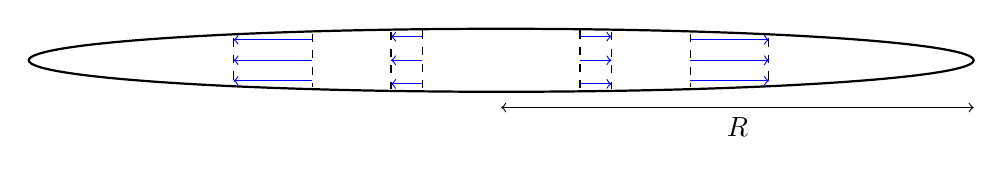
\begin{tikzpicture}[scale=2]
				\draw[thick] (0,0) ellipse (3 and 0.2);
				\draw[<->] (0, -0.3) -- (3, -0.3) node[midway,below] {$R$};
				\draw[dashed] (0.5, 0.19) -- (0.5, -0.19);
				\draw[dashed] (0.7, 0.18) -- (0.7, -0.18);
				\draw[blue,->] (0.5, 0.15) -- (0.7, 0.15);
				\draw[blue,->] (0.5, -0.15) -- (0.7, -0.15);
				\draw[blue,->] (0.5, 0) -- (0.7, 0);
				\draw[dashed] (1.2, 0.17) -- (1.2, -0.17);
				\draw[dashed] (1.7, 0.14) -- (1.7, -0.14);
				\draw[blue,->] (1.2, 0.13) -- (1.7, 0.13);
				\draw[blue,->] (1.2, -0.13) -- (1.7, -0.13);
				\draw[blue,->] (1.2, 0) -- (1.7, 0);
				\draw[dashed] (-0.5, 0.19) -- (-0.5, -0.19);
				\draw[dashed] (-0.7, 0.18) -- (-0.7, -0.18);
				\draw[blue,->] (-0.5, 0.15) -- (-0.7, 0.15);
				\draw[blue,->] (-0.5, -0.15) -- (-0.7, -0.15);
				\draw[blue,->] (-0.5, 0) -- (-0.7, 0);
				\draw[dashed] (-1.2, 0.17) -- (-1.2, -0.17);
				\draw[dashed] (-1.7, 0.14) -- (-1.7, -0.14);
				\draw[blue,->] (-1.2, 0.13) -- (-1.7, 0.13);
				\draw[blue,->] (-1.2, -0.13) -- (-1.7, -0.13);
				\draw[blue,->] (-1.2, 0) -- (-1.7, 0);
			\end{tikzpicture}
		\end{center}
		Hence we have $\mu_s = \lambda \mu$, $L_s \sim R$ and $A_s \sim HR$.
		Then
		\begin{equation}
			\frac{R}{a} \sim \left( \frac{\tau}{\lambda}\right)^{1/2}
		\end{equation}
	\item $\frac{H}{R} \ll \lambda \ll \frac{R}{H}$: external shear dominates.
		Internal fluid is still approximately plug flow, but now resisted by
		shear stress in the external fluid.
		\begin{center}
			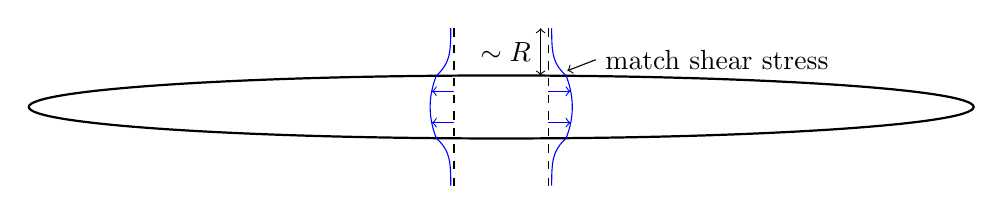
\begin{tikzpicture}[scale=2]
				\draw[thick] (0,0) ellipse (3 and 0.2);
				\draw[dashed] (0.3, 0.5) -- (0.3, -0.5);
				\draw[smooth,blue] plot[domain=-0.1981:0.1981,variable=\y]
				({0.412+0.1981*0.1981 - \y*\y},{\y});
				\draw[smooth,blue] plot[domain=-0.5:-0.1981,variable=\y]
				({0.32+0.3*exp(-30*\y*\y)},{\y});
				\draw[smooth,blue] plot[domain=0.1981:0.5,variable=\y]
				({0.32+0.3*exp(-30*\y*\y)},{\y});
				\draw[blue,->] (0.3, 0.1) -- (0.441, 0.1);
				\draw[blue,->] (0.3, -0.1) -- (0.441, -0.1);
				\draw[dashed] (-0.3, 0.5) -- (-0.3, -0.5);
				\draw[smooth,blue] plot[domain=-0.1981:0.1981,variable=\y]
				({-0.412-0.1981*0.1981 + \y*\y},{\y});
				\draw[smooth,blue] plot[domain=-0.5:-0.1981,variable=\y]
				({-0.32-0.3*exp(-30*\y*\y)},{\y});
				\draw[smooth,blue] plot[domain=0.1981:0.5,variable=\y]
				({-0.32-0.3*exp(-30*\y*\y)},{\y});
				\draw[blue,->] (-0.3, 0.1) -- (-0.441, 0.1);
				\draw[blue,->] (-0.3, -0.1) -- (-0.441, -0.1);
				\draw[<->] (0.25, 0.2) -- (0.25, 0.5) node[midway,left] {$\sim
				R$};
				\draw[<-] (0.42, 0.23) -- (0.6, 0.3) node[right] {match shear stress};
			\end{tikzpicture}
		\end{center}
		The external fluid sees the current as a flat disc of radial
		Stokeslets (cf. integral representations in
		section~\ref{ss:integralrep}). We have $\mu_s \approx \mu, L_s \sim R,
		A_s \sim R^2$ hence
		\begin{equation}
			\frac{R}{a} \sim \tau^{1/5}
		\end{equation}
	\item $\frac{H}{R \ln R/H} \ll \lambda \ll \frac{H}{R}$: internal sehar
		dominates. Poiseuille component of internal flow now much larger than
		the velocity at which external fluid is dragged along (cf. lubrication
		theory in section~\ref{ss:lube}). Effectively no-slip boundaries.
		\begin{center}
			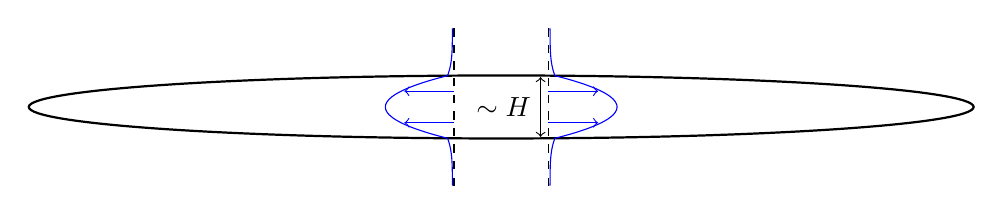
\begin{tikzpicture}[scale=2]
				\draw[thick] (0,0) ellipse (3 and 0.2);
				\draw[dashed] (0.3, 0.5) -- (0.3, -0.5);
				\draw[smooth,blue] plot[domain=-0.1987:0.1987,variable=\y]
				({0.341+10*0.1987*0.1987 - 10*\y*\y},{\y});
				\draw[smooth,blue] plot[domain=-0.5:-0.1987,variable=\y]
				({0.31+0.1*exp(-30*\y*\y)},{\y});
				\draw[smooth,blue] plot[domain=0.1987:0.5,variable=\y]
				({0.31+0.1*exp(-30*\y*\y)},{\y});
				\draw[blue,->] (0.3, 0.1) -- (0.615, 0.1);
				\draw[blue,->] (0.3, -0.1) -- (0.615, -0.1);
				\draw[dashed] (-0.3, 0.5) -- (-0.3, -0.5);
				\draw[smooth,blue] plot[domain=-0.1987:0.1987,variable=\y]
				({-0.341-10*0.1987*0.1987 + 10*\y*\y},{\y});
				\draw[smooth,blue] plot[domain=-0.5:-0.1987,variable=\y]
				({-0.31-0.1*exp(-30*\y*\y)},{\y});
				\draw[smooth,blue] plot[domain=0.1987:0.5,variable=\y]
				({-0.31-0.1*exp(-30*\y*\y)},{\y});
				\draw[blue,->] (-0.3, 0.1) -- (-0.615, 0.1);
				\draw[blue,->] (-0.3, -0.1) -- (-0.615, -0.1);
				\draw[<->] (0.25, -0.19) -- (0.25, 0.19) node[midway,left]
				{$\sim H$};
			\end{tikzpicture}
		\end{center}
		In this case we have $\mu_s \approx \lambda \mu$, $L_s \sim H$, $A_s
		\sim R^2$. Hence
		\begin{equation}
			\frac{R}{a} \sim \left( \frac{\tau}{\lambda}\right)^{1/8}
		\end{equation}
		Note this is the same scaling as the rigid surface case in
		section~\ref{ss:viscousgravitycurrent}, as the balances are the same
		in both problems.
	\item $\lambda \ll \frac{H}{R \ln R/H}$: `push' at nose dominates, i.e.
		bubble regime. Very low viscosity internal fluid moves along the
		current with negligible pressure drop, but must push the external
		fluid out of the way at the nose. The current has a rounded nose and
		away from the nose, $h$ is approximately constant.
		\begin{center}
			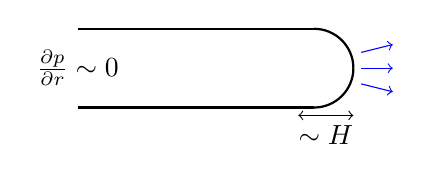
\begin{tikzpicture}
				\draw[thick] (0, 0.5) -- (3, 0.5);
				\draw[thick] (0, -0.5) -- (3, -0.5);
				\draw[thick] (3, 0.5) arc (90:-90:0.5);
				\draw (0,0) node {$\frac{\partial p}{\partial r} \sim 0$};
				\draw[<->] (2.8, -0.6) -- (3.5, -0.6) node[midway,below] {$\sim
				H$};
				\draw[blue,->] (3.6, 0) -- (4, 0);
				\draw[blue,->] (3.6, -0.2) -- (4,-0.3);
				\draw[blue,->] (3.6, 0.2) -- (4,0.3);
			\end{tikzpicture}
		\end{center}
		The external fluid sees an expanding ring force (cf. slender-body
		theory in section~\ref{ss:slenderbody}). We have $\mu_s \approx \mu,
		L_s \sim H \ln R/H, A_s \sim HR$. Hence
		\begin{equation}
			\frac{R}{a \ln R/H} \sim \tau^{1/5}
		\end{equation}
\end{enumerate}

Note that in all four regimes, analytic similarity solutions exist. Also, for
all $\lambda$, the eventual regime as $\tau \to \infty$ is case 2 (Lister \&
Kerr, JFM, 1989).
































\end{document}
